% Belief Updating and Misinformation - Latex file

\documentclass{article}
\usepackage[utf8]{inputenc}

% Layout
\usepackage[a4paper, total={6.5in, 9.5in}]{geometry}
\linespread{1.5}
\usepackage{appendix}
\usepackage[section]{placeins} % ensures figures/tables are in correct section

% References & citation style
\usepackage{natbib}
\bibliographystyle{apalike}
\setcitestyle{authoryear,open={(},close={)}}

% Including graphics
\usepackage{graphicx}
\graphicspath{ {./images/} }

% Creating graphs
\usepackage{tikz}
\usetikzlibrary{arrows,shapes}  

% Math notation
\usepackage{amsmath, amsthm}

% Formatting
\newtheorem{result}{Result}
\newenvironment{Result}{\begin{result} \rm }{\end{result}}

\newcommand*\samethanks[1][\value{footnote}]{\footnotemark[#1]}

% Symbols
\usepackage{eurosym}
\usepackage{xspace} % for space after euro symbol

% For weblink to most recent version
\usepackage{hyperref}


% Title page
\title{Belief Updating with Misinformation}
\author{Lars Wittrock\thanks{\raggedright
    Department of Micro and Public Economics, Maastricht University, The Netherlands. 
    \linebreak \textsc{Contact:} l.wittrock@maastrichtuniversity.nl. 
    \linebreak For helpful comments we thank: Collin Raymond, Yucheng Liang, Joshua Miller, Ted O'Donoghue, Peter Schwardmann, Ori Heffetz, Alex Rees-Jones, Frauke Stehr,
    and seminar audiences at the ESA North America, BERG (Cornell, Wharton and HUJI), Maastricht University.
    }
\and Martin Strobel\samethanks[1]
\and Elias Tsakas\samethanks[1]}

\date{Draft: \today
\\
\href{http://www.larswittrock.eu/UpdatingMisinformation/UpdatingMisinformation.pdf}{Click here for most recent version}}

\begin{document}

\maketitle


\begin{abstract}
Uncertain information is frequently confirmed or retracted after people have initially heard it. A large existing literature has studied how people change their beliefs in response to new information, however, how people react to information about previous information is still unclear. We investigate three closely related questions: 1) How do people update their belief in response to being told a previous signal was (un)informative, 2) What is the effect of verifying the informativeness of a signal ex-ante rather than checking information  ex-post, and 3) Do past information checks affect how people react to new uncertain information in the future? To answer these questions we conduct two (online) experiments using a novel modification of the classical ball and urn framework. It is deliberately abstract to avoid the influence of motivated reasoning or other situation specific circumstances. We find that the majority of subjects react to information about information incorrectly. Importantly, we can predict people's belief after the uncertain information is retracted or confirmed based on their initial response. For retractions, people that over-reacted initially end up with a belief higher than their initial prior and vice versa, people that under-reacted initially end up with a belief lower than before. After multiple consecutive retracted signals this leads to beliefs being more dispersed compared to equivalent information that is ex-ante labeled as uninformative. Confirmations or retractions in the past do not seem to affect how people respond to new uncertain information in our setup.

\bigbreak
\noindent\textsc{Keywords:} Belief Updating, Information Uncertainty, Misinformation, Fact-checking, Retractions, Confirmations.

\noindent\textsc{JEL Classification:} D83, D91, C91
\end{abstract}


\newpage

\section{Introduction}

% INFORMATION ABOUT INFORMATION IS COMMON
In many situations it is unclear at first if information is fully reliable. Such situations can be: reading a yellow press news article, hearing a factual claim from a politician or friend/family member, seeing information leaked by an anonymous source or reading an academic working paper before publication. In all of these situations it can (and frequently does) occur that the initially uncertain information is confirmed or retracted at a later point. News paper articles may be confirmed by further outlets or retracted later.\footnote{One example of retracted news articles is USA Today which had to retract 23 news stories that were based on fabricated information (Source: NY Times 16/06/2022: "USA Today to Remove 23 Articles After Investigation Into Fabricated Sources").} Factual claims of politicians are often checked by a variety of different fact-checking organisations such as FactCheck.org or PolitiFact. Initial rumours leaked by anonymous sources frequently get corrected or confirmed, for example by a company having to admit a data breach.\footnote{One example would be Twitter which had to confirm that a data leak exposed over 5 million accounts earlier this year.} Finally, retractions or confirmations also frequently occur with academic articles, for example on the topic of Covid-19. Since the beginning of 2020 over 270 studies on Covid-19 were retracted\footnote{RetractionWatch.org keeps a precise list of retracted papers on Covid-19.}, while at the same time many more were confirmed by peer-reviews.

% RESPONSES ARE HETEROGENOUS
In practice, despite the increasing effort to resolve information uncertainty and especially to correct false information, many people continue to believe information although it has been proven wrong. For example, on the topic of Covid-19, between 15\% and 20\% of US residents continued endorsing statements that were widely known to have been proven wrong \citep{Meyer2020}. Other examples that are frequently mentioned in the literature are child vaccinations leading to autism which is believed by 29\% of adults, Obama being Muslim or born outside of the USA, deceptive advertising for Listerine mouthwash, and weapons of mass destruction being in Iraq \citep{Lewandowsky2012}. All of these topics have in common that a significant share of the population continues to believe information that was objectively and publicly retracted. On the contrary, in some situations the opposite reaction to retractions of previous information may be observed. Consider the example where a jury observes a witness who fabricated a testimony implicating a defendant as guilty. After learning that the witness statement was untrue the jury may in turn deem it more likely than before that the defendant was in fact innocent. A similar case can be found in the popular short story "The Witness for the Prosecution". It seems that in practice people differ in how they respond to retractions of previous information. This calls for understanding the pattern of how people respond to retractions and to information about information more generally.

% CONTRIBUTION AND RQ 
A variety of factors might contribute to the continued belief in false information. A large literature in psychology suggests that people in general continue to be influenced by retracted information, in the sense that there are spillovers in the direction of the initial signal even after information has been retracted \citep[][and references therein]{Ecker2022}. However, most of these studies are based on settings that allow for a variety of different reasons that may lead to continued belief in retracted information. The causal nature of the narrative, cognitive ability of the participant and distrust in the retraction of past information all play a role. Political scientists have also studied the effectiveness of fact-checking information. Similarly, they find that correcting false information is often ineffective \citep{Nieminen2018}. They suggest motivated reasoning and the initial belief as key factors that influence to what extent people respond to retractions of past information. One could also think of further factors such as inattention to retractions or reasoning about the intentions behind fake news that might influence to what extent people react to retractions. We focus on the question of belief updating from \textit{information about information} in general. We want to identify whether the failure to correctly process information about previous information constitutes a novel form of updating bias. 

% WHY AN ABSTRACT EXPERIMENT
To answer this question, we deliberately choose an abstract experimental framework. This allows us to cleanly identify how people react to information about information while excluding confounds such as motivated reasoning or distrust in retractions. Note that this is a conservative approach, in the sense that any context-dependent factors will likely amplify any effects we may find. For instance, if people continue believing that Obama is Muslim regardless of their political preferences, one would imagine the effect to be even stronger among Republicans. To the best of our knowledge, the only other paper in the literature that studies this problem from this angle is the one by \cite{Goncalves2022}, which we will further discuss later on. 
% PRECISE DESIGN 
More specifically, we introduce a novel experimental design that modifies the well-studied existing framework of balls and urns. In the classical setting one of two urns filled with differently colored balls is randomly selected. Each urn contains a majority of balls with its own color and a minority of balls of the other urn color. A ball drawn from the selected urn is therefore a noisy signal for the urn color. Contrary to the classical setting we create signals that may be informative or entirely uninformative about the selected urn. To do so we mix the informative balls from the randomly selected urn with other balls (of the same colors) that are entirely uninformative. We then draw one of these balls and reveal only the color to the subject. While subjects do not know whether a signal was informative or uninformative initially we can unambiguously verify information afterwards. 

% PRECISE RQs AND IDENTIFICATION
The three main research questions we address are: 1) How do people react to retractions/confirmations of previously uncertain information, 2) What is the effect of verifying information ex-ante (i.e. at the same time as seeing the signal), and 3) Do retractions/confirmations in the past affect how people respond to uncertain information in the future? To answer these questions, we compare reported beliefs within as well as across subjects. We look at sequences of reported beliefs, one before a ball is drawn (viz., the prior), one after the ball is drawn and its color is announced (viz., the initial signal), and one upon having announced whether the ball was informative/uninformative (viz., the confirmed/retracted signal). Moreover, in a separate treatment we simultaneously show subjects the color of the ball and whether it is informative or not (viz., the combined signal). For retractions, we compare 1) the prior with the retracted signal; 2) the retracted signal with the prior of all people who have seen the same history of signals excluding the retracted signal; and 3) the retracted signal with the combined signal. Similarly, for confirmations, we compare 1) the confirmed signal to the Bayesian posterior; and 2) the confirmed signal with the combined signal. Finally, we test for the effect of past confirmations/retractions on future belief updating from uncertain signals.

% RESULTS MAIN
We find that how people react to information about previous information mainly depends on how a person reacted to the initial signal. This is the case both for retractions as well as for confirmations. With retractions of previous information, the majority of people does not respond correctly by disregarding the retracted information. Instead, subjects are systematically biased based on their initial response. Subjects who over-reacted to the uncertain information fail to fully unlearn retracted information, while subjects that under-reacted initially over-react to the retraction thereof. Only subjects that updated in a Bayesian way from the uncertain information responded to a retraction thereof correctly. This pattern is not explained by certain subjects consistently under-/over-reporting after the retraction. It is the initial reaction that clearly predicts in which directions beliefs are biased after the retraction. Moreover, our findings are robust to varying the display of information and anchoring does not explain the result. The clean and neutral framing means that this pattern is the result of a new type of belief updating bias. Again, it seems plausible that motivated reasoning in most real-world settings would amplify the effect. Our findings imply that misinformation can influence people's beliefs in predictable ways and beliefs are more dispersed after continued exposure to false information. Even if misinformation is corrected immediately after it is shown, the vast majority of people end up with biased beliefs. After multiple consecutive retractions, beliefs are substantially more dispersed compared to beliefs after information that is labeled ex-ante as uninformative. In practice this can have substantial implications in a variety of settings, for example beliefs about politics.

% FURTHER RESULTS
We further find that subjects tend to under-react to confirmations of previously uncertain signals. People reacted less to confirmations than expected given their initial update and also reacted less compared to information that is ex-ante labeled as informative. Also, as for retractions, the initial update after the uncertain signal strongly predicts the reaction to the confirmation. Subjects that under-reacted to the initial signal end up with a lower belief after the confirmation than people that initially over-reacted. People that initially reacted in a Bayesian way end up with a belief in the middle of the two. Finally, we analysed whether past confirmations or retractions affect how people respond to new uncertain information in the future. We do not find any effect of past information checks on future updating. It is possible that this is driven by our neutral framework and in practice differences may emerge.

% OUTLINE
In the next section we discuss the related literature. In section 3 we provide a clear framework for uncertain information and the analysis of verifications. Section 4 presents the experimental design which is based on a modification of the commonly used ball and urn framework. In section 5 we present the results on how people respond to retractions and confirmations, ex-ante verifying information and the effect of past information checks on future updating. Finally, section 6 concludes with a discussion of the findings.


\section{Related Literature}

Our paper relates to three separate literatures. Firstly, to the economics literature on belief updating biases. Secondly, to the psychology literature on retractions of information. Thirdly, to the political science literature on fact-checking of misinformation.

\subsubsection*{Economics: Belief updating biases}

Studying biases of information processing was pioneered by \cite{Phillips1966} as well as \cite{Tversky1971, Tversky1974}. Since then a large number of others have studied how people update their beliefs in a variety of settings. \cite{Benjamin2019} provides a comprehensive overview of the literature. He pools the data from all existing studies into a meta analysis and formalizes a clear framework for analysing belief updating. Benjamin finds evidence that in general people under-infer from new information and that people exhibit base-rate neglect, although there is substantial variation across different studies. Moreover, he finds that in situations with sequential information signals people indeed update sequentially rather than pooling all previous information. A number of people have explored further questions related to information processing and choice. \cite{Charness2021} study the choice between differently biased information sources in a laboratory experiment. They find that people make fundamental mistakes in reasoning about the relative informativeness of biased information sources. The majority of people seeks out confirmatory information. \cite{Enke2020} study the formation of beliefs based on memories. To do so they link information to memorable contexts. They find that beliefs are formed based on associative memories from the past. None of these papers mention situations with information uncertainty. \cite{Liang2020} studies a settings with information uncertainty where subjects receive an uncertain signal that is either from a high or low accuracy source. He finds that people under-infer from the uncertain information. A theory of aversion to information uncertainty explains the results. \cite{Epstein2021} and \cite{Shishkin2021} consider a setting with information ambiguity. However, none of these papers considers a setting with additional information about previously uncertain/ambiguous information.

\cite{Goncalves2022} is the paper closest to ours. They study how people respond to retractions of previously uncertain information. They find that subjects perceive retractions of previous information different to informationally equivalent new information. Furthermore, they find that on average subjects fail to fully unlearn retracted information even in a neutral context. This finding is partially contrary to ours. We provide a possible explanation for this result along with our main result. The reason they suggest for biased updating from retractions is that retractions are harder to process than regular new information, therefore leading to mistakes. We propose a different mechanism that is based on the initial response to uncertain information. Moreover, we consider a more general setting of information about previous information. We analyze not only retractions but also confirmations for previous signals.

\subsubsection*{Psychology: Continued Influence Effect}

Psychologists have also studied belief revisions extensively. They mainly consider settings with corrections or refutations of previous information. \cite{Ecker2022} provide a recent review of the literature. We discuss several of these papers below. \cite{Johnson1994} introduced the 'continued influence effect' which states that people continue to be influenced by retracted information. In their setting people continue to rely on retracted information regarding the cause of a warehouse fire. The authors suggest that the reason for this bias is the causal structure of the displayed information. \cite{Roets2017} provide an additional reason: cognitive ability. They study a setting in which participants are asked to evaluate a person on several dimensions based on a variety of information provided to them and one salient piece of information is later retracted. They find that people with high cognitive ability end up with a belief no different to a control group that never saw the retracted information. However, participants with lower cognitive ability continued to rely on the retracted information, leading to the continued influence effect on average. We find some supporting evidence in our setting. People who answered more CRT questions correctly also hold slightly more accurate beliefs after retractions of past information.\footnote{We do not claim that CRT questions are a good measure of cognitive ability, however, they are frequently used in this way \citep[see e.g.][]{Hoppe2011} and likely positively correlated.} Nonetheless, categorizing subjects into types is far less predictive than people's initial response. \cite{Pennycook2021} provide an overview of the psychology of fake news. They discuss extensively why people believe and share fake information. Also they name the lack of careful reasoning as a key driver for the belief in fake information. \cite{Ecker2010} study the influence of ex-ante warning subjects about misinformation. They consider a setting with a causal narrative and retract a key piece of information at a later point. They find that warnings about misinformation reduce the continued influence effect but fail to fully eliminate it. In our setting we provide subjects clear instructions about the informativeness of the information they see. This could also be understood as a warning about misinformation. Finally, \cite{Orear2020} consider a further reason for the continued influence effect. They use the setting from \cite{Ecker2010} and additionally ask participants if they believe the retraction of information. They find that most people do not believe this retraction. They further suggest that some of the wider evidence for the continued influence effect may be due to people not accepting the retraction.

One of the questions we study is closely related to the continued influence effect, however, our experimental design differs to those used in the psychology literature in several ways. We aim to remove any doubt about the credibility of the retraction as well as context dependencies such as different causal structures. We also focus on the statistical inference from retractions rather than memory and recall of past retracted information.


\subsubsection*{Political science: Fact-checking of Misinformation}

The topic of belief in misinformation is also studied in the political science literature. As in the psychology literature, the main focus lies on the correction of false information. \cite{Nieminen2018} provide an overview of the literature on fact-checking of misinformation. While it has become much more popular to check factual information in the last years, results regarding the effectiveness of correcting information are mixed. Some studies find that fact-checking reduces misperceptions while others find that fact-checking is often ineffective. \cite{Walter2020} pool the data from 30 existing studies on fact-checking to evaluate what methods are more or less effective at correcting people's beliefs. They find that in general people do respond to the correction of information by adjusting their beliefs. However, the ability to correct political misinformation depends to a large extent on people's prior belief. Moreover, trust in fact-checking organisations seems to be a further important factor for correcting beliefs. \cite{Thorson2015} studies the persistent effects of corrected misinformation. She finds that even when a correction of previous information is fully believed, misinformation continues to affect attitudes of people. This is the case even when the correction takes place right after people observe misinformation. Also \cite{Uscinski2020} study the question of why people continue to believe disproven information. They focus on Covid-19 theories and find that denialism and conspiracy thinking are among the main drivers. Finally, \cite{Clayton2020} study a method to potentially reduce the influence of misinformation: ex-ante labelling misinformation as false. In the social media environment this method does reduce the influence of misinformation, however, only by a small extent. 

Much of the political science literature focuses on political settings with motivated reasoning. The credibility of a retraction seems to play a large role in how people respond to a retraction. We choose a more neutral framework to remove doubts about the credibility of retractions and to exclude motivated reasoning as a mechanism for biased beliefs. In addition our framework allows us to study confirmations in the same way as retractions.


\section{Framework}

\subsection{Different Types of Signals}

There is a (binary) state space $\Theta=\{\text{Blue }(B), \text{ Red }(R)\}$ together with a full-support prior $p$. There are two stochastic signals -- an informative and a uninformative -- both yielding data from the set $S=\{\text{blue }(b), \text{ red }(r)\}$. 

\begin{itemize}

    \item The \textsc{informative signal} $\pi_I$ reveals the true state with probability $1-\varepsilon>1/2$, i.e., 
    $$\pi_I(b|B)=\pi_I(r|R)=1-\varepsilon.$$ 
    Obviously the larger the parameter $1-\varepsilon$, the more informative $\pi_I$ is. For our experiment we set $\varepsilon=0.25$.
    
    \item The \textsc{uninformative signal} $\pi_U$ provides no information about true state, i.e., for some $\beta\in[0,1]$,
    $$\pi_U(b|B)=\pi_U(b|R)=\beta.$$ 
    This means that no matter which color is drawn from this signal, no updating should take place. The parameter $\beta$ is the probability of drawing blue conditional on the signal being uninformative. For our experiment we take $\beta=0.5$, i.e. uninformative signals are unbiased.

\end{itemize}

In most cases, a subject observes a realized signal without knowing whether it is informative or uninformative. Instead, he assigns probability $\alpha$ it is informative. In our experiment we fix $\alpha=0.4$. So, while $\beta$ is the conditional probability of drawing blue conditional on the signal being uninformative, $1-\alpha$ is the total probability of the signal being uninformative in the first place. 

\begin{itemize}

    \item The \textsc{uncertain signal} aggregates the informative and uninformative signal based on their assigned probabilities, $\alpha$,
    \begin{eqnarray*}
    \pi(b|\theta)&=&\alpha\pi_I(b|\theta)+(1-\alpha)\beta, \\
    \pi(r|\theta)&=&\alpha\pi_I(r|\theta)+(1-\alpha)(1-\beta). 
    \end{eqnarray*}
    Given the parameters used in our experimental setting this implies $\pi(r|R) = \pi(b|B) = 0.6$.
    
\end{itemize}

In some cases, a subject receives information about the previous signal realization. There are two types of signals about previous information.

\begin{itemize}
    
    \item The \textsc{retraction signal} reveals to the subject that the previous uncertain signal was in fact uninformative, i.e. it was generated by $\pi_U$.

    \item The \textsc{confirmation signal} reveals to the subject that the previous uncertain signal was in fact informative, i.e. it was generated by $\pi_I$.

\end{itemize}

Figure \ref{fig:terminology} provides an overview of the different types of information signals a subject may observe. 

\begin{figure}[!ht]
\centering
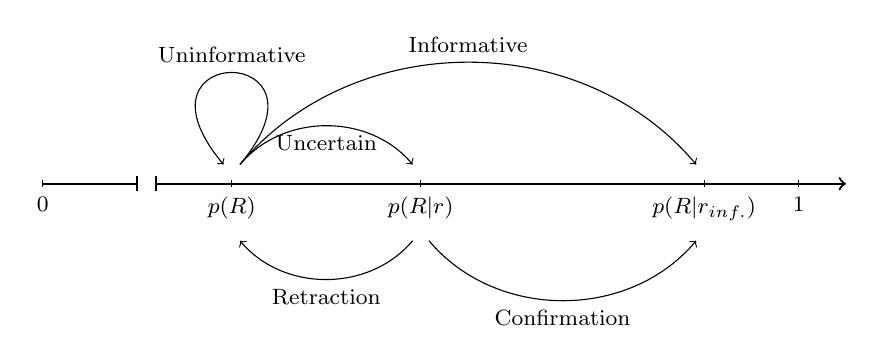
\begin{tikzpicture}[scale=1.2]

% Main axis
\draw[-] [thick] (0,0) -- (1,0);
\draw[->] [thick] (1.2,0) -- (8.5,0);
\draw[][thick] (1,0.08) -- (1,-0.08);
\draw[][thick] (1.2,0.08) -- (1.2,-0.08);
\draw[][] (0,0.04) -- (0,-0.04) node[below] {\footnotesize{0}};
\draw[][] (8,0.04) -- (8,-0.04) node[below] {\footnotesize{1}};

% Beliefs
\draw[][] (2,0.04) -- (2,-0.04) node[below] {\footnotesize{$p(R)$}};
\draw[][] (4,0.04) -- (4,-0.04) node[below] {\footnotesize{$p(R|r)$}};
\draw[][] (7,0.04) -- (7,-0.04) node[below] {\footnotesize{$p(R|r_{inf.})$}};

% Reported beliefs
\node (a) at (2,0.1) {};
\node (b) at (4,0.1) {};
\node (c) at (7,0.1) {};

\draw[->,black] (a) to [out=50,in=130] node[below]{\footnotesize{Uncertain}} (b);
\draw[->,black] (a) to [out=50,in=130] node[above]{\footnotesize{Informative}} (c);
\draw[<-,black] (a) to [out=130,in=50,looseness=25] node[above]{\footnotesize{Uninformative}} (a);

% Rational after retraction
\node (d) at (2,-0.5) {};
\node (e) at (4,-0.5) {};
\node (f) at (7,-0.5) {};

\draw[->] (e) to [out=230,in=310] node[below]{\footnotesize{Retraction}} (d);
\draw[->] (e) to [out=310,in=230] node[below]{\footnotesize{Confirmation}} (f);

\end{tikzpicture}
\caption{\small{Overview of the terminology for the different types of information signals.}}
\label{fig:terminology}
\end{figure}


\subsection{Regular Updating}

In most cases, a subject observes an uncertain signal realisation, without knowing if it is informative or uninformative. If the subject correctly understands the associated probabilities $\alpha$ and $\beta$, and hence correctly puts together the two types of signals, then this type of updating problem is equivalent to most other belief updating settings studied in the literature. Regular updating problems allow for the computation of an objective probability using Bayes' rule. This permits for a clear comparison of reported beliefs to a rational benchmark. Suppose a subject observes a signal realisation $\mathbf{s}$, then the Bayesian posterior belief is given by:
\begin{equation}
\label{eq-bayes}
p(R|\mathbf{s})=\frac{p(R)\pi(\mathbf{s}|R)}{p(B)\pi(\mathbf{s}|B)+p(R)\pi(\mathbf{s}|R)}    
\end{equation}
The initial prior belief, $p_1(R)=p_1(B)=0.5$, is given to the subject. For later rounds ($t>1$) the previously reported belief is assumed to be the prior in the next round, i.e. $p_t(R)=b_{t-1}(R)$ where $b_t(R)$ is the reported belief in round $t$. \cite{Benjamin2019}  finds support for such sequential updating as opposed to subjects aggregating all previous information.

Information processing can be decomposed into the use of prior information and the use of new signals. These two factors are also termed base-rate use and inference. \cite{Grether1980} introduced a reduced-form model to study belief-updating biases. This model is also used by \cite{Benjamin2019}:
\begin{equation}
\label{eq-benjamin}
b(R|\mathbf{s})=\frac{\pi(\mathbf{s}|R)^c p(R)^d}{\pi(\mathbf{s}|R)^c p(R)^d + \pi(\mathbf{s}|B)^c p(B)^d}    
\end{equation}
where $b(\cdot)$ refers to a reported belief, and $c,d\geq 0$. The parameter $c$ measures biased use of the likelihoods (i.e. inference) and the parameter $d$ measures biased use of the priors (i.e. base-rate use). Bayes' Theorem is the special case of $c=d=1$.

\subsection{Updating after Information Checks}

Information checks are signals that clarify previously uncertain signal realisations. In our setting, subjects may learn that a previously uncertain signal was in fact an informative or a uninformative signal. Analysing belief updating from information checks requires a rational benchmark for comparison. As information checks are uninformative without knowledge about the previous signal they are different to observing a regular signal realisation. Below we define the rational Bayesian benchmark for this type of information about information.

\subsubsection*{Retractions}
A retraction informs subjects that the previous signal realisation was uninformative, i.e. it was generated by $\pi_U$. In this case, a rational subject would discard the previous signal and simply return to the belief he had before. Formally, suppose at time $t$ the subject sees a retraction. This implies he saw an uncertain regular signal, $\pi$, in the previous round, $t-1$. He updated his belief from a prior $p_{t-1}(R)$, to a reported posterior, $b_{t-1}(R|\mathbf{s_{t-1}})$. Then in round $t$ that previous signal is retracted. A rational subject should 'forget' the uncertain signal and update his belief as if he never saw that signal. Formally, he should update his belief back to the original prior $p_{t-1}(R)$. The previous belief, $b_{t-1}(R|\mathbf{s_{t-1}})$, should not affect the subject's belief after the retraction of that signal. Importantly, any mistakes a person may make in the initial inference do not matter for the definition of the rational posterior after a retraction. Figure \ref{fig:example_retraction} depicts the rational update for two potential initial reaction to an uncertain signal $r$.

\begin{figure}[h!]
\centering
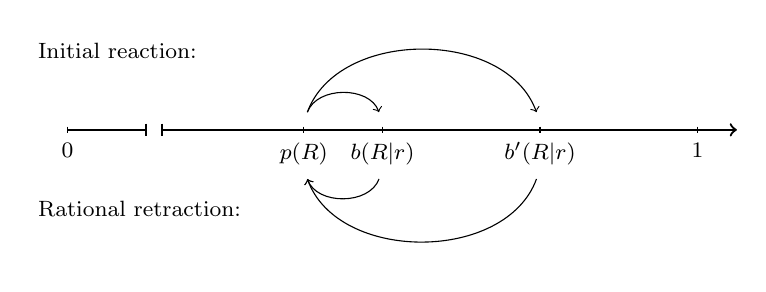
\begin{tikzpicture}[scale=1]

% Main axis
\draw[-] [thick] (0,0) -- (1,0);
\draw[->] [thick] (1.2,0) -- (8.5,0);
\draw[][thick] (1,0.08) -- (1,-0.08);
\draw[][thick] (1.2,0.08) -- (1.2,-0.08);
\draw[][] (0,0.04) -- (0,-0.04) node[below] {\footnotesize{0}};
\draw[][] (8,0.04) -- (8,-0.04) node[below] {\footnotesize{1}};

% Beliefs
\draw[][] (3,0.04) -- (3,-0.04) node[below] {\footnotesize{$p(R)$}};
\draw[][] (4,0.04) -- (4,-0.04) node[below] {\footnotesize{$b(R|r)$}};
\draw[][] (6,0.04) -- (6,-0.04) node[below] {\footnotesize{$b'(R|r)$}};

% Reported beliefs
\node (a) at (3,0.1) {};
\node (b) at (4,0.1) {};
\node (c) at (6,0.1) {};

\draw[][black] (-0.5,1) node[right] {\footnotesize{Initial reaction:}};
\draw[->,black] (a) to [out=70,in=110] node[above]{} (b);
\draw[->,black] (a) to [out=70,in=110] node[above]{} (c);

% Rational after retraction
\node (d) at (3,-0.5) {};
\node (e) at (4,-0.5) {};
\node (f) at (6,-0.5) {};

\draw[][] (-0.5,-1) node[right] {\footnotesize{Rational retraction:}};
\draw[->] (e) to [out=250,in=290] node[above]{} (d);
\draw[->] (f) to [out=250,in=290] node[above]{} (d);

\end{tikzpicture}
\caption{\small{Example belief update. For any initial reaction, the rational response to a retraction is to return to the initial prior.}}
\label{fig:example_retraction}
\end{figure}


\subsubsection*{Confirmations}

A confirmation, denoted by $c$, is a type of signal revealing that the previously uncertain signal realization was in fact generated by $\pi_I$. As before, a rational subject should disregard his previous belief report and update knowing that the signal is in fact informative, using his initial prior $p_{t-1}$. Formally, the rational belief in round $t$, after observing signals $s_{t-1}$ and $c_t$ is given by:
\begin{equation}
\label{eq-confirmation}
p_t(R|\mathbf{s_{t-1},\mathbf{c_t}})=\frac{p_{t-1}(R)\pi_I(\mathbf{s_{t-1}}|R)}{p_{t-1}(B)\pi_I(\mathbf{s_{t-1}}|B)+p_{t-1}(R)\pi_I(\mathbf{s_{t-1}}|R)}    
\end{equation}

When analysing people's reaction to a confirmation signal the posterior as defined above presents some problems. It could be that a person incorrectly updated from the initial regular signal, such that $b_{t-1}(\cdot|\mathbf{s_{t-1}}) \neq p_{t-1}(\cdot|\mathbf{s_{t-1}})$. In this case analysing people's reaction to the confirmation of the previous signal requires an assumption about the cause of the initial mistake. It might be that a person incorrectly put together the two signals $\pi_I$ and $\pi_U$ or that a person incorrectly perceived the informativeness of signal $\pi_I$. The mistake would thus be caused by an incorrect perception of $\alpha$ or $\epsilon$.\footnote{Of course a person could also make both kinds of mistakes. However, this becomes impossible to disentangle.} The Bayesian posterior as defined in equation \ref{eq-confirmation} implicitly assumes that an incorrect belief update after the initial signal, $b_{t-1}(\cdot|\mathbf{s_{t-1}}) \neq p_{t-1}(\cdot|\mathbf{s_{t-1}})$, is purely a result of incorrect understanding of the probability with which a signal is informative, $\alpha$. In other words, had the subject known the signal realisation came from $\pi_I$ he would have updated correctly. 

To allow for the case where people fail to correctly understand the informativeness of $\pi_I$, it is useful to define a separate subjective Bayesian posterior. We can use the initially reported belief, $b_{t-1}(\cdot|\mathbf{s_{t-1}})$, to calculate the 'rational' posterior belief the person may have updated to if he had known the realized ball came from the informative signal, $\pi_I$. Formally, this requires calculating some 'perceived' $\varepsilon'$ based on reformulating Bayes' rule:
\begin{equation*}
    1-\varepsilon' = \frac{p_{t-1}(R)\cdot(4b_{t-1}(R)+3)-7b_{t-1}(R)}{8p_{t-1(R)}\cdot b_{t-1}(R)-4p_{t-1}(R)-4b_{t-1}(R)}
\end{equation*}
The alternative rational posterior, $p'_t(R|\mathbf{s_{t-1},\mathbf{c_t}})$, is then given by:
\begin{equation}
    \label{eq-confirmation-alt}
    p'_t(R|\mathbf{s_{t-1},\mathbf{c_t}})=\frac{p_{t-1}(R)\cdot(1-\varepsilon')}{p_{t-1}(R)\cdot(1-\varepsilon')+p_{t-1}(B)\cdot\varepsilon'}
\end{equation}

Consider the following example, as illustrated in Figure \ref{fig:example_confirmation}. A person has an initial prior belief of 50\%, $p(R)=0.5$. Upon seeing a red ball he updates his belief to $b(R|r)=0.65$. A Bayesian would have updated to $p(R|r)=0.6$. In the next round the person learns that the signal he previously saw was indeed informative. A fully rational Bayesian should forget about his previously reported belief and update given the combination of the two signals. The rational posterior in this case is given by $p(R|r,c)=0.75$. Similarly, a person who updated incorrectly initially because he failed to put the two signals together correctly should rationally arrive at the same posterior belief $p(R|r,c)=0.75$. However, a person who updated incorrectly initially because of a misperception of $1-\varepsilon$, would update to $p'(R|r,c)=0.875$ if he maintains the same bias about $1-\varepsilon$.

\begin{figure}[!htb]
\centering
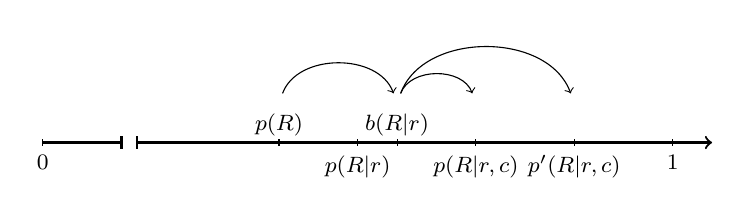
\begin{tikzpicture}[scale=1, align=center]

% Main axis
\draw[-] [thick] (0,0) -- (1,0);
\draw[->] [thick] (1.2,0) -- (8.5,0);

\draw[][thick] (1,0.08) -- (1,-0.08);
\draw[][thick] (1.2,0.08) -- (1.2,-0.08);

\draw[][] (0,0.04) -- (0,-0.04) node[below] {\footnotesize{0}};
\draw[][] (8,0.04) -- (8,-0.04) node[below] 
{\footnotesize{1}};

% Beliefs
\draw[][] (3,0.04) -- (3,-0.04) node[above] {\footnotesize{$p(R)$}};
\draw[][] (4,0.04) -- (4,-0.04) node[below] {\footnotesize{$p(R|r)$}};
\draw[][] (5.5,0.04) -- (5.5,-0.04) node[below] {\footnotesize{$p(R|r,c)$}};

\draw[][] (4.5,0.04) -- (4.5,-0.04) node[above] {\footnotesize{$b(R|r)$}};
\draw[][] (6.75,0.04) -- (6.75,-0.04) node[below] {\footnotesize{$p'(R|r,c)$}};

% Arrows
\node (a) at (3,0.5) {};
\node (b) at (4.5,0.5) {};
\node (c) at (5.5,0.5) {};
\node (d) at (6.75,0.5) {};
\draw[->](a) to [out=70,in=110] node[above]{} (b);
\draw[->](b) to [out=70,in=110] node[above]{} (c);
\draw[->](b) to [out=70,in=110] node[above]{} (d);

\end{tikzpicture}
\caption{\small{Example belief update. Two options could serve as the rational benchmark for analyzing the belief update from the confirmation of a previously uncertain signal.}}
\label{fig:example_confirmation}
\end{figure}


\subsection{Research Questions}
Our framework allows us to test several different research questions. 

\textbf{Question 1.} How do people react to retractions of previous information? We investigate whether subjects initial update after the uncertain information signal, $b_{t-1}$, affects the belief people have following a retraction of that signal. \cite{Goncalves2022} and other papers in the psychology literature find that on average people are biased in the direction of the reported belief. In other words, on average people fail to 'unlearn' retracted information and continue to be influenced by it. We test for a general bias in this form as well as further effects of the initial belief update on beliefs after the retraction.

\textbf{Question 2.} How do people react to confirmations of previous information? Similar to the previous question it seems plausible that the initial belief update shapes how people react to a confirmation of the previous uncertain signal. No previous studies have explicitly tested the impact of signal confirmations on beliefs. Again, we test if people are biased in general when seeing a confirmation as well as what influence the initial update has on beliefs after the confirmation.

\textbf{Question 3.} What is the effect of verifying information ex-ante, i.e. people see the signal and its informativeness at the same time? We hypothesize that more people hold accurate beliefs when information is verified ex-ante. Moreover, we test if beliefs are more dispersed when information is only verified ex-post. 

\textbf{Question 4.} Do information checks in the past affect how people react to uncertain information in the future? Past verifications may influence belief updating in several ways. It could be that people who have seen many retractions/confirmations in the past are more/less critical of new information signals. Moreover, the color of a ball that was retracted/confirmed in the past may influence how people respond to new information. We test if belief updating is influenced in this way by past retractions or confirmations.


\section{Experimental Design}

\subsection{Baseline}
We introduce a novel experimental design that adds information uncertainty to the well-studied ball and urn framework. The design is deliberately abstract because it avoids any context dependencies such as motivated reasoning. Further it removes any doubts about the credibility of a retraction or confirmation of previous information. This unambiguous setting allows for a precise analyse of belief updates. And finally, the similarity with the well-studied ball and urn framework allows for clear comparisons to the existing literature. \cite{Goncalves2022} study a similar modification of the ball and urn framework. Contrary to our setting, their design does not allow for confirmations of previous information.

In the beginning of the experiment there are two urns: a Red urn containing three red balls and one blue ball; and a Blue urn contains three blue balls and one red ball. One of the two urns (Red or Blue) is randomly drawn with equal probability. The subject's task is to estimate the probability that the randomly drawn urn is Red/Blue after receiving hints in the form of ball draws. We modified this standard framework to allow for misinformation. The four balls from the chosen urn are placed inside a black box together with six other, uninformative balls. This means that only four of ten balls are informative hints for the selected urn, i.e. $\alpha=0.4$. Of the six uninformative balls three are red and three are blue, such that uninformative signals are unbiased, i.e. $\beta=0.5$. The subject is shown only the color of one randomly drawn ball from the black box. This ball may be one of the four relevant balls from the urn or one of the six irrelevant balls. An information check tells the subject from which group of balls the previously shown ball came. Figure \ref{fig:instructions} provides a depiction of our experimental design which was also shown to the participants of the study.

\begin{figure}[!htb]
    \centering
    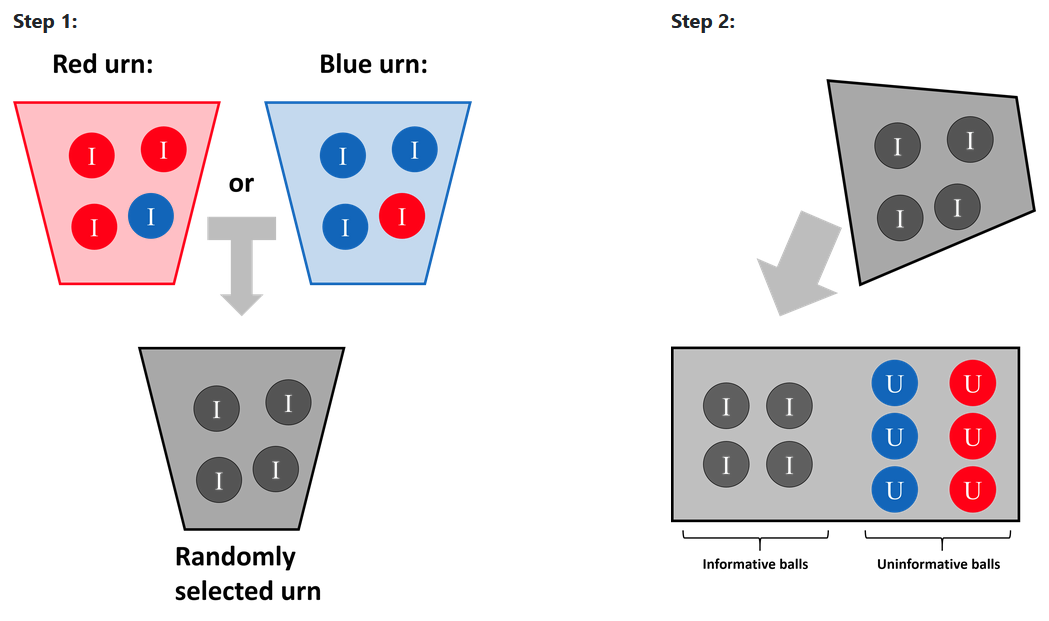
\includegraphics[width = 12cm]{Fig/instructions.png}
    \caption{Experimental design with informative balls and uninformative balls}
    \label{fig:instructions}
\end{figure}

Each subject receives 9 hints about the selected urn in the form of new ball draws (with replacement) and in three rounds it is revealed if the previous ball was in fact informative or not. After each of these 12 information updates subjects report their beliefs about which urn was selected. We systematically vary the rounds in which previous information is checked, however, information checks always take place for three consecutive ball draws. This is done to study the effect of past confirmations/retractions on future updating.


\subsection{Treatment with combined signal}

To answer our third research question, what is the effect of verifying information ex-ante, we run an additional experiment. This experiment is based on the same design as explained above but varies one crucial detail. Instead of ex-post confirming or retracting the previous signal, subjects are immediately shown if a ball is informative or uninformative. Everything else, remains the same. Subjects thus see 6 uncertain signals and 3 signals which are immediately verified as informative or uninformative.


\subsection{Treatments to vary information display}

In the baseline design subjects can see the entire history of signals they have received and the belief they reported last. To make sure the way information is displayed does not influence the results we include additional treatments in all experiments where we either do not display the history of signals or we do not display the previous belief. This allows us to test for effects of anchoring based on presented information as well as potential backward belief revisions.


\subsection{Further design details}

The experiment was programmed using oTree (\cite{Chen2016}) and subjects were recruited from Prolific. We pre-registered outlier criteria and analysis.\footnote{The analysis was slightly modified compared to the pre-registration as we discovered potential problems with the initial framework. We focus on absolute belief differences rather than inference estimated using log-likelihood ratios.} The exact instructions can be found in Appendix \ref{sec:instructions}. All belief reports were incentivized using a quadratic scoring rule. Following \cite{Danz2020}% additional source Che (Christina) Sun, work in progress paper
, we hide the quantitative details of the scoring rules behind an additional button and restrict the main text to a qualitative explanation of the mechanism with an emphasis on its incentive compatibility. Subjects received a completion fee of 2.50\euro\xspace as well as a bonus payment up to 3.00\euro\xspace from the scoring rule mechanism. To enter the main part of the experiment subjects had to answer 5 out of 6 instruction comprehension test questions correctly. In the end of the experiment we attached a post-experiment survey with questions about their strategy and regular demographic questions. 


\section{Results}

The first experiment was conducted in January of 2022 and the second in January 2023. In total 849 subjects completed the experiments from which 96 were removed based on pre-defined criteria.\footnote{These are mainly about subjects not reacting to any of the information on screen, completing the survey faster than possible with reading the instructions or giving primarily dominated responses, i.e. they updated their belief in the wrong direction in the majority of cases.} The median time to complete the experiment was 17 minutes and subjects received on average 4.80\euro. All subjects reported 12 (in experiment 1) or 9 (in experiment 2) beliefs sequentially, leading to a total of 8397 observations used in our analysis. 

\subsection{Preliminaries}

Before analyzing the main research questions regarding information about information we focus on the 'standard' belief updating problems that were also part of our experiment. This serves as a test for the validity of our experimental setting. We modified the standard ball and urn setting which is frequently used in the literature by introducing uncertainty about the informativeness of signals. Besides this our design is similar to most other belief updating experiments and thus allows for a comparison of general results.

Overall, reported beliefs have a high (and significant) correlation with Bayesian posteriors, as reported in Table \ref{tab:belief_bayesian}. Subjects reacted to red and blue signals in a symmetric way implying that the color of the ball had no influence on subjects' behavior. This suggests that in general subjects understood the setup well.\footnote{Some subjects sometimes reported beliefs in the opposite direction from the Bayesian belief. In total about 12.5\% of the observations are such irrational belief reports. Even without any initial filtering (13.6\%) this number is much lower than what was found by \cite{Goncalves2021} in a similar setup (19.5\%).} In the absence of information checks, inference and base-rate use can be estimated, following the methodology introduced in equation \ref{eq-benjamin}. To determine the parameters $c$ and $d$, we estimate the following regression:
\begin{equation}
\label{eq-reg-inference}
ln(\frac{b_t(R|\mathbf{s_t})}{b_t(B|\mathbf{s_t})}) = \alpha + \beta_1 \cdot ln(\frac{p(\mathbf{s_t}|R)}{p(\mathbf{s_t}|B)}) + \beta_2 \cdot ln(\frac{p_t(R)}{p_t(B)}) + \epsilon_t
\end{equation}
where $p_t(R)$ is the prior belief for state $R$ and $p_t(R|\mathbf{s_t})$ is the Bayesian posterior probability for state $R$ associated with signal $s_t$. $\beta_1$ indicates inference from new information ($c$) and $\beta_2$ shows to what extent people rely on their prior, i.e. base-rate use ($d$). 

\begin{Result}
Subjects exhibit significant over-inference ($\beta_1>1$) and base rate neglect ($\beta_2<1$).
\end{Result}

The detailed regression output is reported in Table \ref{tab:regular_updating}. Similar to most other studies, and well-documented by \cite{Benjamin2019}, we find that people exhibit base-rate neglect. However, contrary to Benjamin's finding, in our sample subjects display significant over-inference. Two potential explanations for this difference exist: 1) People underestimate the effect of signal uncertainty (incorrect perception of $\alpha$), or 2) people over-infer more from relatively weak signals in general. This second explanation is supported by \cite{Thaler2021}. He finds that for signals which are informationally equivalent to the uncertain signal in our setting subjects slightly over-infer from new information. While our data seems generally consistent with this finding it is possible that the introduction of information uncertainty further increased over-inference. The two additional treatments varying the way information is displayed for subjects have only a minimal impact on the way subjects updated their beliefs.\footnote{It seems that not showing people the entire history of previous signals leads to lower base-rate use. The regression output can be found in the appendix in Table \ref{tab:regular_treat}.} In summary, our data on regular belief updating problems seems consistent with findings in the literature and there is no evidence that subjects misunderstood the design.


\subsection{Retractions}

\subsubsection{Main Results}

In this section we turn to the main question of how people react to retractions. A retraction is a signal telling the subject the previous signal realisation was generated by the uninformative signal and hence entirely uninformative. As explained above, a rational subject should simply forget about the uncertain signal and return to his previous belief, irrespective of his initial belief update. Formally, the reported posterior after the retraction, $b_t$ should be equal to the prior before the uncertain signal $p_{t-1}$. As a first test, we investigate how subjects respond to a retraction by examining the difference in beliefs before and after the retracted signal. Formally, we compute the difference in beliefs, controlling for the signal direction, i.e. $(b_t-p_{t-1}) \cdot I(s_{t-1})$, where $I(s_{t-1})$ is an indicator variable (either 1 or -1) for the direction of the previous signal. For a rational subject this difference would be equal to zero. A positive difference would indicate continued influence of retracted information while a negative difference would indicate the reverse effect. In the analysis we focus on individual observations of belief updates following a retraction. In total we have 985 observations with retractions. Each subject could see up to three retractions, however, in practice most subjects saw either one or two retractions. 

We find that the majority of subjects does not respond to retractions correctly. In two thirds of all cases subjects end up with a biased belief after a retraction. Moreover, there is no clear evidence for continued influence of retracted information in general. The result is summarized below. More details on individual observations can be found in Figure \ref{fig:retract_change} in the appendix.

\begin{Result}
    Subjects responses to a retraction of the previous signal are heterogeneous:
    \begin{itemize}
        \item In 32\% of all cases subjects correctly return to their initial prior.
        \item In 34\% of all cases subjects under-react to the retraction and continue to be influenced by the retracted signal.
        \item In 34\% of all cases subjects over-react to the retraction showing a reverse effect of the retraced signal.
    \end{itemize} 
\end{Result}

While we find large heterogeneity in their response to retractions across subjects, on average beliefs are unbiased. The simple average of belief differences is not significantly different to zero (mean: 0.009 and SE: 0.007).\footnote{Standard errors are clustered by subject.} This result is contrary to what was found by \cite{Goncalves2022}. In the following section we replicate the analysis employed by \cite{Goncalves2022} and again find no evidence for the continued influence effect on average. The reason for this different finding could be explained by the next result.

A second question we analyze is: how does the initial update affect the response to a retraction of the initial signal? Formally, we are interested whether the initial update to some posterior belief $b_{t-1}$ affects the belief after the retraction, $b_t$. A test for this question again uses the absolute belief difference before and after an uninformative signal, $b_t-p_{t-1}$, as the dependent variable. As the initial posterior $b_{t-1}$ depends also on the prior and the signal realisation we use the difference between the reported posterior and the Bayesian posterior as the main explanatory variable. Formally, we estimate the following regression model:
\begin{equation}
\label{reg:retraction_simple}
    b_t(R|\mathbf{s_{t-1}}, \mathbf{r_t})-p_{t-1}(R)=\alpha + \beta_1 \cdot (b_{t-1}(R|\mathbf{s_{t-1}})-p_{t-1}(R|\mathbf{s_{t-1}}))+\epsilon_t
\end{equation}
where $b_t(R|\cdot)$ is the reported belief of subject $i$ in round $t$ and $p_t(R|\mathbf{s})$ is the Bayesian posterior at round $t$ given prior $p_t(R)$. In this model $\beta_1$ shows the effect of the initial update on the belief after the retraction and $\alpha$ is the average belief difference after subjects see a retraced signal. 

\begin{Result}
\label{result_retraction_previous}
Subjects initial reaction to the uncertain signal predicts how subjects respond to its retraction:
\begin{itemize}
    \item initially Bayesian reaction: unbiased belief after retraction,
    \item initial over-reaction: continued influence of retracted information, and
    \item initial under-reaction: reverse influence of retracted information.
\end{itemize}
\end{Result}

The regression output can be found in Table \ref{tab:retractions_main}. We also show the result graphically in Figure \ref{fig:belief_diff_retract}. We find that, while people do not seem to be biased in general ($\alpha\approx0$), we can predict how people react to a retraction based on their initial reaction to an uncertain signal ($\beta_1$). We distinguish three different groups based on their reaction to the initial signal: 1) Cases where people updated rationally, 2) Cases where people over-reacted and 3) Cases where people under-reacted. We find that in cases where people updated in a rational way, according to Bayes' rule, they also react to the retraction of that piece of information rationally, i.e. they return to their previous belief, as shown by $\alpha\approx 0$. This is not true for cases where people reacted stronger or less strong to the information than rational. People that over-reacted do not return to their previous belief after the retraction, i.e. they do not fully 'unlearn', but instead continue to be influenced by the retracted information. On the contrary, people that under-reacted initially react too strongly to a retraction of that signal. They update to a belief that is significantly lower than if they hadn't seen the uninformative piece of information. Figure \ref{fig:retraction_result_main} provides an illustration of this result.

\begin{figure}[!htb]
    \centering
    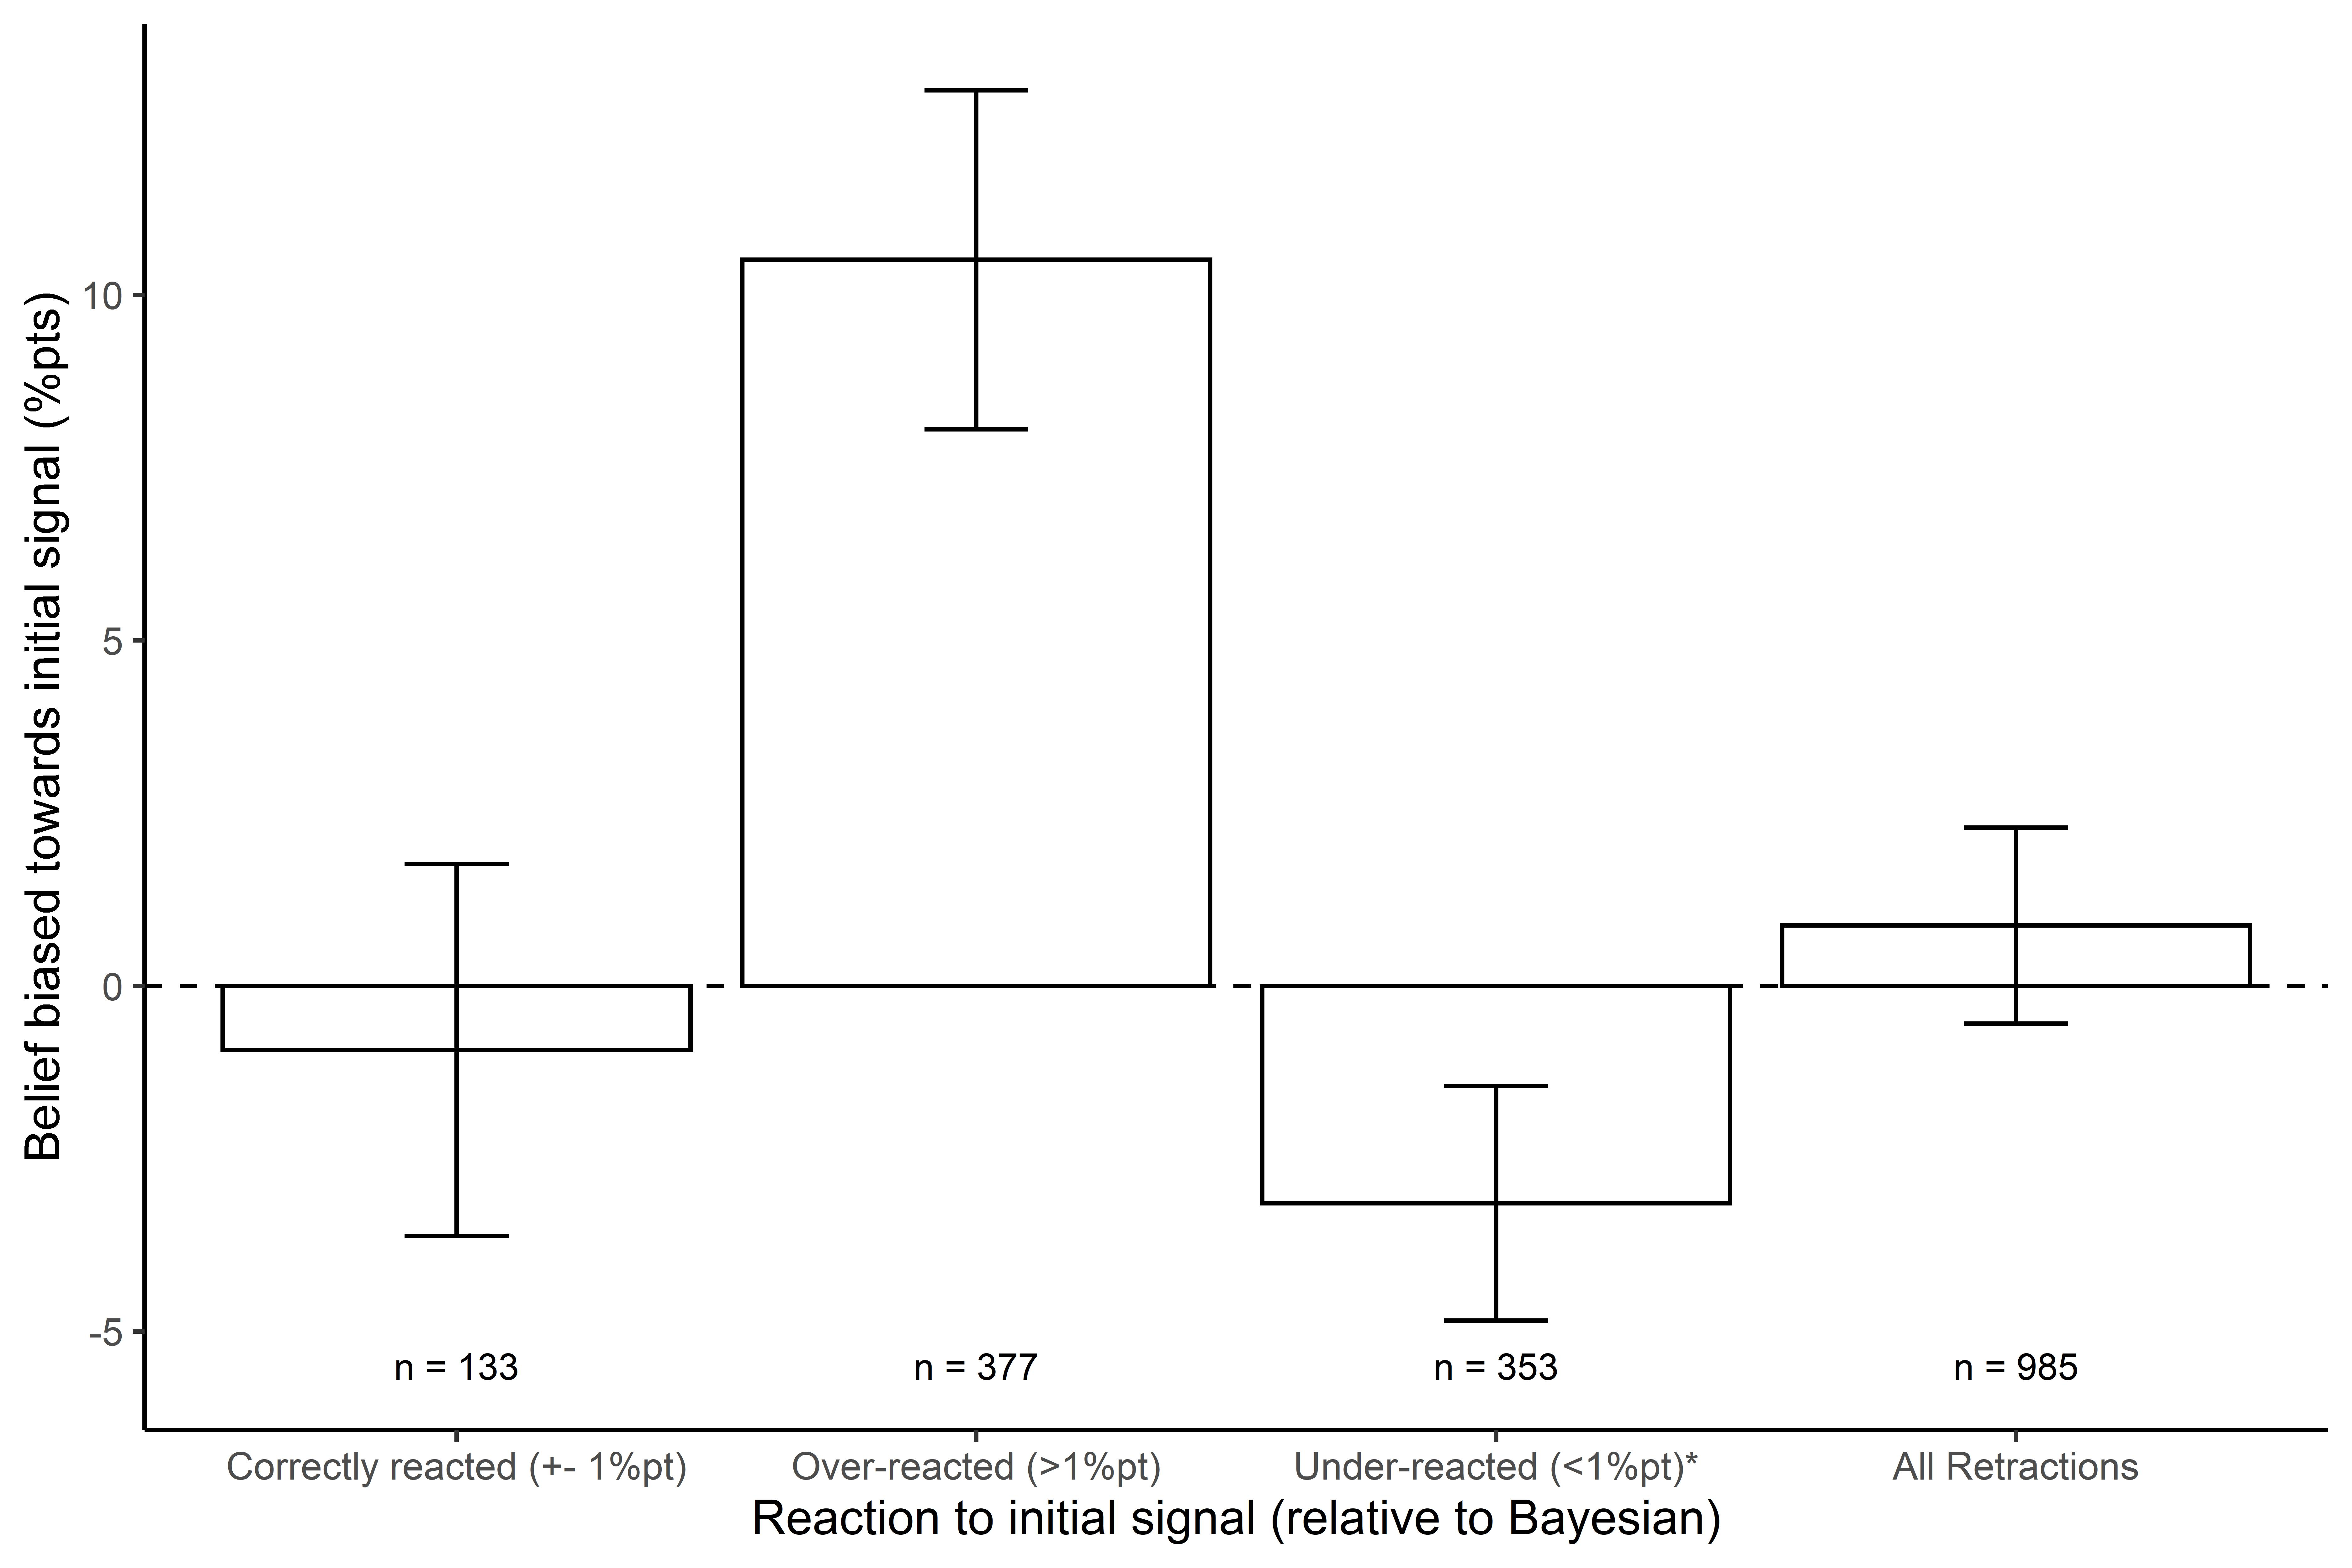
\includegraphics[width = 12cm]{Fig/02_fig_retract_diff_group.jpg}
    \caption{The initial belief update predicts the response to a retraction of that initial signal. *Under-reactions do not include updates in the wrong direction after the initial signal. Including these would lead to a significantly larger difference than shown above.}
    \label{fig:retraction_result_main}
\end{figure}

The results from Table \ref{tab:retractions_main} reveal a further interesting finding. Subjects do not fully forget about their initial prior belief but manage to reduce their initial mistake. The slope of $\beta_1$ is between zero and one, implying that the mistake after the retraction is smaller than the initial mistake. Subjects (attempt to) correct their previous mistake but only do so by about 40\%. To further explain this point, consider the following example. A subject has an initial prior belief of 50\%. He then sees a red ball and reports a belief of 80\%. This reported belief is much higher than the Bayesian posterior which would be 60\%, meaning that the subject over-reported by 20 percentage points. Reporting a posterior of 80\% would have been rational only with a prior of roughly 73\%. In the next step the red ball is retracted. On average, the person does not revert back to 50\% but to roughly 62\%. This can be seen as attempted correction as the subject may have understood he over-reported in the previous round. However, he only corrects about half of his previous mistake. This finding is corroborated when replicating the previous analysis, see Equation \ref{reg:retraction_simple}, but replacing the initial prior with the induced prior. In the above example the induced prior was 73\%. The results are shown in Table \ref{tab:retraction_induced_prior}.

The finding that previous updating explains the reaction to retractions might be expected in many real-world settings with strong motivated reasoning. However, we show that even in a neutral framework without context people are biased when processing retractions. It seems plausible that in many real-world settings that include motivated reasoning, the result would be significantly stronger.


\subsubsection{Robustness Checks} \label{sec:robustness_retractions}

In this section we discuss different robustness checks. We show that our results are robust to different analyses and alternative explanations.

At first we replicate our result using a complimentary analysis introduced by \cite{Goncalves2022}. We compare the beliefs of people who saw a retracted signal to beliefs of people who observed the same exact history excluding the retracted signal. In addition, this method controls for history effects and allows to examine the influence of multiple retractions. To further explain the method we introduce some additional notation. The history of signals for each subject at time $t$ is denoted by $H_t$. This history may for example look like the following: $H_5=(r,r,b,r,retraction)$. If a history contains a retraction we can also define the compressed history which then includes neither the initial signal nor the message of a retraction. This is denoted by $C(H_t)$. Continuing the example from above this would be: $C(H_5)=(r,r,b)$. We can then compare the beliefs of people who saw a retraction to ones who did not. As subjects might observe multiple retractions with an identical compressed history, we control for different retractions histories, $R(H_t)$. In the above example only one red ball was retracted, i.e. $R(H_5)=(r)$. It could be that a subject observes two red retractions and one blue retraction (in this order) which would lead to $R(H_t)=(r,r,b)$. Formally, we estimate the following regression: 
\begin{equation}
    b_t(R|\mathbf{s_1},...,\mathbf{s_t})=\alpha + \beta \cdot F_{R(H_t)} + \gamma \cdot F_{C(H_t)} + \epsilon_t
\end{equation}
where $F_{R(H_t)}$ is a factor variable for all possible retraction histories and $F_{C(H_t)}$ is a factor variable for all compressed histories of signals. Note that up to 3 signals can get retracted for a given subject leading to 14 different combinations of possible orders of retractions, i.e. $F_{H_t(R)}$ has 14 levels.

The results are reported in Table \ref{tab:retraction_compressed_histories}. For nearly all combinations of retracted signals beliefs are not significantly different to beliefs of people who did not see the retracted signal ($\beta\approx0$). Importantly, for a single retraction standard errors are small such that the influence of just one retraction would have been significant if results were similar to the ones reported by \cite{Goncalves2022}. Controlling for time (column 2), by including fixed effects for each round, results in no significant differences for any combination of retracted signals. Only for three retracted signals of the same color (RRR) or (BBB) qualitatively the findings are consistent with the hypothesis of continued influence of retracted information. 

Another method to test for the influence of the initial update is to estimate inference and base-rate use, similar to Equation \ref{eq-reg-inference}. The main difference to before is that the informational value of a retraction signal is not the same for each subject. A subject that inferred a lot more than another subject should also revise their belief more after being told the previous signal was uninformative. For that we calculate a hypothetical information value of a retraction based on the person's initial update. To illustrate, consider the example below. A subject has an initial prior, $p_{t-1}$, and after seeing a regular signal updates to $b_{t-1}$. As mentioned above, after a retraction the rational belief would be $b_t=p_{t-1}$. This fact allows us to calculate a signal such that a Bayesian updater would indeed report $b_t=p_{t-1}$. To do so, we reformulate Bayes rule such that: 
\begin{equation*}
    x =  \frac{p_{t-1} - b_{t-1}\cdot p_{t-1}}{p_{t-1}+b_{t-1}-2\cdot p_{t-1}\cdot b_{t-1}}
\end{equation*}
Having computed a hypothetical signal $x$ we can estimate a regression as in equation \ref{eq-reg-inference}, replacing $p_t$ for $x$:
\begin{equation}
\label{eq:retraction_inference}
    ln(\frac{b_t(R|\mathbf{s_t})}{b_t(B|\mathbf{s_t})}) = \alpha + \beta_1 \cdot ln(\frac{x}{1-x}) + \beta_2 \cdot ln(\frac{p_t(R)}{p_t(B)}) + \epsilon_t
\end{equation}

Result \ref{result_retraction_previous} is further supported by findings from estimating equation \ref{eq:retraction_inference}. The precise estimates can be found in Table \ref{tab:retractions_inference}. It is difficult to compare the regression estimates directly with the ones found in Table \ref{tab:retractions_main} as inference and base-rate use jointly lead to a reported belief. Nonetheless, the results indicate a clear picture similar to results \ref{result_retraction_previous}: The previous update affects how people respond to retractions. Again, people that previously over-reported their belief seem to under-use information ($c<1$) from the retraction and vice versa people that previously under-reported seem to over infer from the retraction ($c>1$). Regressions in columns 2-4 have weaker power due to the smaller sample but the general pattern is the same.

A natural question to consider is whether people can be categorized into types that consistently over- or under-report their belief after a retraction. We do not have enough data per subject to characterize subjects by their reaction to a retraction. However, we can find types based on their updates from regular signals. Two potential methods exist, we can estimate the average inference and base-rate use for each subject or we can calculate the average difference between reported beliefs and Bayesian beliefs. Figure \ref{fig:regular_inf_baserate_type_dist} and \ref{fig:regular_belief_diff_type} show the distribution of types for the two different methods. It is important to note that while the type distributions based on inference and base-rate use have a relatively low variance, the variance for each subject is significant. This indicates that each individual belief report for a given subject is quite noisy. To find out whether the subject type can explain people's biased reaction to retractions we estimate several regressions, including the initial belief update, the average over-report of beliefs, as well as average inference and base-rate use. Formally, we estimate the following regression, similar to Equation \ref{reg:retraction_simple}:
\begin{equation*}
    b_t-p_{t-1}=\alpha 
    + \beta_1 \cdot (b_{t-1}-B_{t-1})
    + \beta_2 \cdot \Bar{o}*I(s_{t-1})
    + \beta_3 \cdot (\hat{c}-1)*I(s_{t-1})
    + \beta_4 \cdot (\hat{d}-1)*I(s_{t-1})
    + \epsilon_t
\end{equation*} 
where $\Bar{o}$ denotes the average over-report of beliefs adjusted for the signal direction: $\sum_{t\in R}(b_t-B_t)*I(s_t)$ and $R$ is the set of all regular updating rounds. In addition we run a further regression check:
\begin{equation*}
    b_t-p_{t-1}=\alpha 
    + \beta_1 \cdot (b_{t-1}-B_{t-1})
    + \beta \cdot F(\text{type})
    + \epsilon_t
\end{equation*}

where 'type' refers to a grouping of subjects by their response to regular signals. We group subjects into different categories based on their reaction to the majority of signals (at least 5 out of 9).

The results, reported in Table \ref{tab:retractions_types}, clearly show that the update from the initial uncertain signal remains an important explanatory variable which is not explained by any classification of types, i.e. in all four columns. In fact, in column (1) $\beta_2$ is negative meaning that as subjects consistently over-report they are better at reacting to retractions even when the initial update was an over-reaction. This is confirmed by the negative parameter for average inference in column (2). Furthermore, the grouping of subjects based on the majority of reactions to regular signals are not predictive of the reaction to retractions. This further corroborates the fact that the initial update predicts the response to a retraction. In general, the analysis of subject types shows that people's types explain part of the bias with retraction updates but they predict much less than last round's over-report.\footnote{This is further supported by the fact that excluding last rounds update in the regression leads an R squared nearly equal to zero with just the average over-report remaining.} In summary, we find that the initial update is the main predictor of the reaction to a retraction.

A further question to consider is whether subjects are reporting 'incorrect' posteriors after the retraction to correct for a previous mistake they might have made. Bayesian posteriors in our setting are based on the idea that subjects update their beliefs sequentially after each new signal they observe. It might be that instead subjects realised they made a mistake before and are trying to correct this after the retraction by reporting a belief that is not equal to the initial prior belief. A simple test is to include a variable in regression \ref{reg:retraction_simple} that controls for the difference between the reported belief and the Bayesian belief before observing the uncertain signal. Formally, we then estimate the following regression:
\begin{equation}
    b_t(R|\mathbf{s_{t-1}}, \mathbf{r_t})-p_{t-1}(R)=\alpha + 
    \beta_1 \cdot (b_{t-1}(R|\mathbf{s_{t-1}})-p_{t-1}(R|\mathbf{s_{t-1}})) +
    \beta_2 \cdot (b_{t-2}(R|\mathbf{s_{t-2}})-p_{t-2}(R|\mathbf{s_{t-2}})) +
    \epsilon_t
\end{equation}

We find that $\beta_1$ remains significantly different to zero, as reported in Table \ref{tab:retractions_explanatory} column (1). In fact, the coefficient of $\beta_1$ is larger than in the original regression result, see Table \ref{tab:retractions_main}. $\beta_2$ is also significantly different from zero and negative. It seems that while the previous mistake has a small influence on the response to a retraction, the effect is in the opposite direction. Subjects are certainly not misreporting beliefs on purpose to offset an initial mistake. If anything, the opposite is true.

A final question is whether the way information is displayed to the subjects could influence the results. In particular, it could be that showing subjects their previously reported belief anchors them to that number. To test for the effect of our experimental design we varied the information display in  2 additional treatments. In treatment 2 we do not display the previously reported belief and in treatment 3 we hide the history of signals, only displaying the most recent signal and in case of verifications also the uncertain initial signal. Again, we estimate a similar regression to before, now including variables for the 2 additional treatments and their interaction with the initial belief update. In Table \ref{tab:retractions_explanatory} column (2) we report the effect information display. In general, information display does not affect to what extent people changed their beliefs. 

In summary, none of the natural alternative factors seem to fully explain subject's bias when responding to a retraction. The difference between the initially reported belief and the Bayesian posterior remains the most important factor predicting how people respond to the retraction of the same signal.


\subsubsection{Retractions vs Opposite New Information}

We have shown so far that people are biased in a predictable way when confronted with a retraction. This finding is also robust to a large number of alternative explanations. However, one may wonder if retractions are different to regular signals. In this section we analyzes the differences between opposite new information and retractions of previous information. Retractions are informationally equivalent to showing an opposite colored ball. To illustrate, consider the following example. A subject has a prior belief of 50\% and sees a red ball. He updates his belief to 60\%. Now two signals are informationally equivalent, a retraction of the red ball and a new blue ball. After both signals the subject should update his belief to 50\%. This is also the case for any other prior the subject may have. 

For the analysis we pool all observations for which subjects receive two consecutive uncertain signals of opposite color. This allows for a simple comparison between retractions and opposite colored signals, similar to before. We have already shown that there is no significant difference in in beliefs before and after a retracted signal. We replicate this analysis but with opposite colored balls. The result can be seen in Figure \ref{fig:retract_vs_opposite}. We find that reactions to opposite colored balls are significantly different to belief updates after a retraction. Subjects substantially over-react to the second ball and end up with a posterior belief significantly different to their initial prior.

\begin{Result}
    People react differently to retractions of a past signal versus new opposite information.
\end{Result}

\begin{figure}
    \centering
    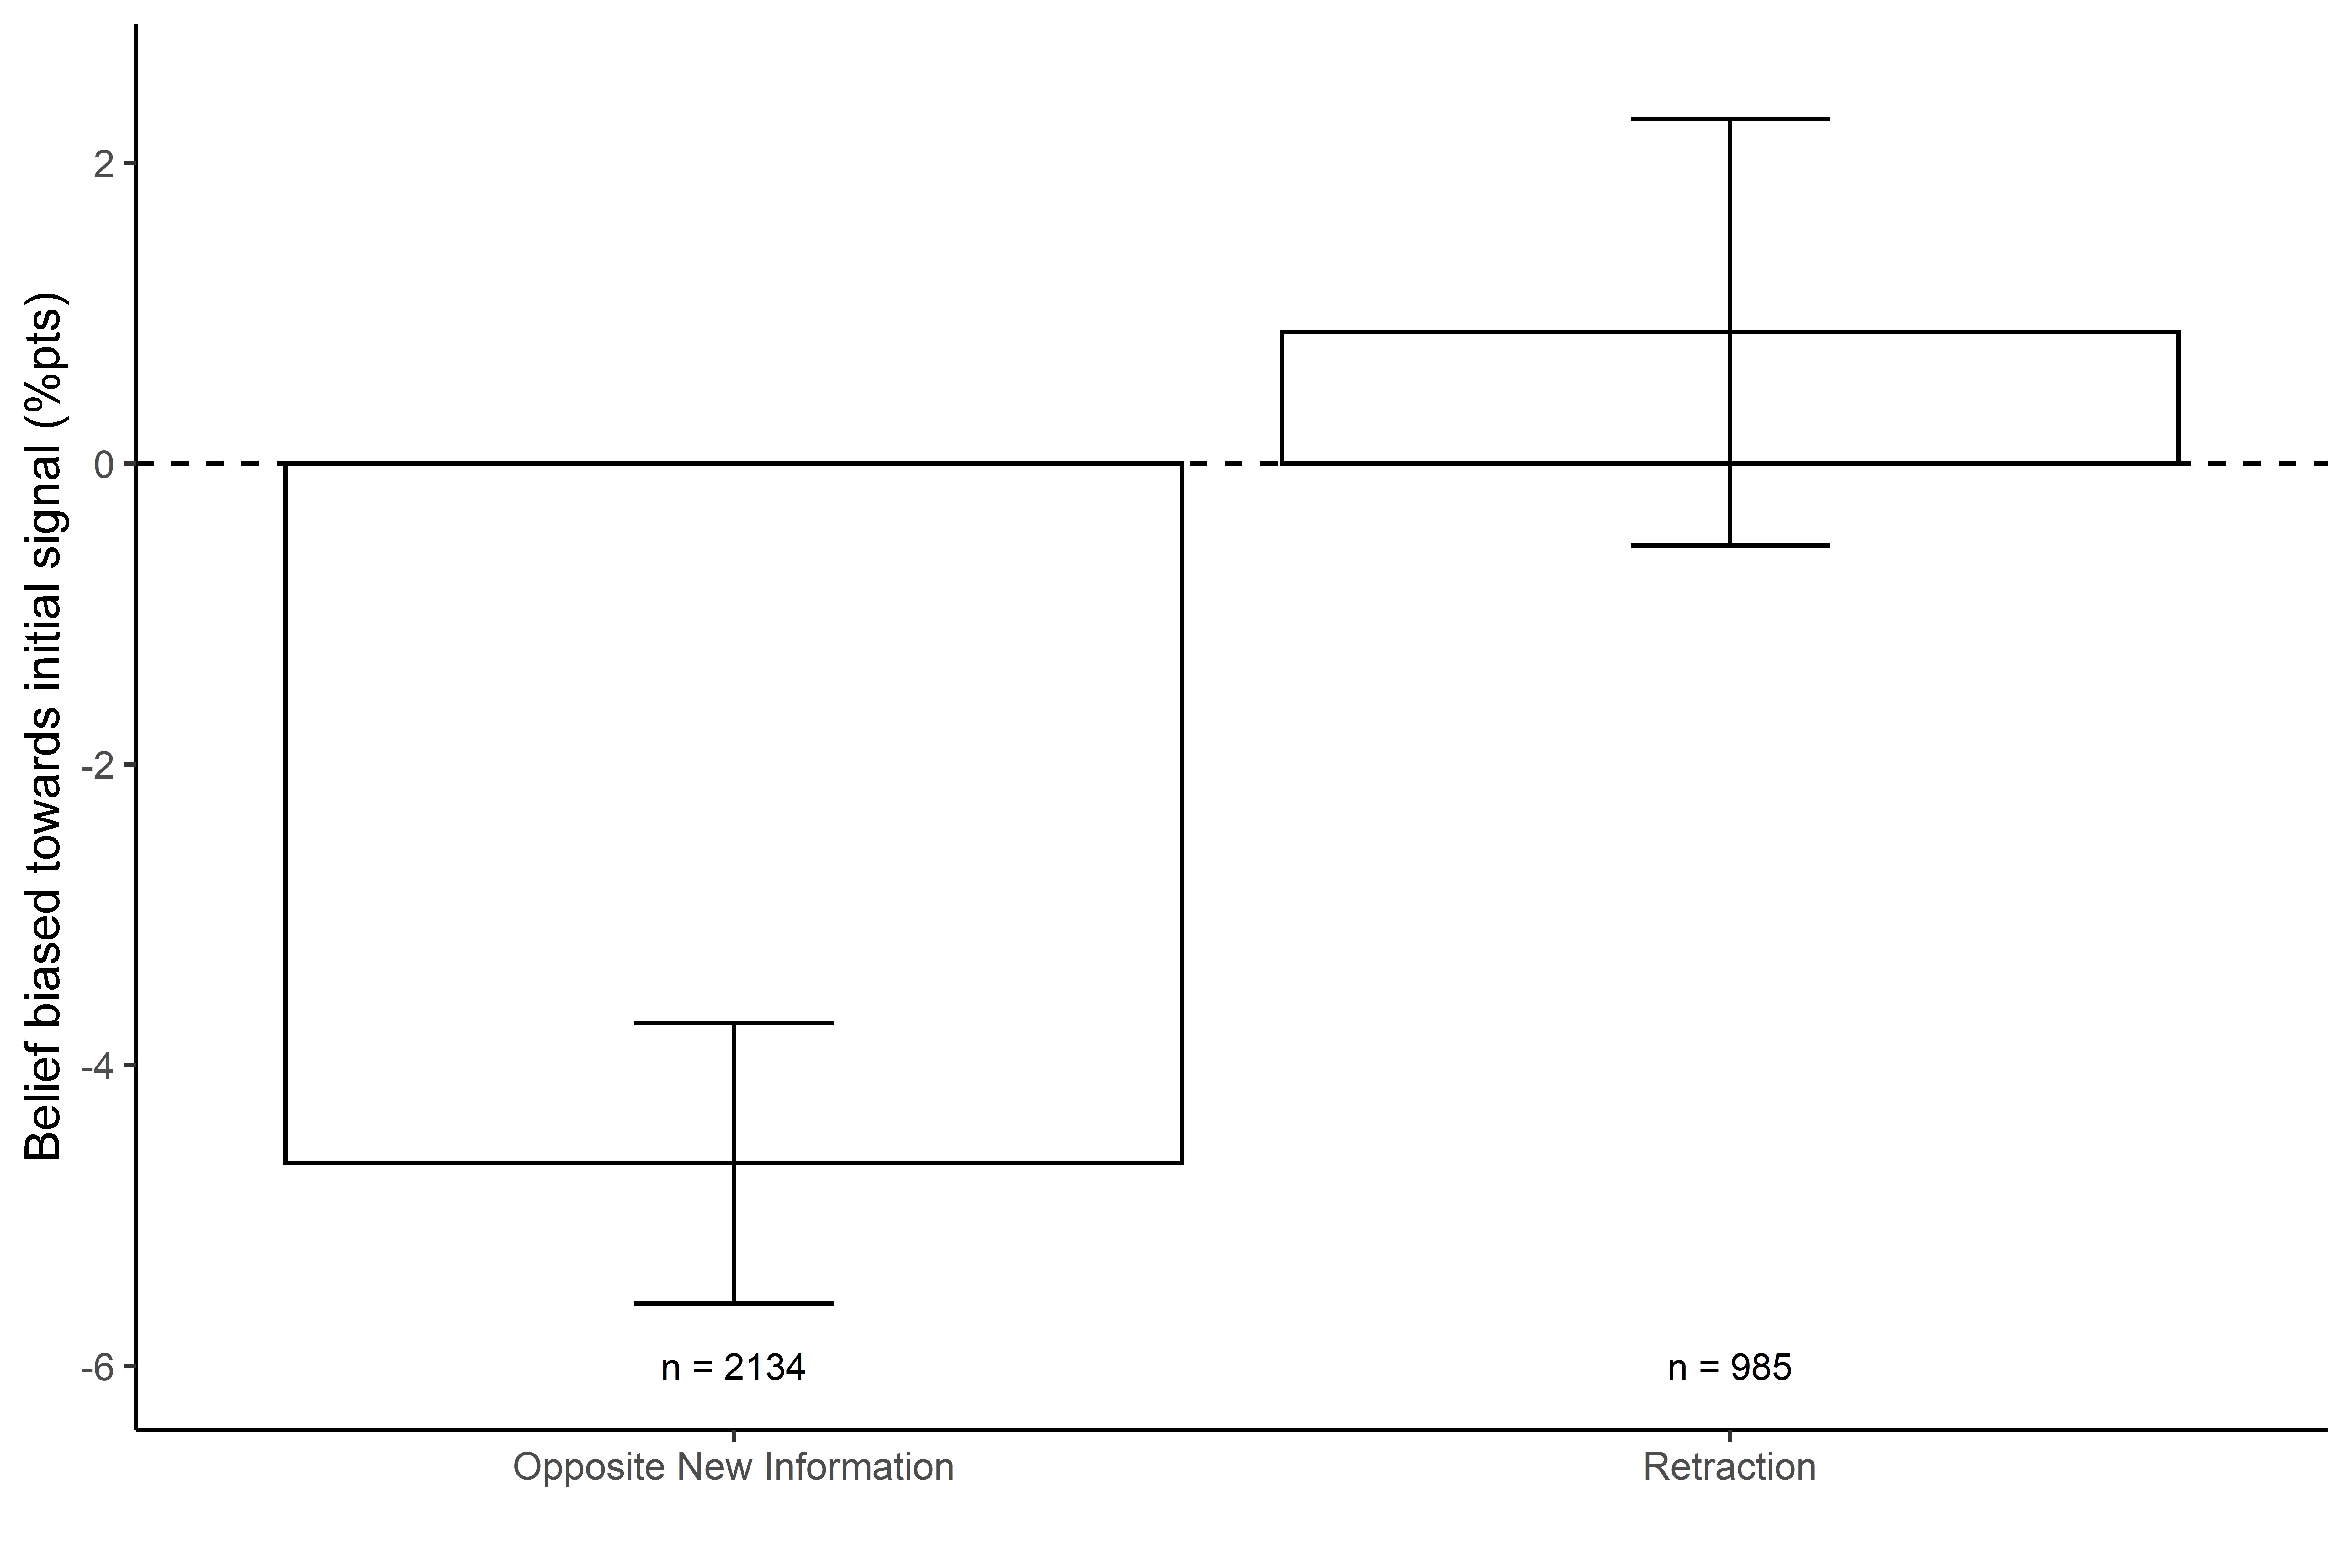
\includegraphics[width=10cm]{Fig/02_fig_retract_diff_vs_opposite_ball_all.jpg}
    \caption{Retractions versus Opposite Signals. Comparison of mean belief differences to the initial prior belief.}
    \label{fig:retract_vs_opposite}
\end{figure}

In addition we test for differences between opposite new information and retraction of past information by comparing the exact histories of previous signals. This method is very similar to the analysis we introduced in section \ref{sec:robustness_retractions} and based on \cite{Goncalves2022}. We compare reported beliefs with fixed effects for each possible history to isolate the difference between two opposite signals versus a retraction of a past signal. To illustrate, consider the history $H_4=(r,b,r,retraction)$. For the purpose of comparing retraction to opposite new information we introduce the opposite signal history, which in the example above is given by: $O(H_t)=(r,b,r,b)$. Formally, we estimate the following regression:
\begin{equation}
    b_t(R|\mathbf{s_1},...,\mathbf{s_t})=\alpha + \beta_1 \cdot r_t + \beta_2 \cdot s_t + \beta_3 \cdot r_t*s_t + \gamma \cdot F_{O(H_t)} + \epsilon_t
\end{equation}
where $r_t$ denotes a retraction round, $s_t$ the direction of the retracted signal and $F_{O(H_t)}$ denotes the fixed effects for each history where retractions are coded identical to opposite signals. $\beta_3$ is the main coefficient of interest. The results are reported in Table \ref{tab:retract_vs_ball}. The findings are in line with the graphical representation in Figure \ref{fig:retract_vs_opposite}, retractions are different to opposite new information. People over-react to opposite new information and end up with a belief different to their initial prior.


\subsection{Confirmations}

\subsubsection{Main Results}

In this section we turn to the analysis of confirmations. A confirmation is a signal telling the subject the previous signal realisation was generated by the informative signal, $\pi_I$. As explained above a rational subject should forget about the uncertain signal and update from his initial prior using $\pi_I$. The initial update should not influence the belief after a confirmation. Formally, the Bayesian posterior after a confirmation is given by Equation \ref{eq-confirmation}.

As the initial step we compare the simple average belief changes to the average Bayesian changes.\footnote{We exclude observations where people rationally should not change their belief in response to the initial signal. These are subjects who for example reported a belief of 100\% and then see another red ball.} Figure \ref{fig:confirm_change} shows the result. While people on average slightly over-reacted to the initial signal, beliefs are lower than Bayesian after the confirmation of the initial signal. Subjects clearly under-react to the confirmation. In the following we analyse this question further. One additional point to notice from this simple comparison of average belief changes is that people reacted stronger to the initial signal (on average ~10\% points) than the confirmation thereof (on average ~8\% points). Given the informativeness of the two signals in our design, if subjects were fully rational we would see the opposite pattern.

\begin{figure}[!htb]
    \centering
    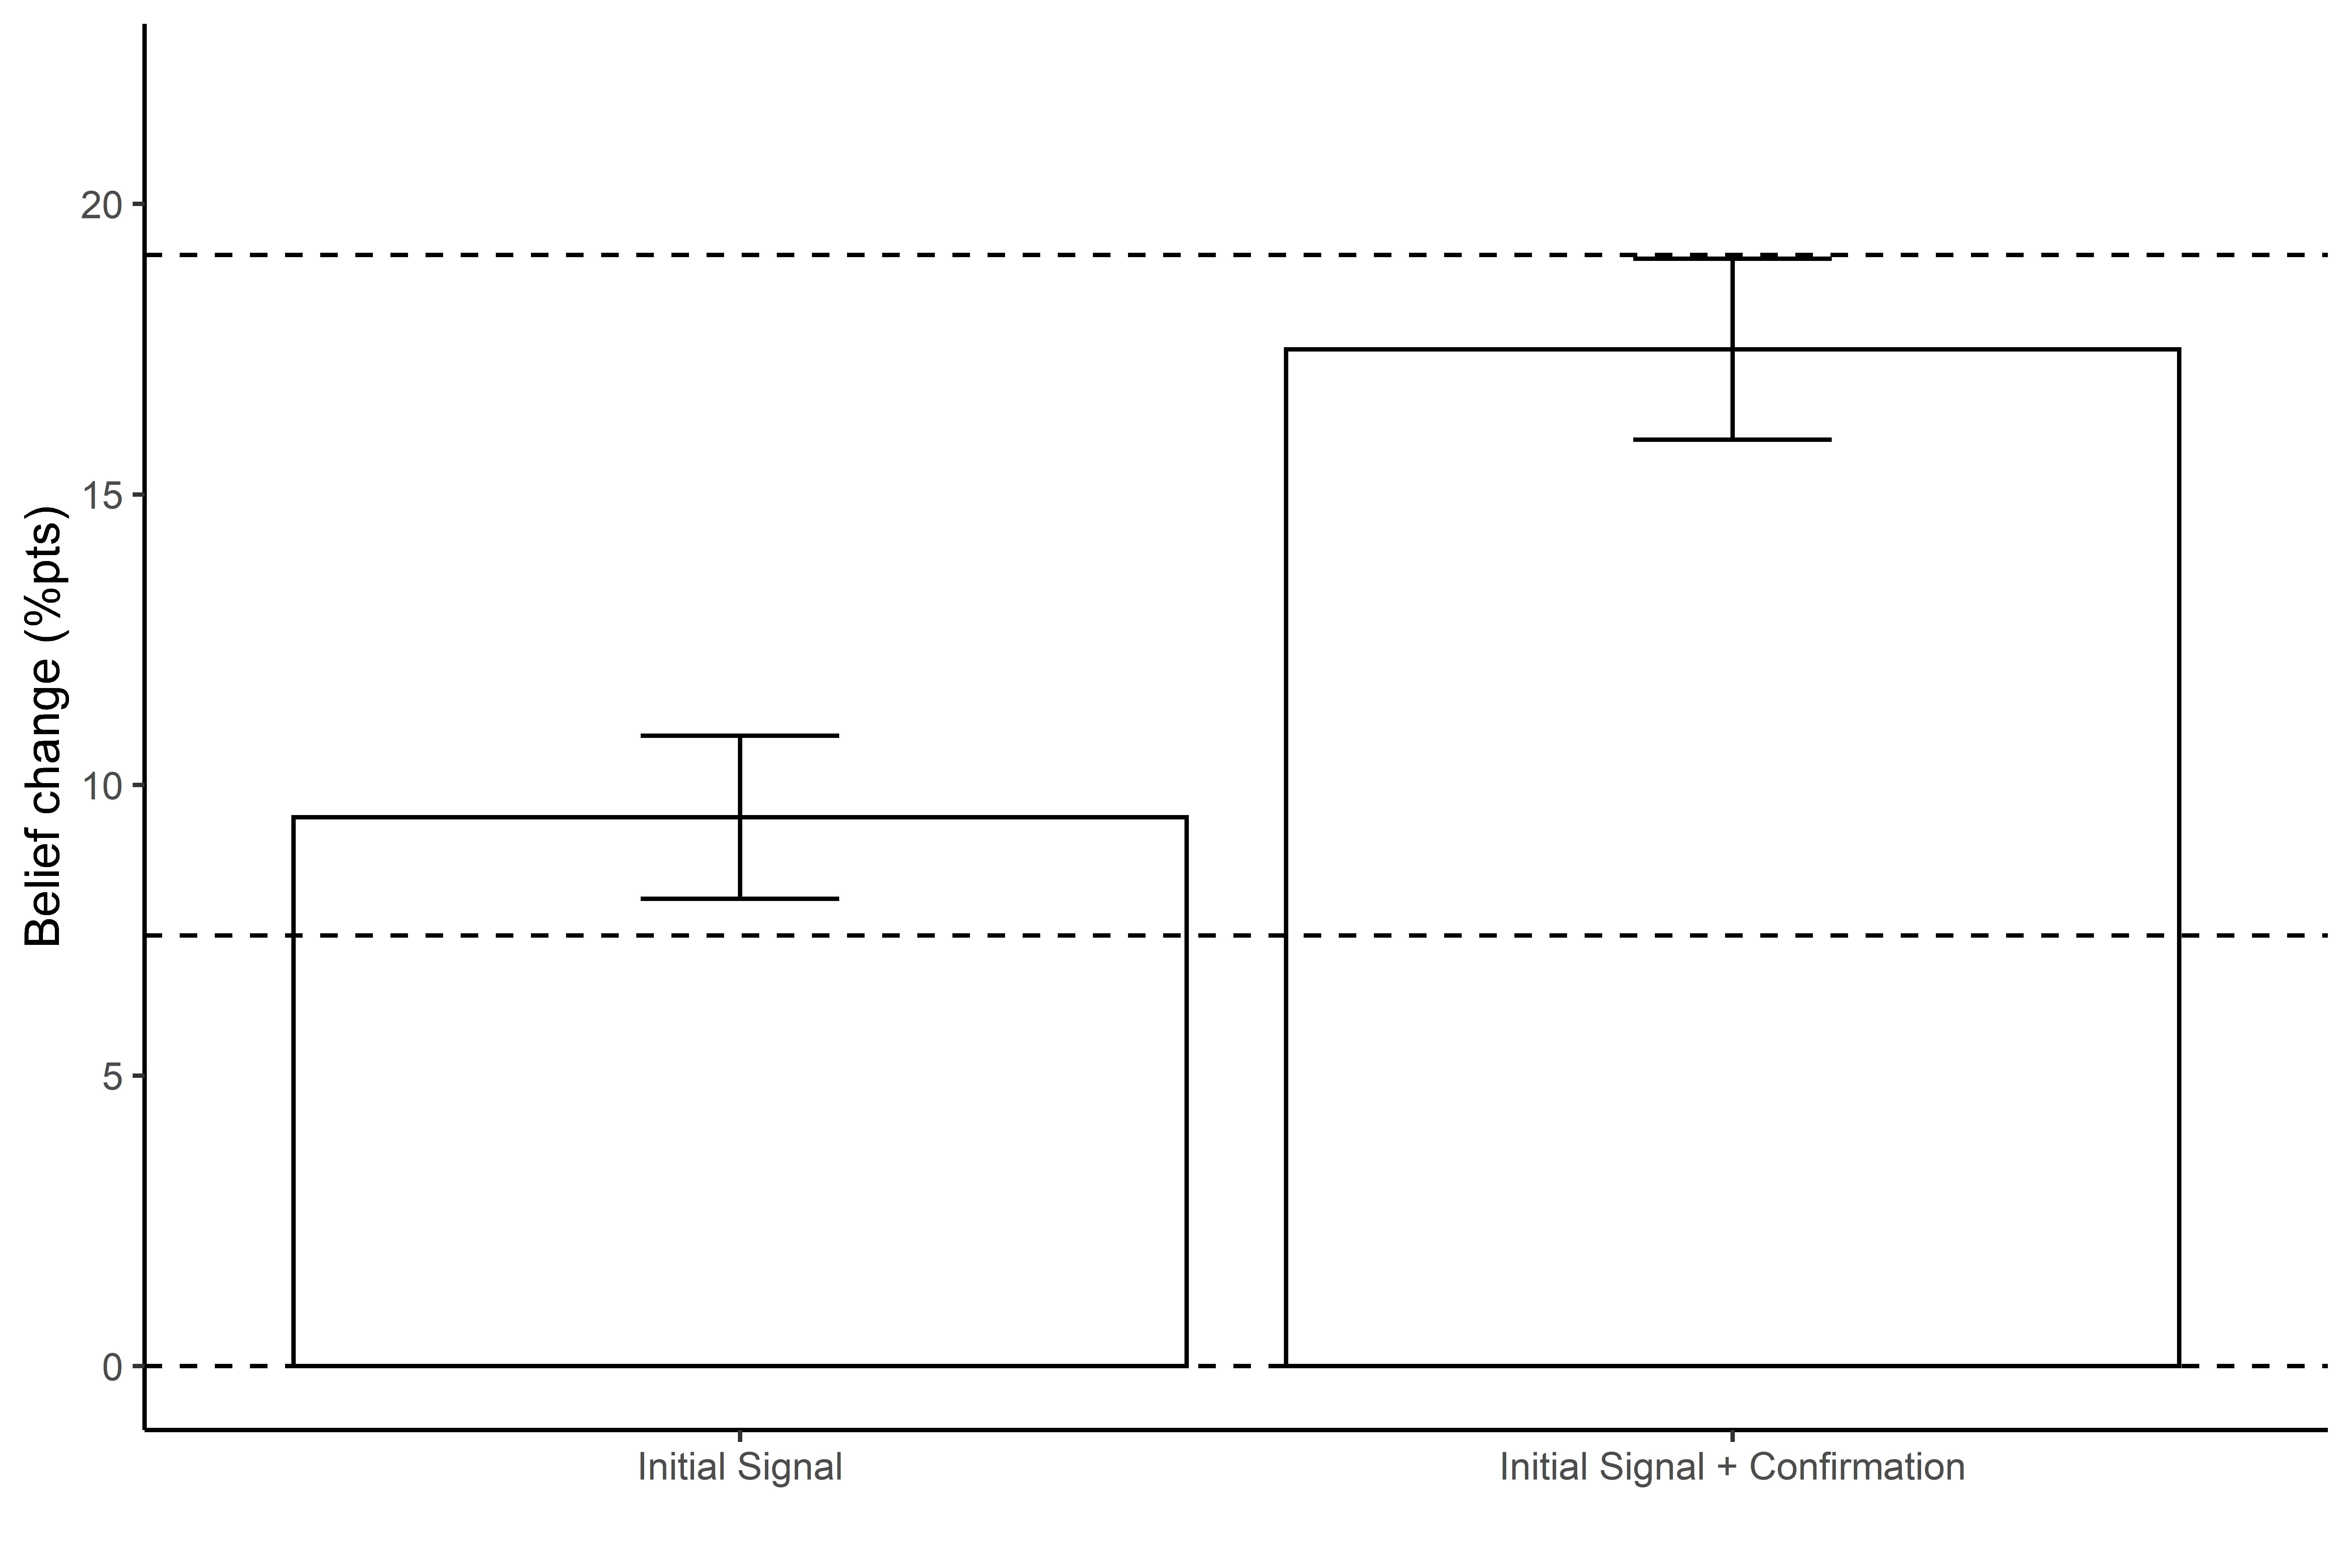
\includegraphics[width=10cm]{Fig/02_fig_confirm_change.jpg}
    \caption{Reaction to confirmation signals. The dashed line at roughly 7.5 indicates the average Bayesian response to an uncertain signal. The dashed line at roughly 19 indicates the average Bayesian response to the confirmed signal.}
    \label{fig:confirm_change}
\end{figure}

A better method to study the influence of confirmations is to test how people react to the confirmation of a previous signal based on their initial reaction. To do so, we employ a similar methodology as with the analysis of retractions. Again, we compare absolute belief differences between the Bayesian posterior and the reported belief, taking into account the initial update:

\begin{equation}
\label{reg:confirmation_simple}
    b_t(R|\mathbf{s_{t-1}},\mathbf{c_t})-p_{t}(R|\mathbf{s_{t-1}},\mathbf{c_t})=\alpha + \beta_1 \cdot (b_{t-1}(R|\mathbf{s_{t-1}})-p_{t-1}(R|\mathbf{s_{t-1}}))*I(s_{t-1})+\epsilon_t
\end{equation}

The results are reported in Table \ref{tab:confirmation_main}. We find that, as with retractions, $\beta>0$, suggesting that subjects misreport their beliefs systematically after confirmations. The initial update relative to Bayesian strongly predicts how people respond to a confirmation of the same signal. Moreover, $\alpha$ is smaller than zero, indicating that subjects under-reacted to confirmations in general. The findings are robust to controlling for wrong initial updates and using an alternative Bayesian posterior as the benchmark (as shown in columns 2 and 3). We summarize the result below.

\begin{Result}
\label{res:confirm}
Subjects systematically under-react to a confirmation. Moreover, their initial reaction strongly predicts the belief report after the confirmation.
\end{Result}

As with retractions we can visualize reported beliefs for different groups of subjects, those that initially under-reacted, reacted correctly, and (slightly) over-reacted (see Figure \ref{fig:confirm_diff_restricted}). There are further groups and the complete picture is attached in the appendix, see Figure \ref{fig:confirm_diff_complete}. Consistent with the results presented above, we find that subjects systematically under-react to confirmations. Even the group of subjects that initially reacted in a Bayesian way to the uncertain information under-reacted to the confirmation thereof. Only those subjects that initially over-reacted end up with a belief that is approximately Bayesian. 

\begin{figure}
    \centering
    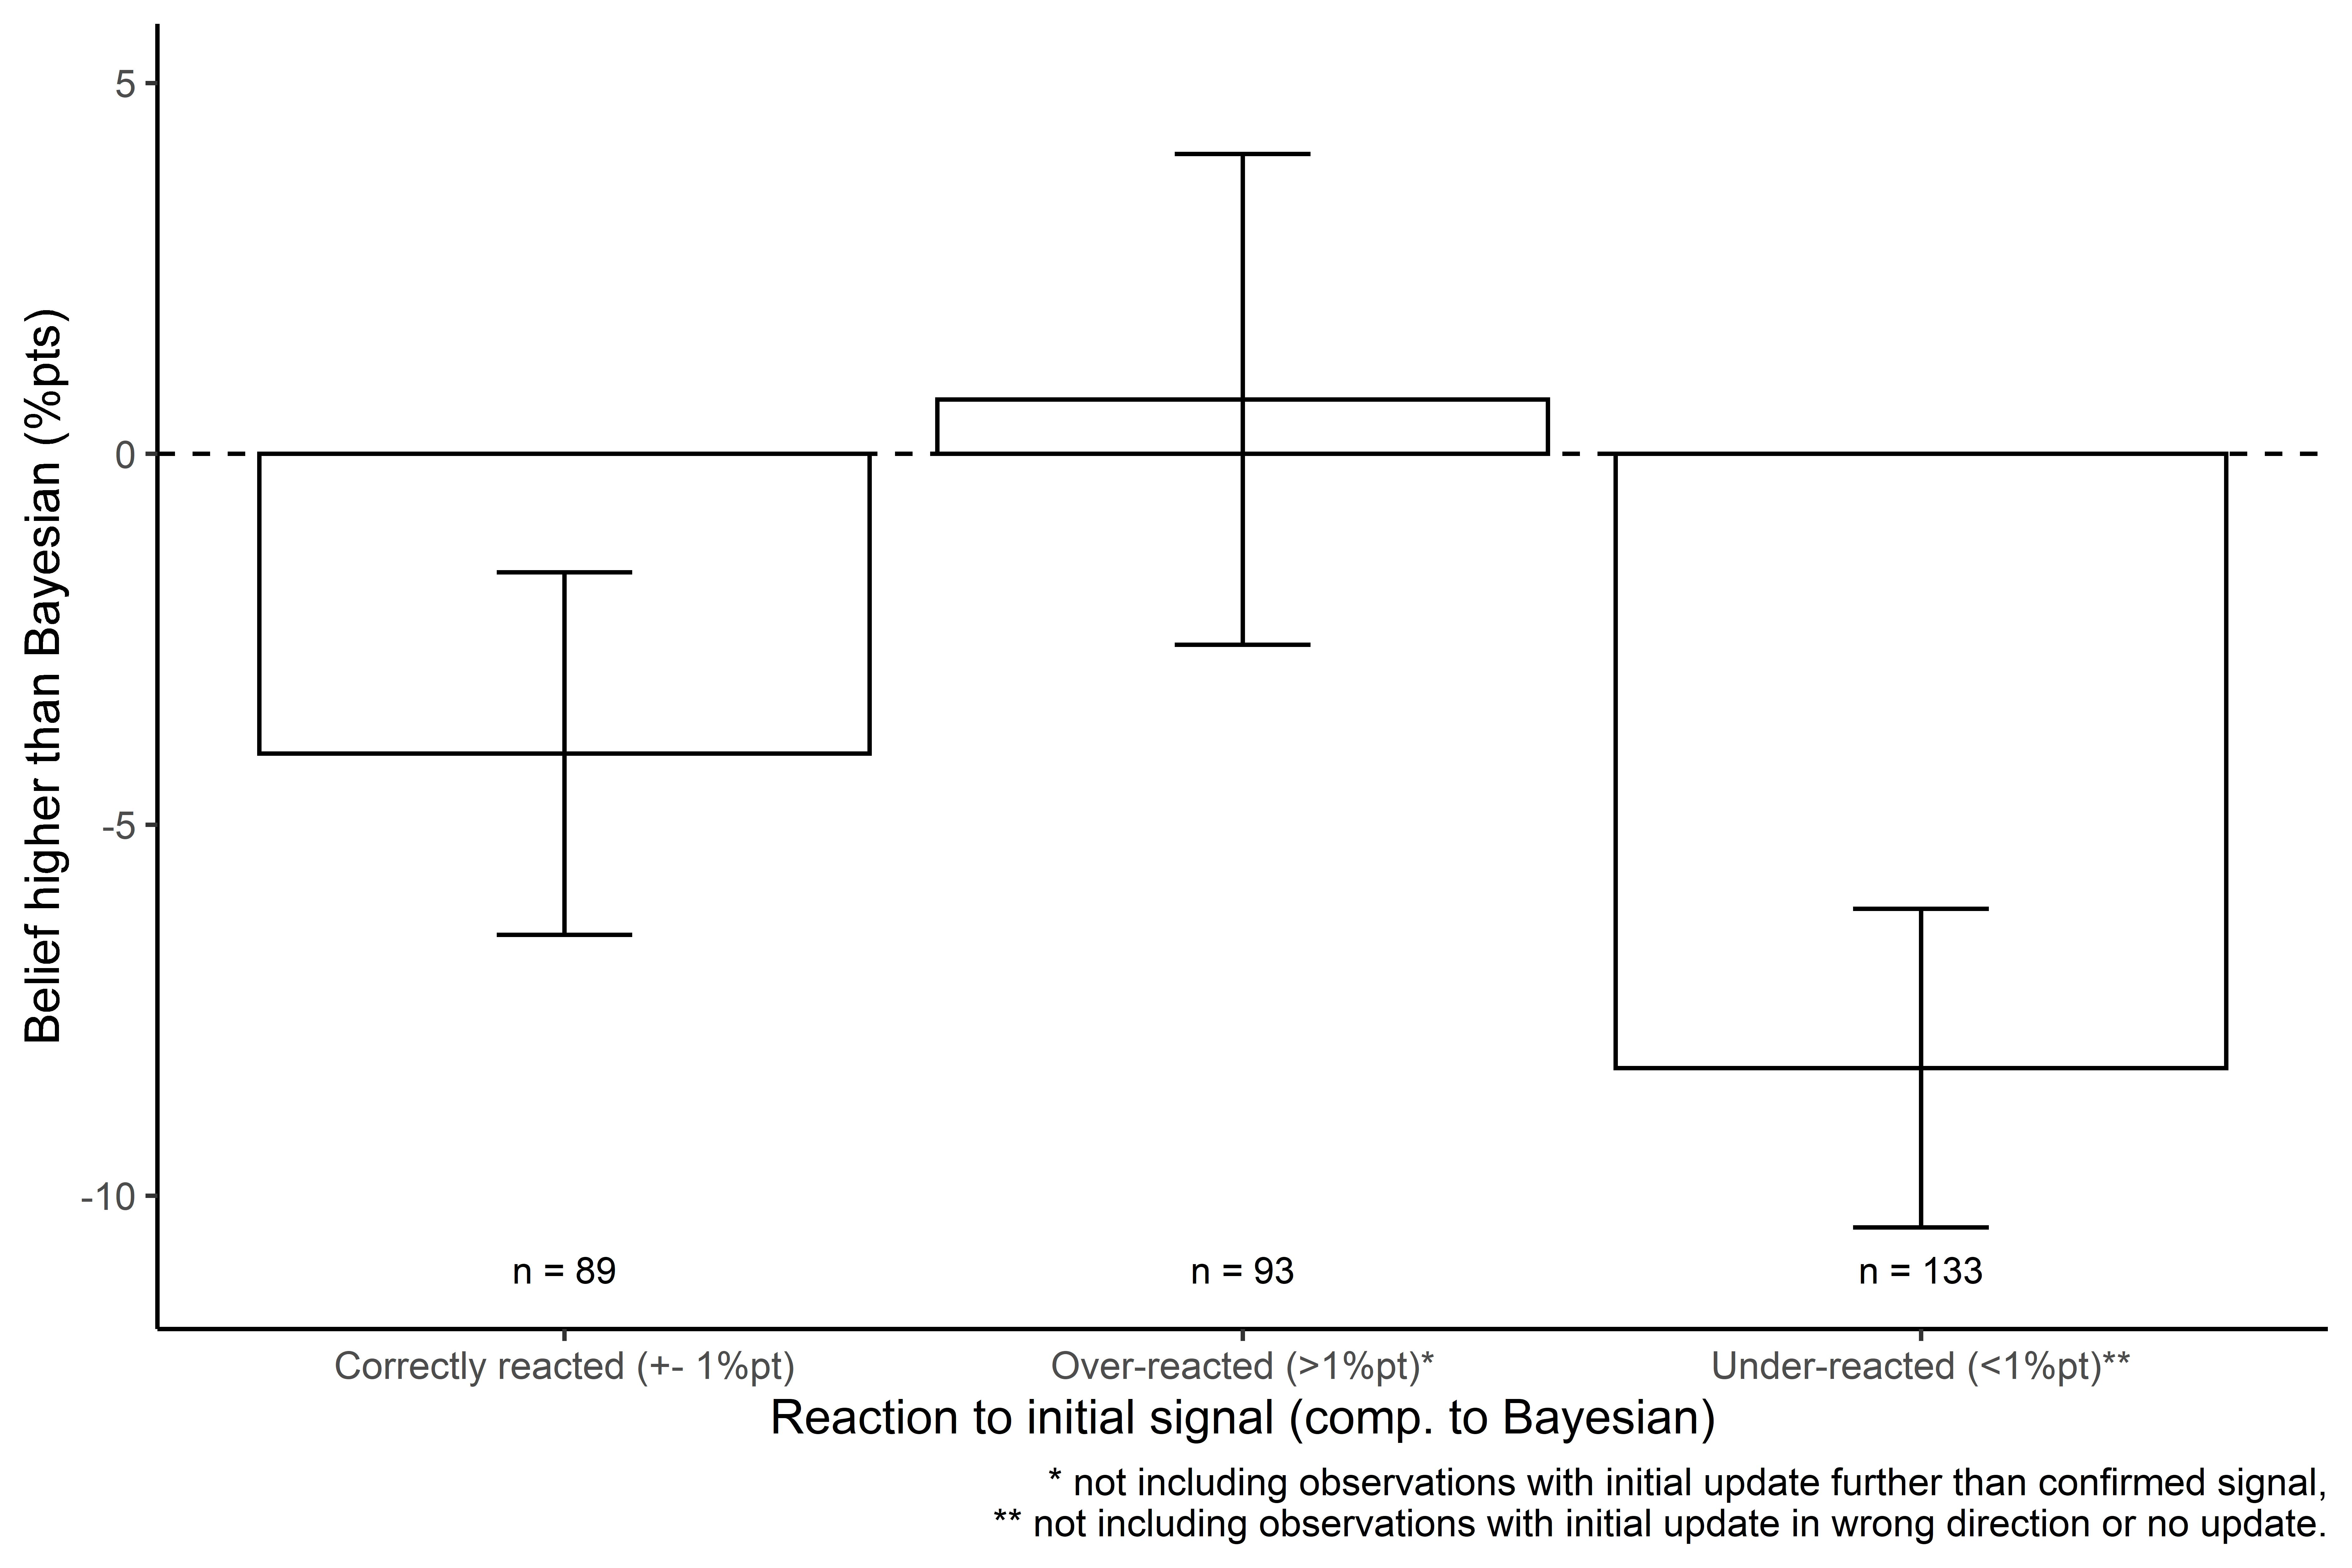
\includegraphics[width=12cm]{Fig/02_fig_confirm_diff_restricted.jpg}
    \caption{Influence of the initial reaction on beliefs after a confirmation.}
    \label{fig:confirm_diff_restricted}
\end{figure}


\subsection{Ex-ante Verifications of Information}

In this section we turn to the analysis of the third research question: What is the effect of checking information ex-ante? We analyze 1) whether people react differently to ex-ante verifications in general, as compared to ex-post checks, and 2) whether beliefs are more dispersed after retracted signals than equivalent uninformative signals.

\subsubsection{Uninformative Signals}
An uninformative signal in our design is a combination of a regular signal (i.e. the color of a ball) and the additional information that this ball is uninformative (i.e. it did not come from the randomly selected urn). A rational subject should not update their belief and report the same posterior belief as in the previous round. 

We find that a large number of subjects correctly reports the same belief as previously. However, some subjects update their belief towards the color of the signal shown, despite this being uninformative. That leads to, on average, a small but significant difference in beliefs towards the uninformative signal color. The result is shown in Figure \ref{fig:uninformative_vs_retract}. While we do not find such an effect on average for retracted signals, the average belief change for uninformative signals is not significantly different to retracted signals at the 5\% level.

\begin{figure}[!htb]
    \centering
    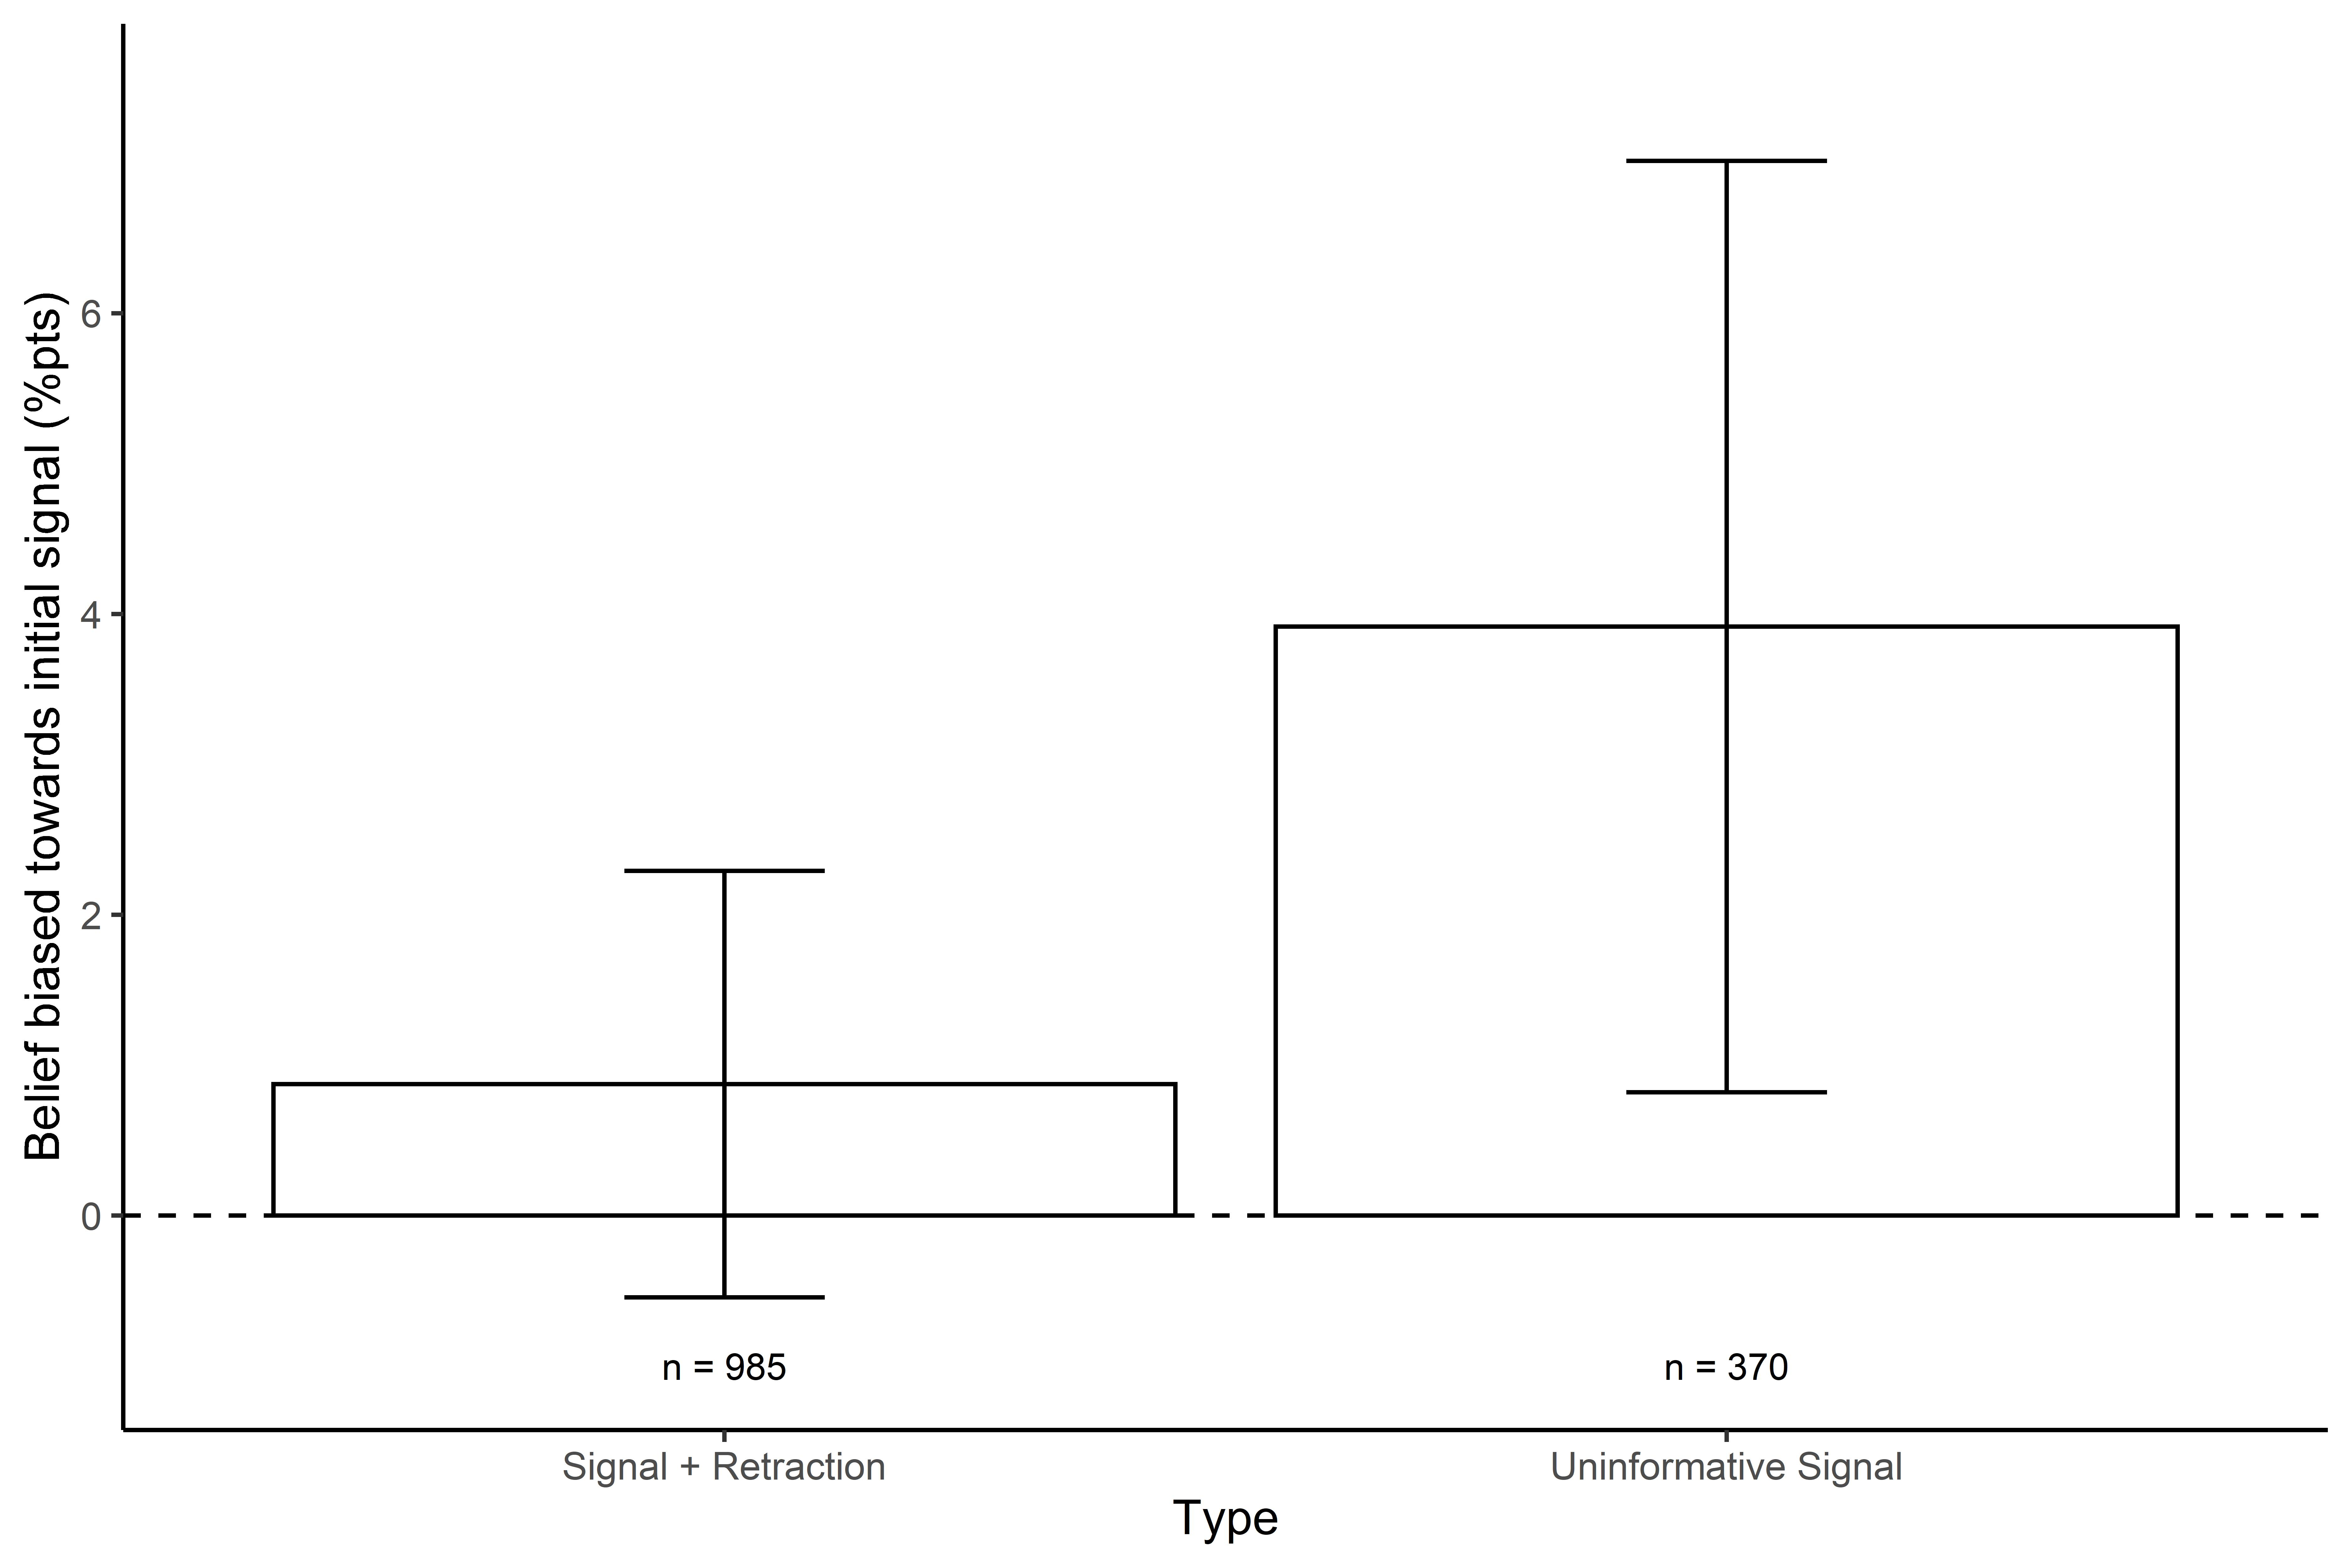
\includegraphics[width=10cm]{Fig/02_fig_retract_vs_uninformative.jpg}
    \caption{Average difference between prior and posterior belief following an uninformative/retracted signal, adjusted for the signal direction.}
    \label{fig:uninformative_vs_retract}
\end{figure}

To clearly compare uninformative and retracted signals we compare beliefs after retractions to beliefs after uninformative signals for each exact history of previously observed signals. Similar to before, we introduce some additional notation for ease of explanation. For any history $H_t$ we can define the aggregate history $A(H_t)$. Consider the example where a subject observed some history of signals where the red ball from period 4 ball is retracted in period 5, $H_5=(r,r,b,r,\text{retract})$. The aggregated history is then given by: $A(H_5)=(r,r,b,r_\text{uninf.})$. Furthermore, as before, we control for any combination of previous uninformative signals through $U(H_t)$. In the example above this would be $U(H_5)=(r_\text{uninf.})$. Formally, we estimate the following regression:
\begin{equation}
    b_t(R|\mathbf{s_1},...,\mathbf{s_t})=\alpha + \beta \cdot F_{U(H_t)} + \gamma \cdot F_{A(H_t)} + \epsilon_t
\end{equation}
where $F_{U(H_t)}$ is a factor variable for all possible combinations of uninformative signals and $F_{A(H_t)}$ is a factor variable for all 'aggregated' histories, i.e.  histories with retracted signals are coded the same as histories with uninformative signals. Any coefficient $\beta$ that is non-zero indicates differences between uninformative signals and retracted signals. The results are reported in Table \ref{tab:uninformative_vs_retractions}. We find that for a single uninformative signal (with color red or blue) beliefs are not significantly different to beliefs after an equivalent retraction. Only with multiple uninformative signals some differences emerge. However, these are based on small sample sizes and the significance of certain parameters should be treated with caution.

A second question we can analyse is the dispersion of beliefs for retracted signals in comparison to uninformative signals. Ideally, all people would return to their initial prior after a retracted signal. We have previously shown that this is not the case. Comparing the spread in beliefs with uninformative signals provides a clear benchmark. To specific points are interesting to note, 1) the number of people correctly reporting their initial prior and 2) the variance of beliefs. We analyze those two questions for one and multiple consecutive retractions/uninformative signals, irrespective of the color associated with the signal. Ultimately, we compare the initial starting prior to the belief after one, two or three consecutive retractions/uninformative signals. For a rational subject this difference should be zero.

Figure \ref{fig:variance_retract_uninformative} provides a clear overview of the differences between retractions and uninformative signals. The number of people correctly returning to their initial belief is lower than with uninformative signals after any number of retractions. With every additional retracted signal fewer people correctly return to their initial prior. After three consecutive retracted signals the variance of beliefs is substantially higher than after three uninformative signals (Var: 7.1\%pts vs. 4.4\%pts). This implies that, while there is no evidence in our data for a continued influence of retracted information, multiple retracted signals lead to substantially biased beliefs for the vast majority of subjects.

\begin{figure}[!htb]
    \centering
    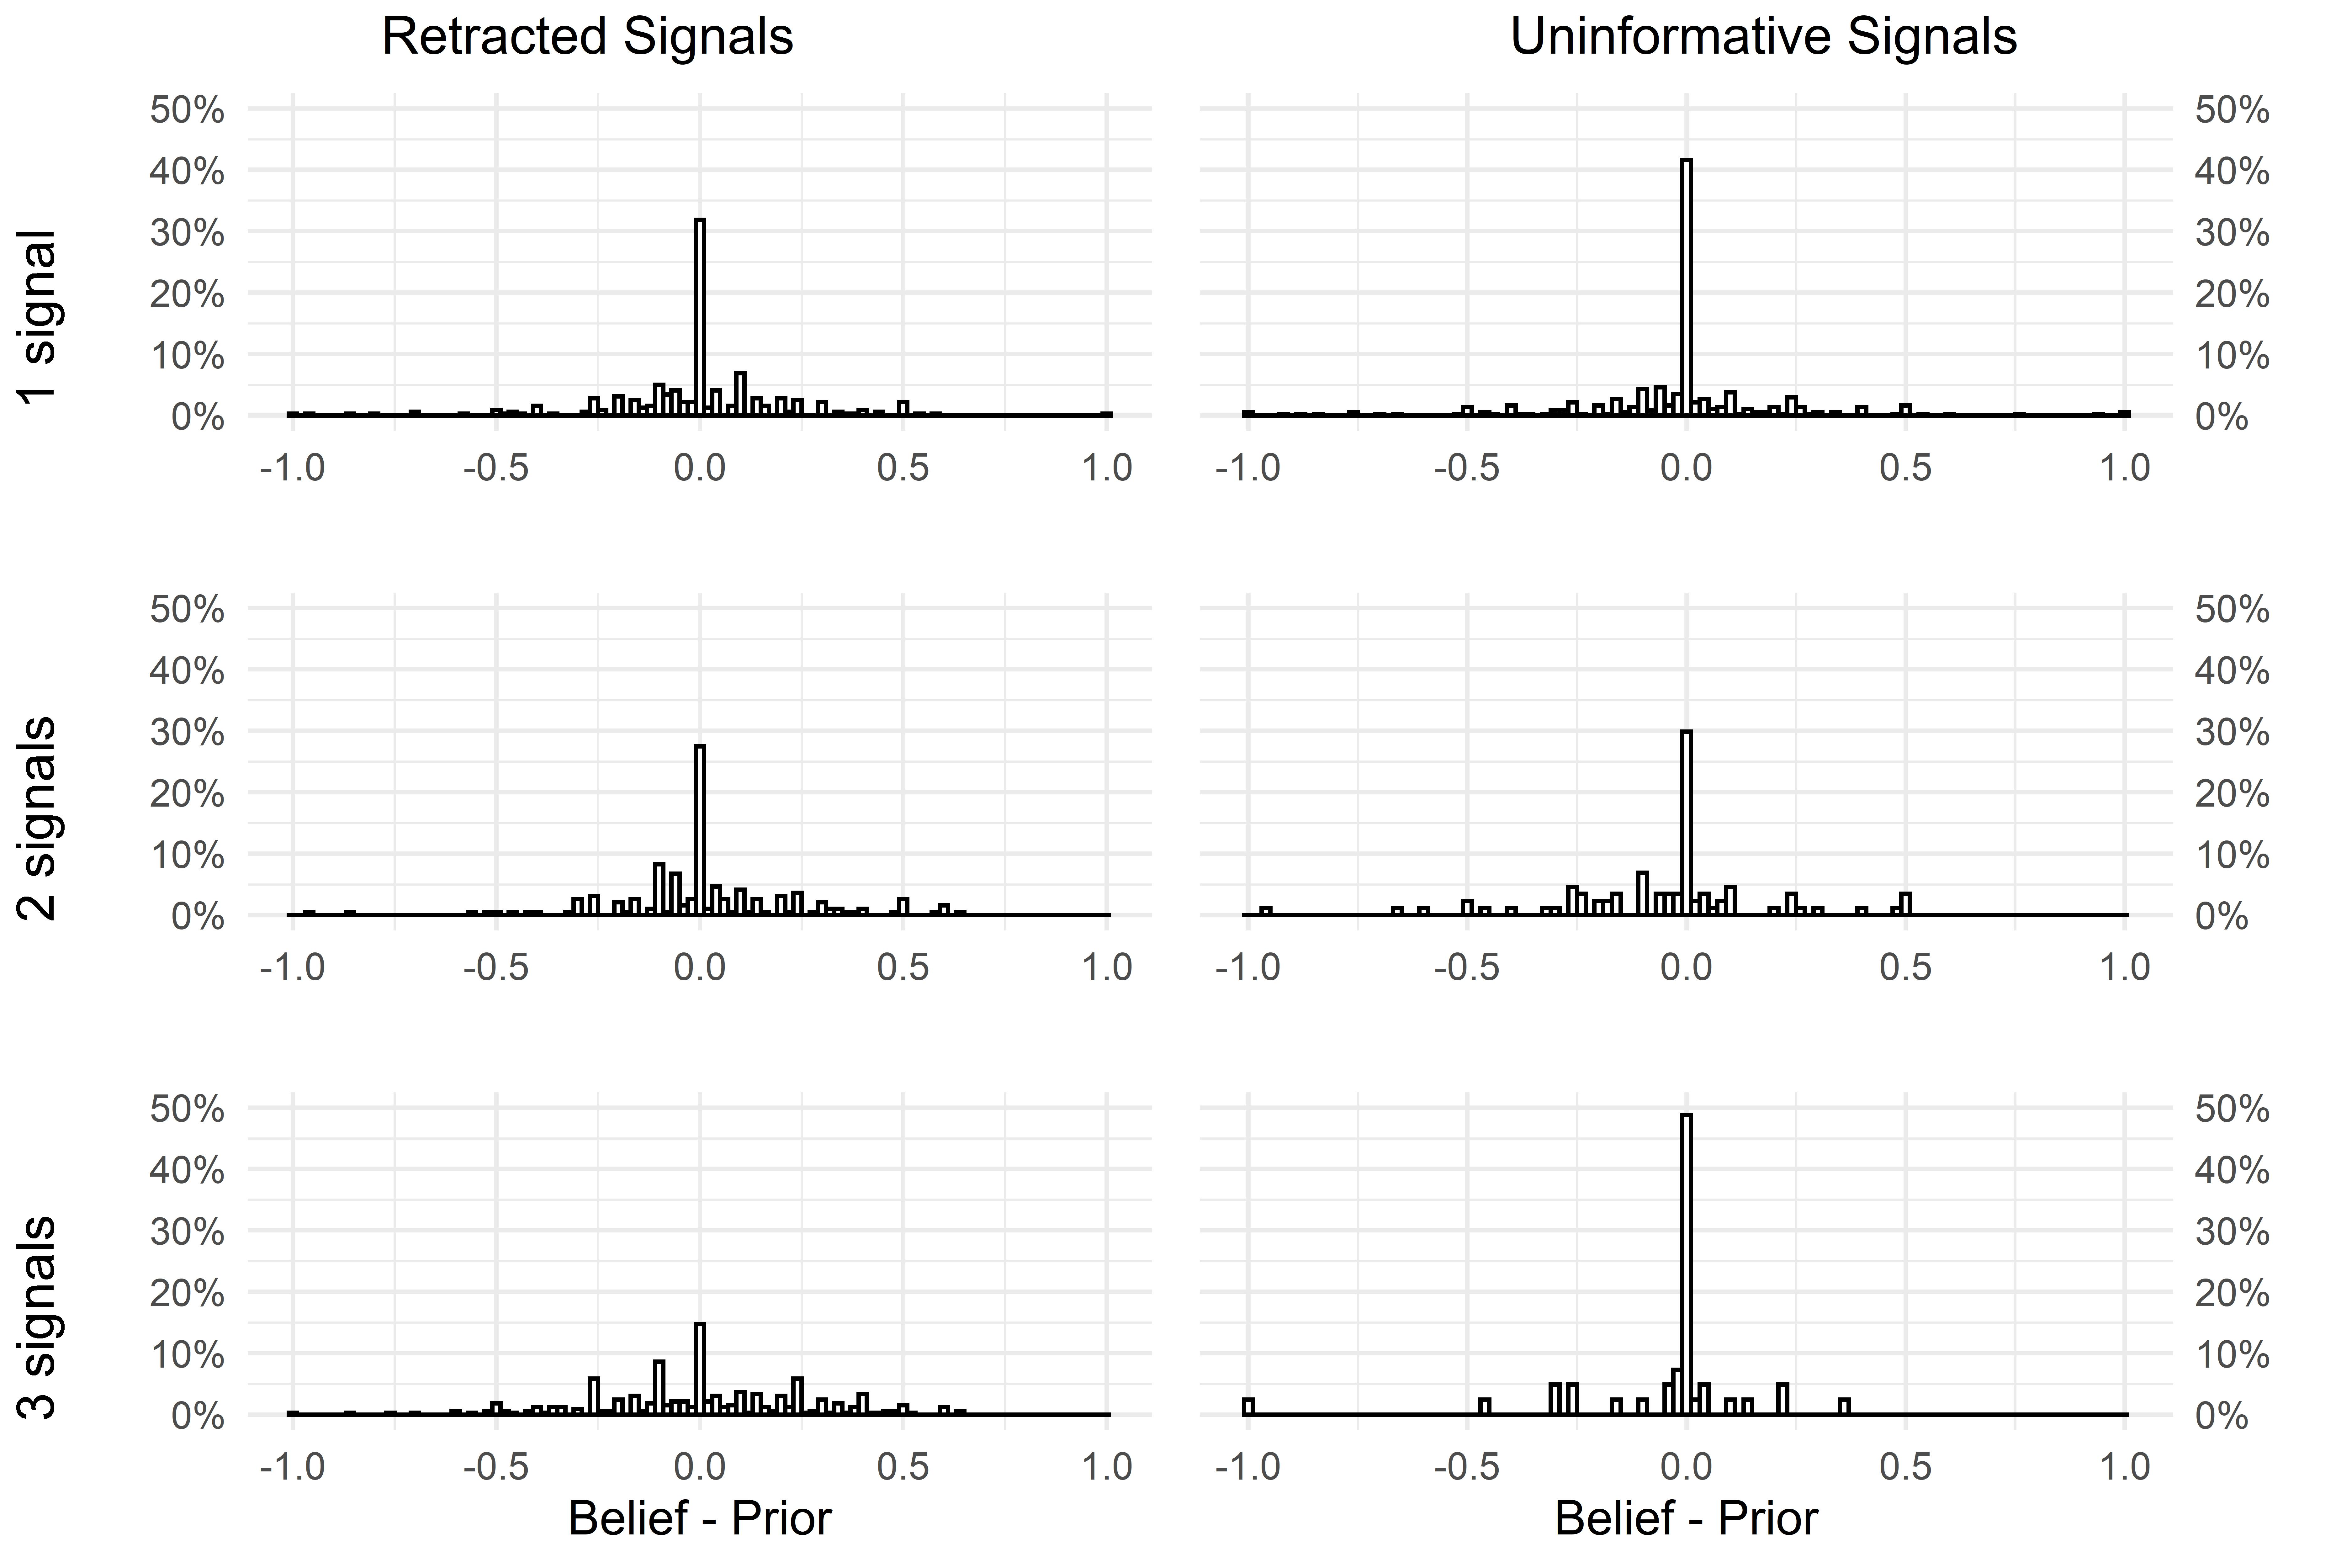
\includegraphics[width=12cm]{Fig/02_fig_variance_retract_uninf.jpg}
    \caption{Belief dispersion after multiple consecutive retracted signals vs uninformative signals. Histogram of belief difference to the prior, normalized by the number of subjects.}
    \label{fig:variance_retract_uninformative}
\end{figure}


\subsubsection{Informative Signals}
An informative signal in our design is a combination of a regular signal (i.e. the color of a ball) and the additional information that this ball is informative (i.e. it did indeed come from the randomly selected urn). For a rational subject, a confirmation of some initial signal should lead to the same belief as an informative signal for any given history of signals.

We find that, on average subjects appear to react stronger to an informative signal than a confirmed signal. Figure \ref{fig:informative_vs_confirmation} shows a clear comparison. On average, subjects reported a belief roughly 3 percentage points higher/lower following an informative red/blue signal, compared to the equivalent confirmed signal. This further exacerbates Result \ref{res:confirm} that subjects under-react to confirmations.

\begin{figure}[!htb]
    \centering
    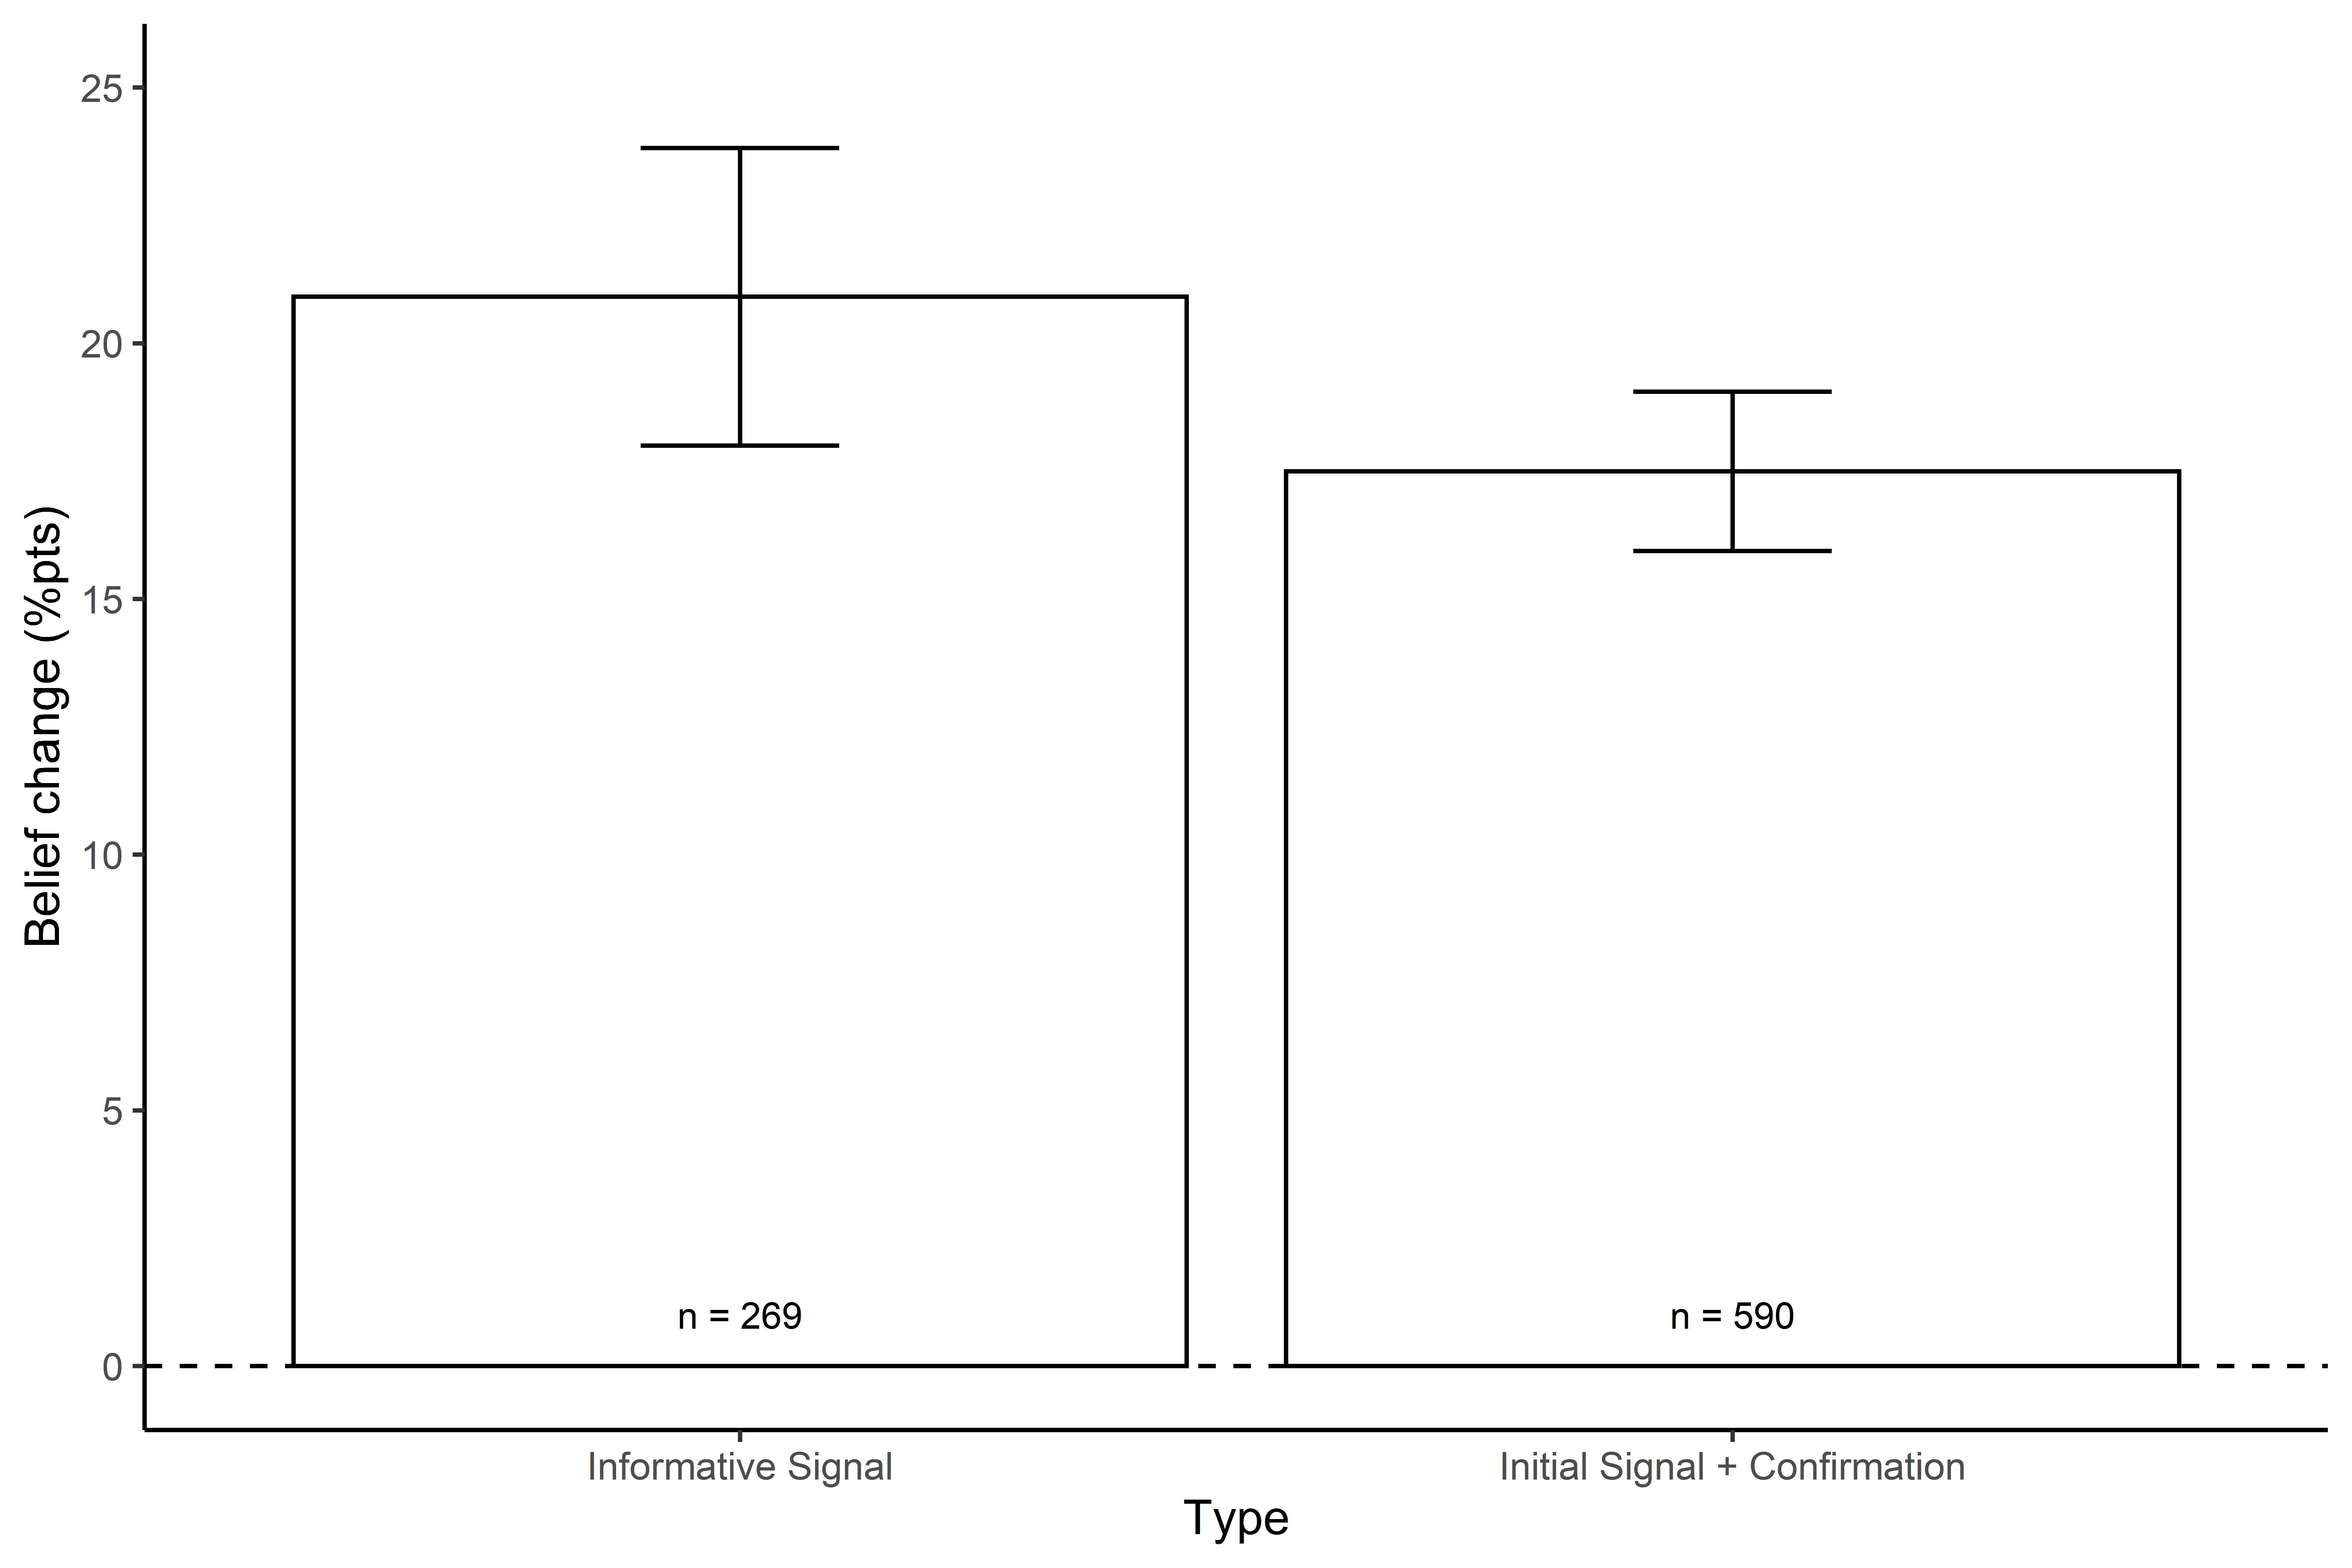
\includegraphics[width=10cm]{Fig/02_fig_confirm_vs_informative_change.jpg}
    \caption{Average belief change following an informative/confirmed signal, adjusted for the signal direction.}
    \label{fig:informative_vs_confirmation}
\end{figure}

As for uninformative signals, we can compare beliefs after confirmations to beliefs after informative signals for each exact history of previously observed signals. We define the aggregated history, $A(H_t)$, in the same as described before. Also, $I(H_t)$ denotes the sequence of informative signals, similar to before. Formally, we estimate the following regression:
\begin{equation}
    b_t(R|\mathbf{s_1},...,\mathbf{s_t})=\alpha + \beta \cdot F_{I(H_t)} + \gamma \cdot F_{A(H_t)} + \epsilon_t
\end{equation}
where $F_{I(H_t)}$ is a factor variable for all possible combinations of informative signals and $F_{A(H_t)}$ is a factor variable for all 'aggregated' histories, i.e.  histories with confirmed signals are coded the same as histories with informative signals. Any coefficient $\beta$ that is non-zero indicates differences between informative signals and confirmed signals. The results are reported in Table \ref{tab:confirm_vs_informative}. We find that while the coefficients are qualitatively in line with the prediction that people respond more to informative signals than confirmed signals, the majority of coefficients are not significantly different from zero. A effect of three percentage points as found above is not significant due to a relatively small number of histories that can be compared for informative/confirmed signals.


\subsection{Impact of Previous Information Checks}

The fourth and final research question we analyse is whether retractions, confirmations or ex-ante verifications in the past affect how people respond to uncertain information in the future. To answer this question we run two sets of regressions. The first set of regressions estimates inference from new information and base-rate use. It follows the method described above in equation \ref{eq-reg-inference}. We add several sets of explanatory variables regarding the number of past retractions and confirmations, if the color of the signal is the same or different to past retracted/confirmed ones, and the round in the experiment to rule out any potential time confound. All of those explanatory variables are interacted with the inference and base-rate use. The second set of regressions does not use log-likelihood ratios but absolute belief changes in response to a new ball draw (adjusted for the signal direction). Again we include the same explanatory variables regarding past retractions and confirmations, the ball color and the round number.

\begin{Result}
Previous ex-post checks have no clear effect on updating in the future.
\end{Result}

The regression results are reported in Tables \ref{tab:regular_verifications_llr} and \ref{tab:regular_verifications_belief_change}. In Table \ref{tab:regular_verifications_llr} it seems information checks of other colored balls in the past lowers inference in the future. However, this is not confirmed by the findings reported in Table BBB. Overall, while some coefficients appear to be significantly different from zero these findings are not supported by an intuitive explanation and also not supported by further analysis. Therefore, it seems that in general there is no clear affect of past information checks on future updating.


\section{Conclusion}
In this paper we set out to cleanly study how people process information about previous information through multiple closely related research questions. We introduce a novel modification of a well-studied framework by adding information uncertainty. Our framework allows us to unambiguously retract or confirm information after subjects see some uncertain information initially.

We have shown that the majority of subjects make mistakes when confronted with information about previous information, even in the relatively simpler case of retractions. Importantly, those mistakes are systematic and can be predicted by people's reaction to the initially uncertain information. With retracted information, only people that updated in a Bayesian way at first correctly returned to their initial prior belief. People that over-reacted to the uncertain information continued to be influenced by it after its retraction. Vice versa, people that under-reacted at first ended up with a belief lower than their initial prior belief. This implies that continued fake information, even if retracted immediately after it is seen, can lead to wildly dispersed belief. We find that, indeed, the variance in beliefs is substantially higher after multiple consecutive retracted pieces of information compared to equivalent information that is labeled as uninformative when people see it. 

We further find that in general subjects tended to be overly critical with confirmations of previously uncertain information. They inferred less from the confirmed signal than an equivalent informative signal. Finally, previous information checks in the form of retractions of confirmations did not seem to impact how subjects responded to new uncertain information, at least in our neutral setting.

Taken together, our findings have important implications for the way uncertain information is communicated in practice. Telling people information which is not verified ex-ante can lead to undesired effects after further information about the previous information is published. People might end up with substantially biased beliefs after a retraction or they may infer too little from a confirmation. Moreover, it is likely that the introduction of motivated reasoning and other context dependent features will amplify the bias in information processing we documented. Finally, it implies that the presence of continued misinformation is likely one driver for increasing belief dispersion, and in the extreme, belief polarization.

\newpage
\bibliography{BeliefUpdating}


\newpage
\appendix

\section{Tables and Figures}

\subsection{Overview}

% Table Correlation beliefs and bayesian

% Table created by stargazer v.5.2.2 by Marek Hlavac, Harvard University. E-mail: hlavac at fas.harvard.edu
% Date and time: Tue, Jan 24, 2023 - 10:08:03 AM
\begin{table}[!htbp] \centering 
  \caption{OLS Regression Output} 
  \label{tab:belief_bayesian} 
\begin{tabular}{@{\extracolsep{5pt}}lc} 
\\[-1.8ex]\hline 
\hline \\[-1.8ex] 
 & \multicolumn{1}{c}{\textit{Dependent variable:}} \\ 
\cline{2-2} 
\\[-1.8ex] & Reported Belief \\ 
\hline \\[-1.8ex] 
 Constant & 0.134$^{***}$ \\ 
  & (0.008) \\ 
  Bayesian Posterior & 0.718$^{***}$ \\ 
  & (0.016) \\ 
 \hline \\[-1.8ex] 
Observations & 8,397 \\ 
Adjusted R$^{2}$ & 0.495 \\ 
\hline 
\hline \\[-1.8ex] 
\textit{Note:}  & \multicolumn{1}{r}{$^{*}$p$<$0.1; $^{**}$p$<$0.05; $^{***}$p$<$0.01} \\ 
 & \multicolumn{1}{r}{SEs clustered by subject.} \\ 
\end{tabular} 
\end{table} 

\noindent\textit{Notes:} Bayesian posteriors are based on sequential updating, i.e. the subject's previous posterior belief serves as his prior when shown new information.

% Table on regular updating - Estimating inference and base-rate use

% Table created by stargazer v.5.2.2 by Marek Hlavac, Harvard University. E-mail: hlavac at fas.harvard.edu
% Date and time: Tue, Jan 17, 2023 - 1:02:31 PM
\begin{table}[!htbp] \centering 
  \caption{Updating with Regular Signals} 
  \label{tab:regular_updating} 
\begin{tabular}{@{\extracolsep{5pt}}lccc} 
\\[-1.8ex]\hline 
\hline \\[-1.8ex] 
 & \multicolumn{3}{c}{\textit{Dependent variable:}} \\ 
\cline{2-4} 
\\[-1.8ex] & \multicolumn{3}{c}{Observed Log-Posterior-Ratio} \\ 
\\[-1.8ex] & \textit{OLS} & \multicolumn{2}{c}{\textit{linear}} \\ 
 & \textit{} & \multicolumn{2}{c}{\textit{mixed-effects}} \\ 
\\[-1.8ex] & (1) & (2) & (3)\\ 
\hline \\[-1.8ex] 
 Constant & $-$0.041$^{*}$ & $-$0.029 & $-$0.031 \\ 
  & (0.022) & (0.020) & (0.020) \\ 
  Signal & 1.530$^{***}$ & 1.538$^{***}$ & 1.400$^{***}$ \\ 
  & (0.051) & (0.052) & (0.067) \\ 
  Prior & 0.697$^{***}$ & 0.721$^{***}$ & 0.690$^{***}$ \\ 
  & (0.027) & (0.019) & (0.021) \\ 
  Signal Confirms Prior &  &  & 0.354$^{***}$ \\ 
  &  &  & (0.107) \\ 
 \hline \\[-1.8ex] 
Observations & 6,777 & 6,777 & 6,777 \\ 
Adjusted R$^{2}$ & 0.480 &  &  \\ 
Log Likelihood &  & $-$12,811.120 & $-$12,807.140 \\ 
Akaike Inf. Crit. &  & 25,642.230 & 25,636.280 \\ 
Bayesian Inf. Crit. &  & 25,710.450 & 25,711.310 \\ 
\hline 
\hline \\[-1.8ex] 
\textit{Note:}  & \multicolumn{3}{r}{$^{*}$p$<$0.1; $^{**}$p$<$0.05; $^{***}$p$<$0.01} \\ 
 & \multicolumn{3}{r}{SEs clustered by subject.} \\ 
\end{tabular} 
\end{table} 

\break

% Type distribution inference and base-rate use
\begin{figure}[!ht]
    \centering
    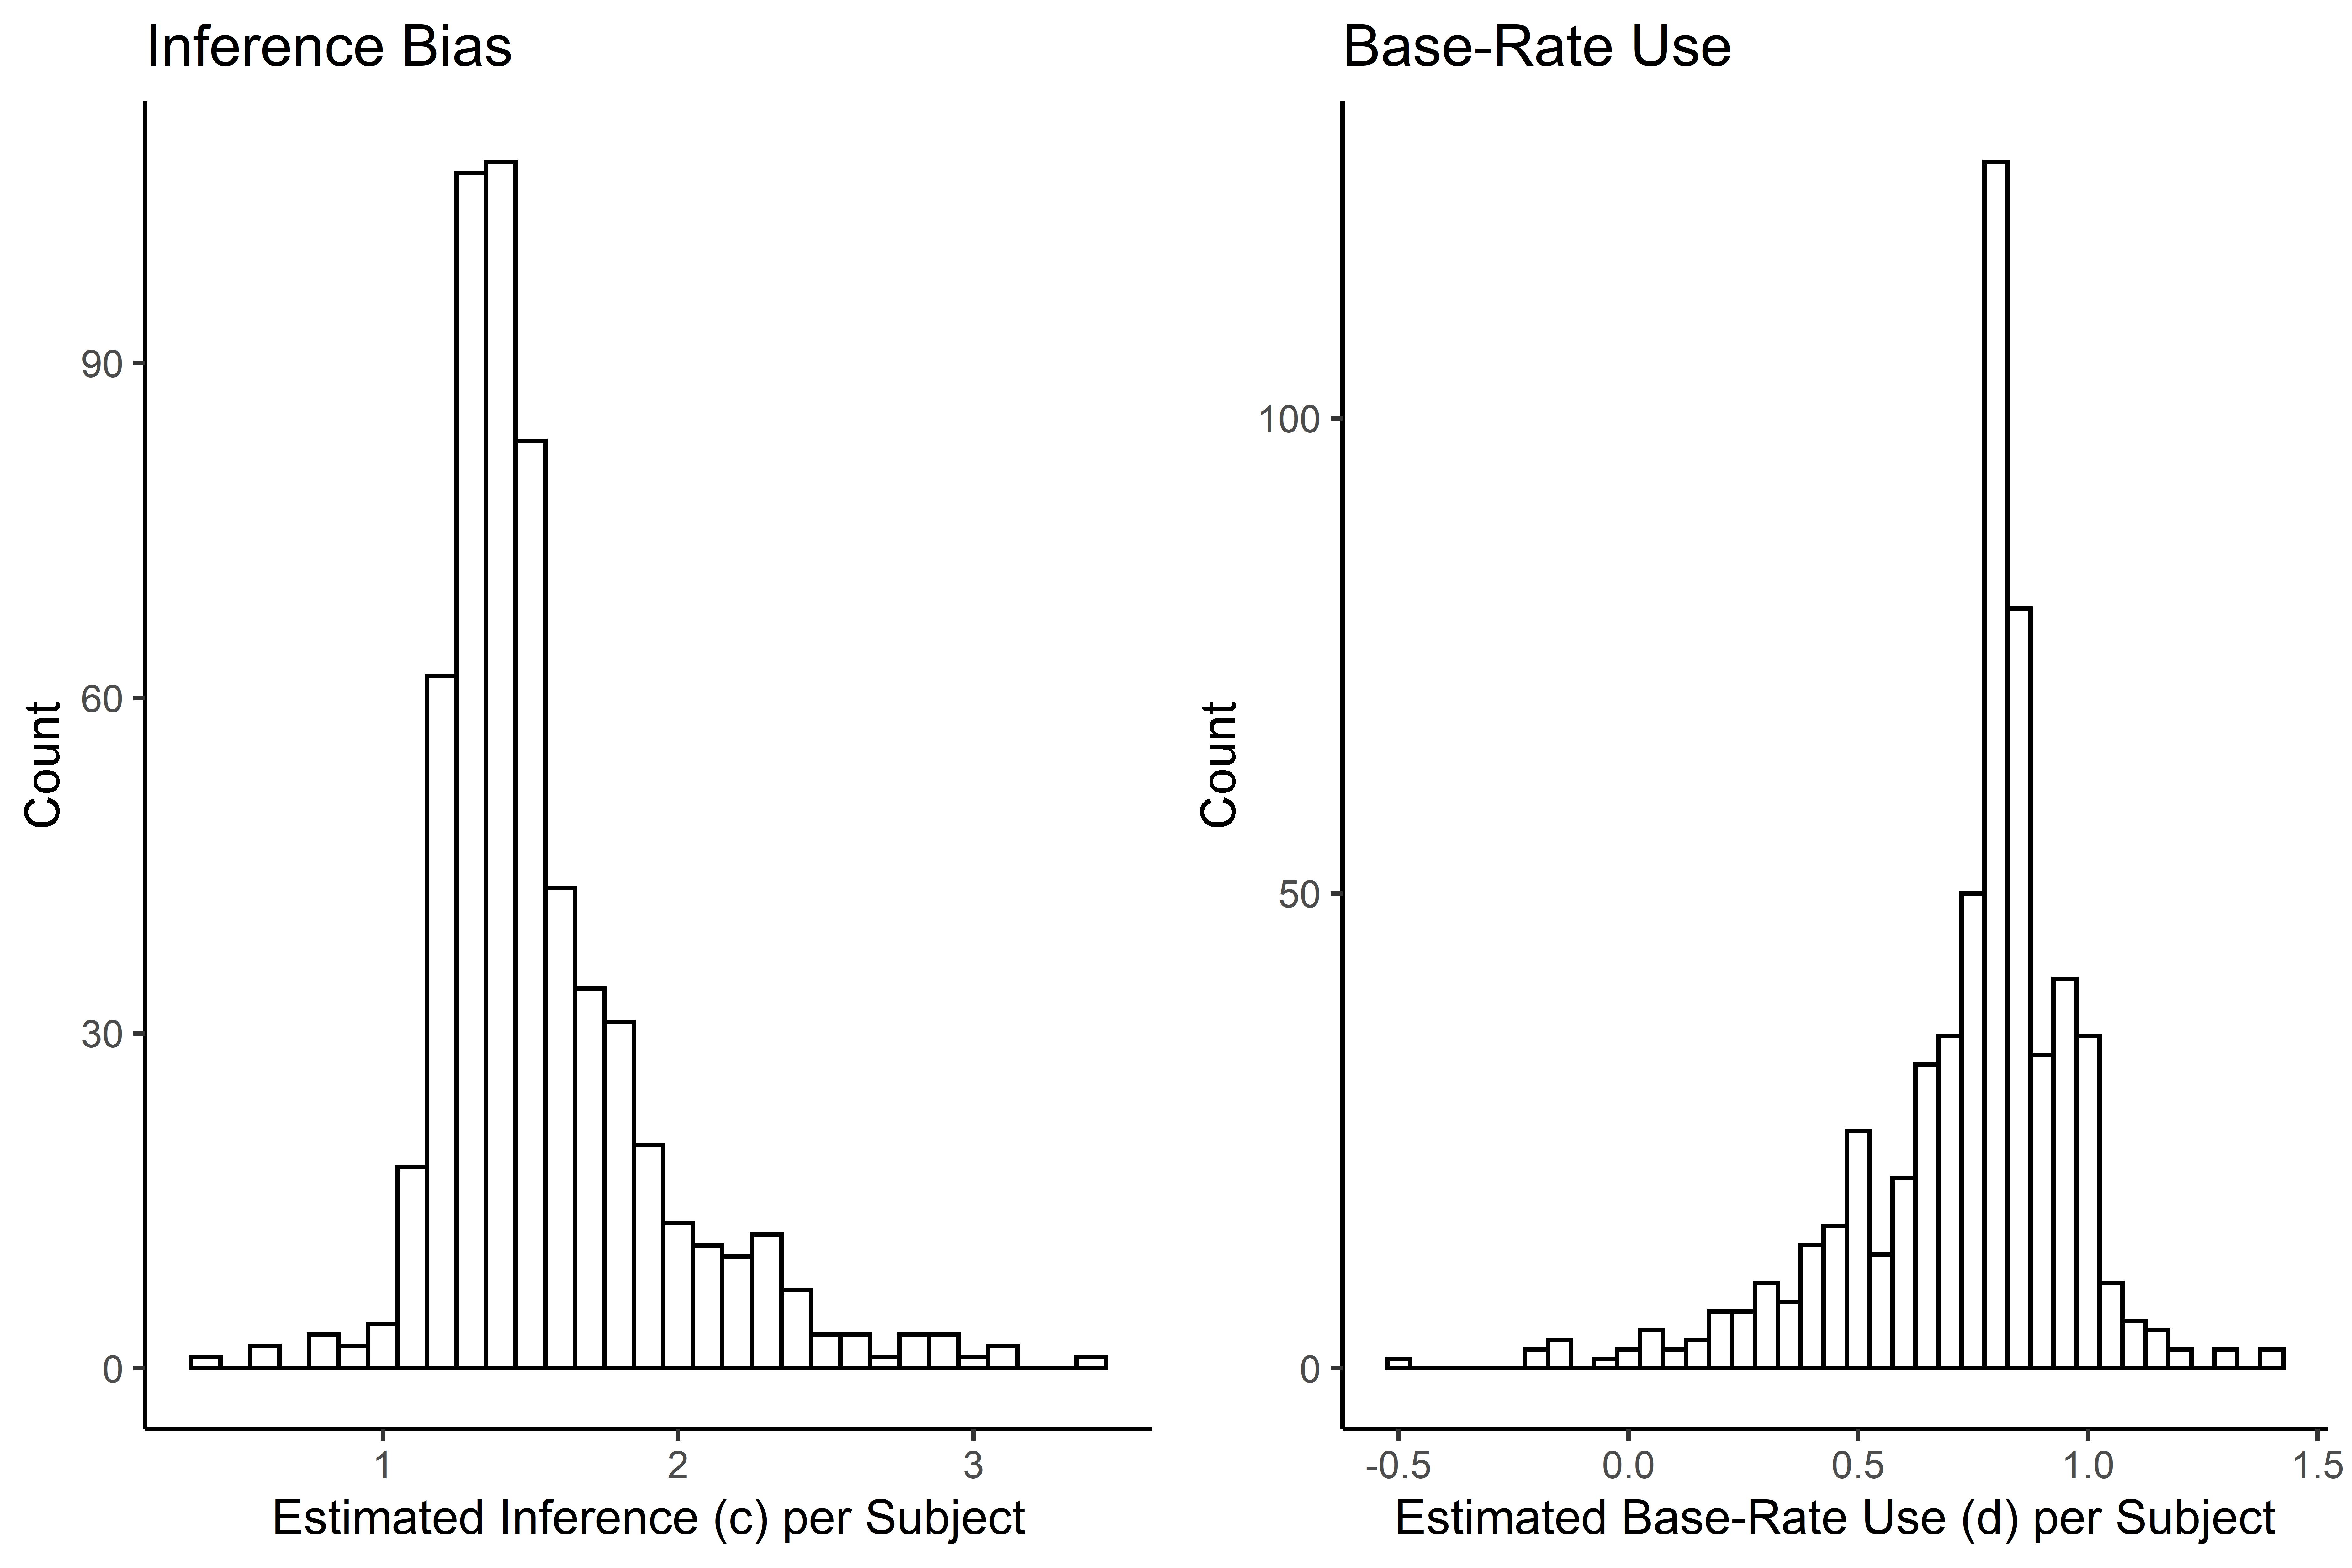
\includegraphics[width=12cm]{Fig/04_fig_regular_updating_type_dist.jpg}
    \caption{Distribution of average inference and base-rate use per subject. Note that a parameter of 1 for both would be equivalent with Bayesian updating.}
    \label{fig:regular_inf_baserate_type_dist}
\end{figure}

\vspace{1cm}

% Type distribution average difference bayesian
\begin{figure}[!ht]
    \centering
    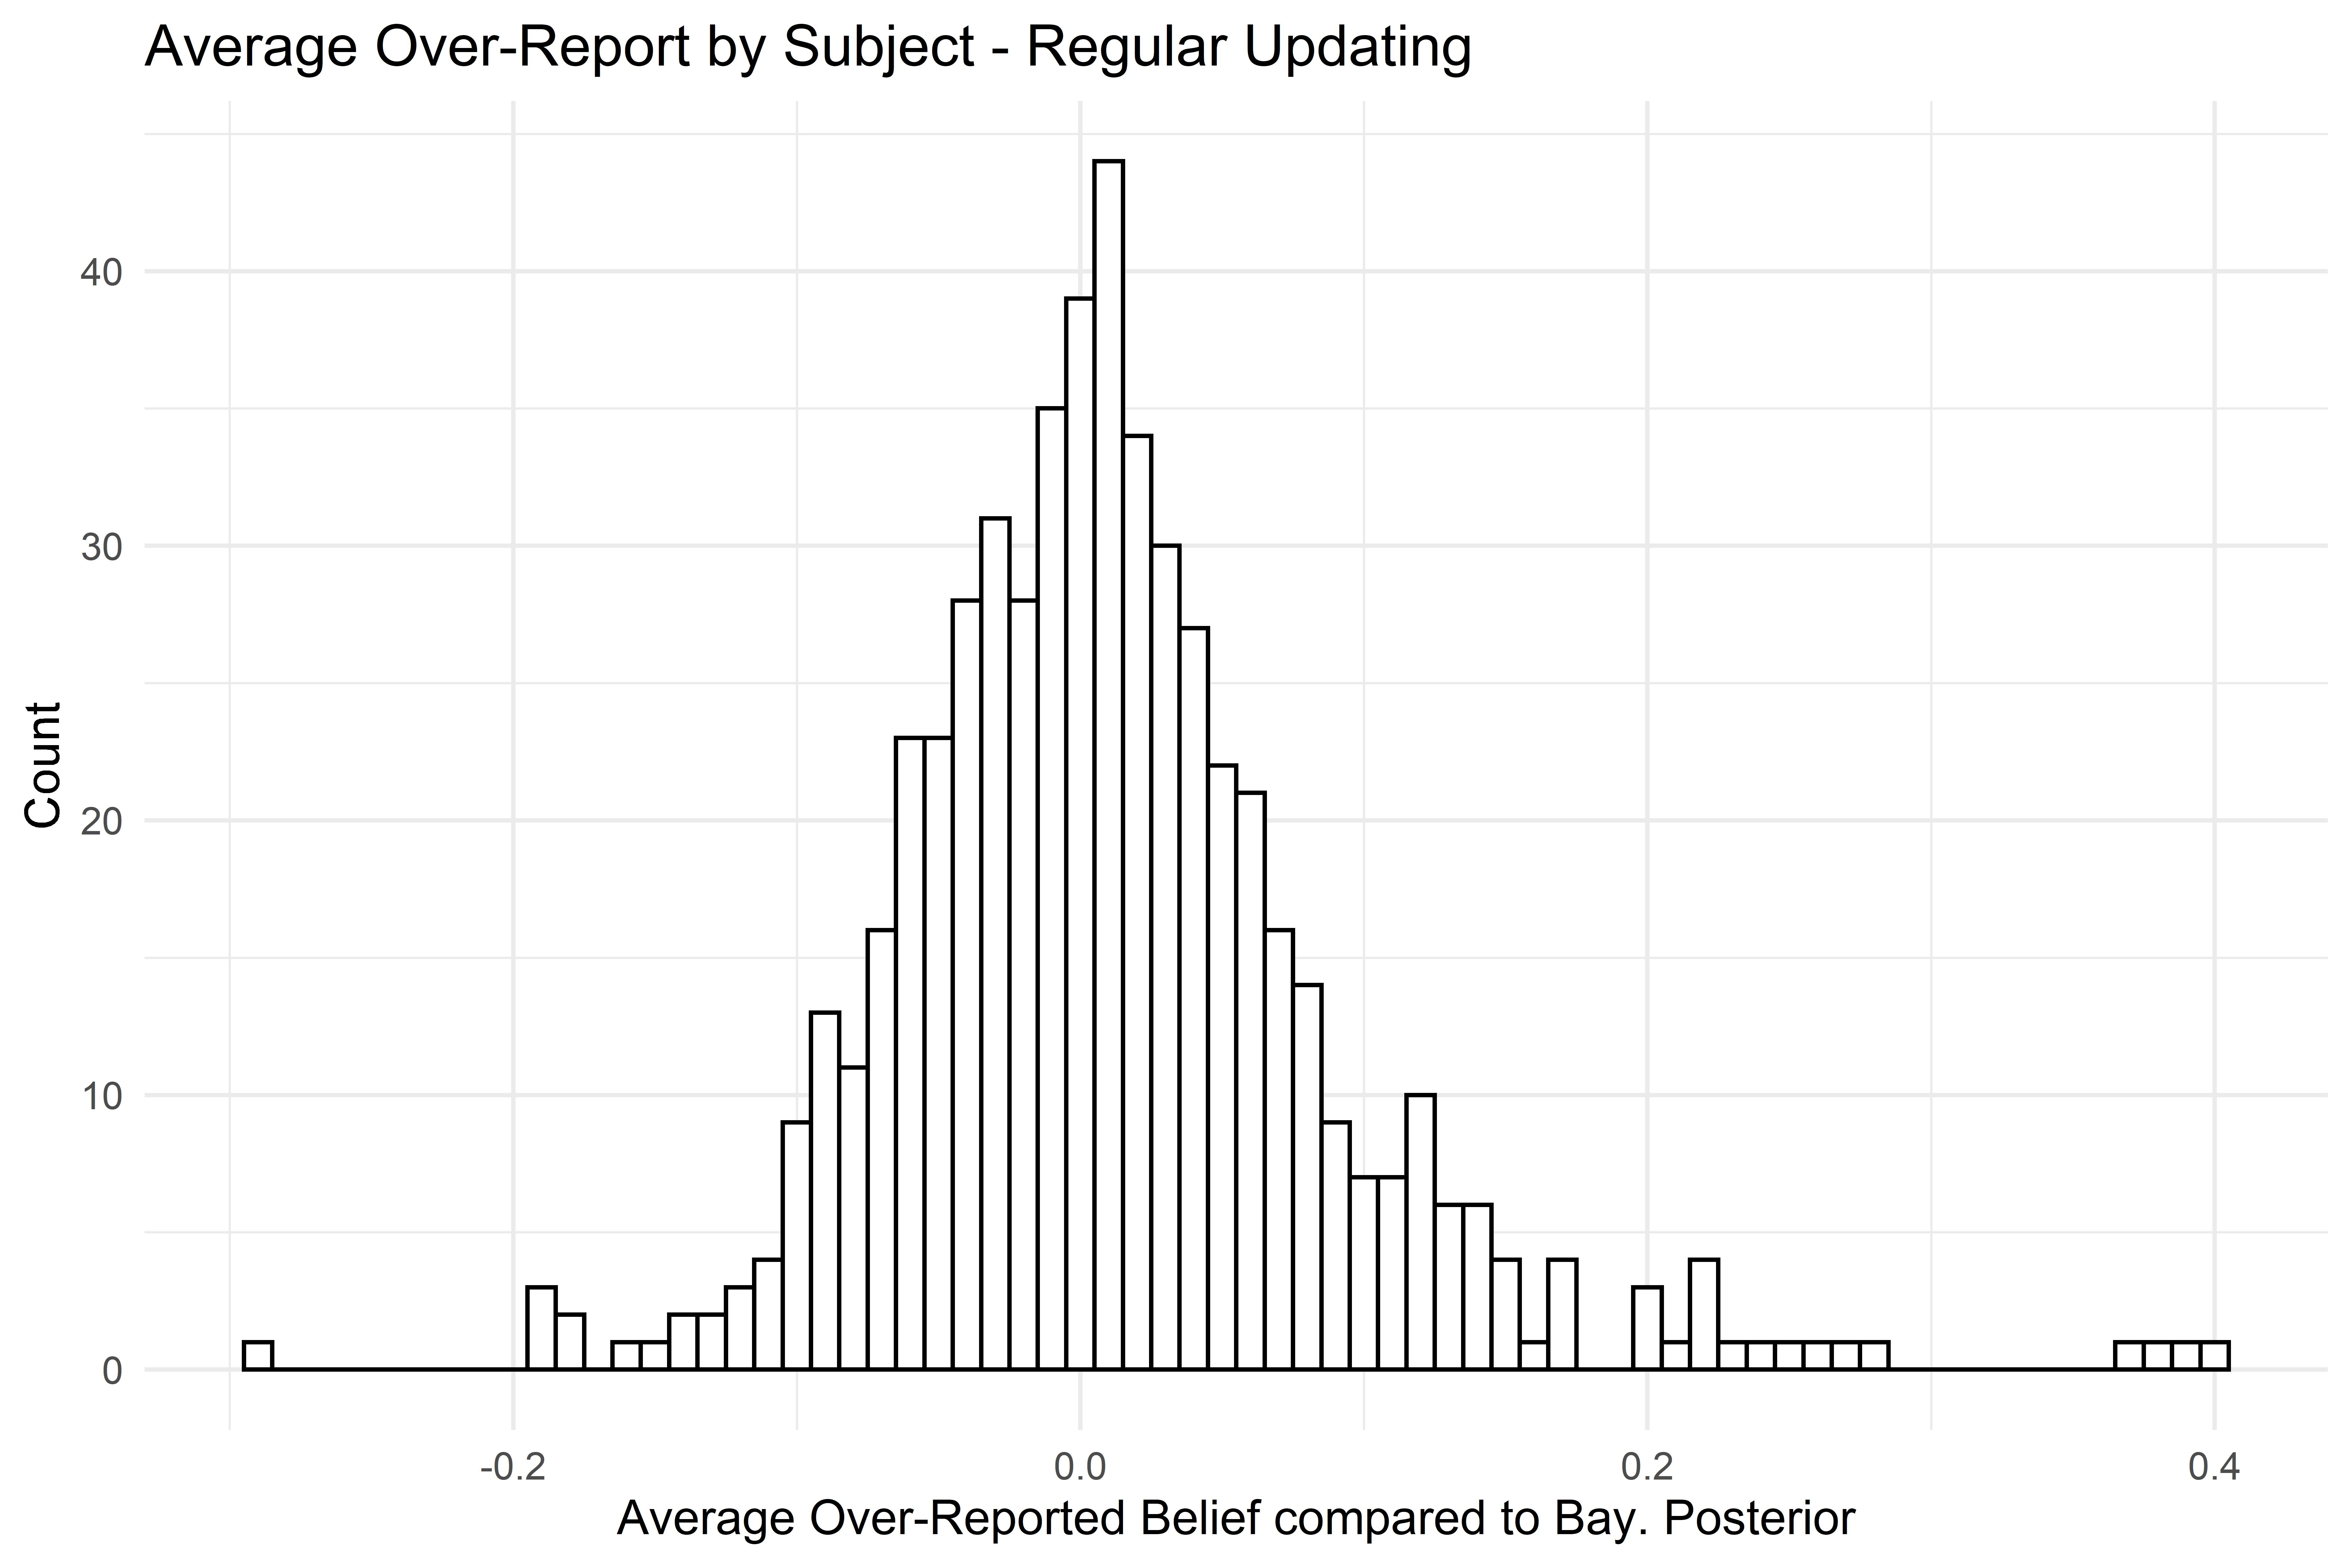
\includegraphics[width=12cm]{Fig/02_fig_belief_distance_type_avg.jpg}
    \caption{Average bias per subject. A value of zero is equivalent to Bayesian updating on average.}
    \label{fig:regular_belief_diff_type}
\end{figure}

% Table for treatment differences with regular updating

% Table created by stargazer v.5.2.2 by Marek Hlavac, Harvard University. E-mail: hlavac at fas.harvard.edu
% Date and time: Mon, Jan 30, 2023 - 3:49:30 PM
\begin{table}[!htbp] \centering \small
  \caption{Updating with Regular Signals - Effect of Varying Information Display} 
  \label{tab:regular_treat} 
\begin{tabular}{@{\extracolsep{5pt}}lc} 
\\[-1.8ex]\hline 
\hline \\[-1.8ex] 
 & \multicolumn{1}{c}{\textit{Dependent variable:}} \\ 
\cline{2-2} 
\\[-1.8ex] & Observed Log-Posterior-Ratio \\ 
 & Benchmark \\ 
\hline \\[-1.8ex] 
 Constant & $-$0.035 \\ 
  & (0.035) \\ 
  Treat: No prev. belief & $-$0.047 \\ 
  & (0.055) \\ 
  Treat: No history & 0.036 \\ 
  & (0.055) \\ 
  Signal & 1.465$^{***}$ \\ 
  & (0.088) \\ 
  Signal * Treat: No prev. belief & 0.084 \\ 
  & (0.138) \\ 
  Signal * Treat: No history & $-$0.049 \\ 
  & (0.136) \\ 
  Prior & 0.750$^{***}$ \\ 
  & (0.040) \\ 
  Prior * Treat: No prev. belief & $-$0.053 \\ 
  & (0.060) \\ 
  Prior * Treat: No history & $-$0.174$^{**}$ \\ 
  & (0.082) \\ 
 \hline \\[-1.8ex] 
Observations & 6,093 \\ 
Adjusted R$^{2}$ & 0.473 \\ 
\hline 
\hline \\[-1.8ex] 
\textit{Note:}  & \multicolumn{1}{r}{$^{*}$p$<$0.1; $^{**}$p$<$0.05; $^{***}$p$<$0.01} \\ 
 & \multicolumn{1}{r}{SEs clustered by subject.} \\ 
\end{tabular} 
\end{table} 



\newpage
\subsection{Retractions}

% Figure for belief change initial vs retraction
\begin{figure}[!htb]
    \centering
    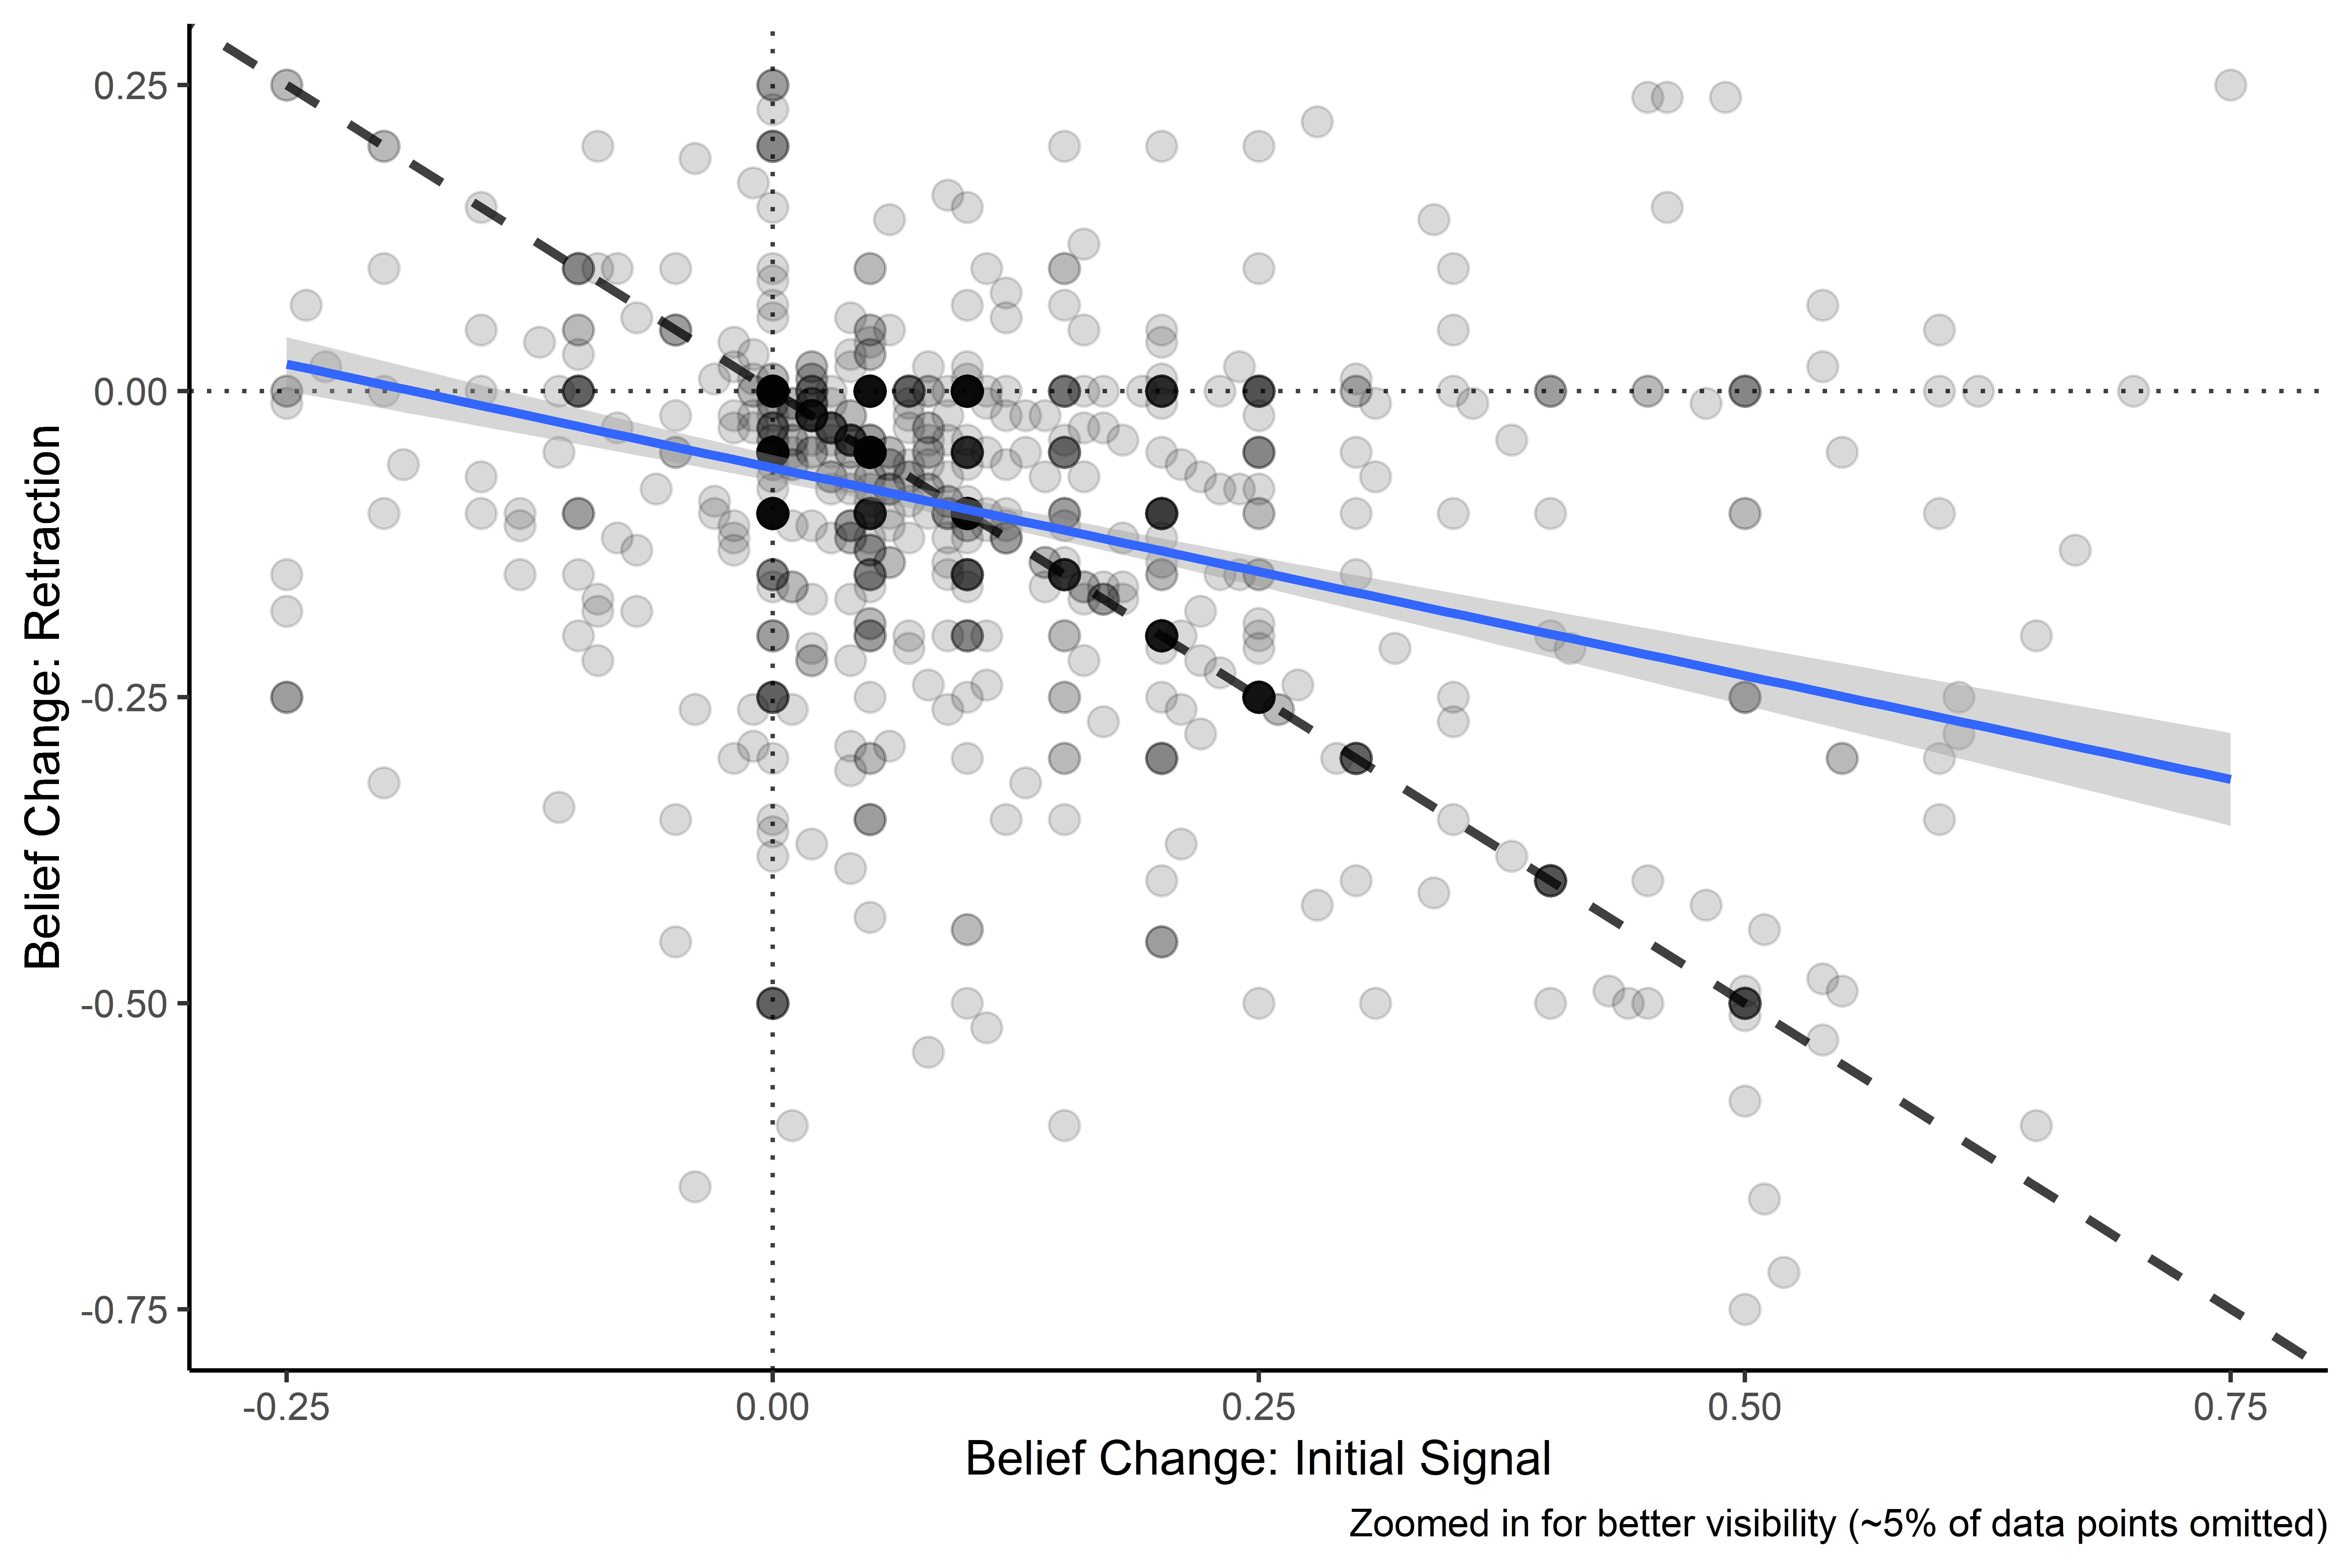
\includegraphics[width = 12cm]{Fig/02_fig_retract_change_lm.jpg}
    \caption{Scatter plot of belief change after the retraction by initial belief change, controlling for the signal direction. A rational response to the retraction would lead to an observation displayed on the diagonal. All observations north-east of the diagonal are from subjects that under-reacted to the retraction and observations south-west of the diagonal are from subjects that over-reacted.}
    \label{fig:retract_change}
\end{figure}

% Table on impact of retractions 

% Table created by stargazer v.5.2.2 by Marek Hlavac, Harvard University. E-mail: hlavac at fas.harvard.edu
% Date and time: Thu, Dec 01, 2022 - 12:59:44 PM
\begin{table}[!htbp] \centering 
  \caption{Impact of Retractions on Beliefs} 
  \label{tab:retractions_main} 
\begin{tabular}{@{\extracolsep{5pt}}lc} 
\\[-1.8ex]\hline 
\hline \\[-1.8ex] 
 & \multicolumn{1}{c}{\textit{Dependent variable:}} \\ 
\cline{2-2} 
\\[-1.8ex] & Belief minus Bayesian Posterior \\ 
\hline \\[-1.8ex] 
 Constant & $-$0.004 \\ 
  & (0.006) \\ 
  Belief minus Bayesian Posterior Previously & 0.614$^{***}$ \\ 
  & (0.052) \\ 
 \hline \\[-1.8ex] 
Observations & 985 \\ 
Adjusted R$^{2}$ & 0.309 \\ 
\hline 
\hline \\[-1.8ex] 
\textit{Note:}  & \multicolumn{1}{r}{$^{*}$p$<$0.1; $^{**}$p$<$0.05; $^{***}$p$<$0.01} \\ 
 & \multicolumn{1}{r}{SEs clustered by subject.} \\ 
\end{tabular} 
\end{table} 

\vspace{2cm}

% Figure on impact of retractions
\begin{figure}[!ht]
    \centering
    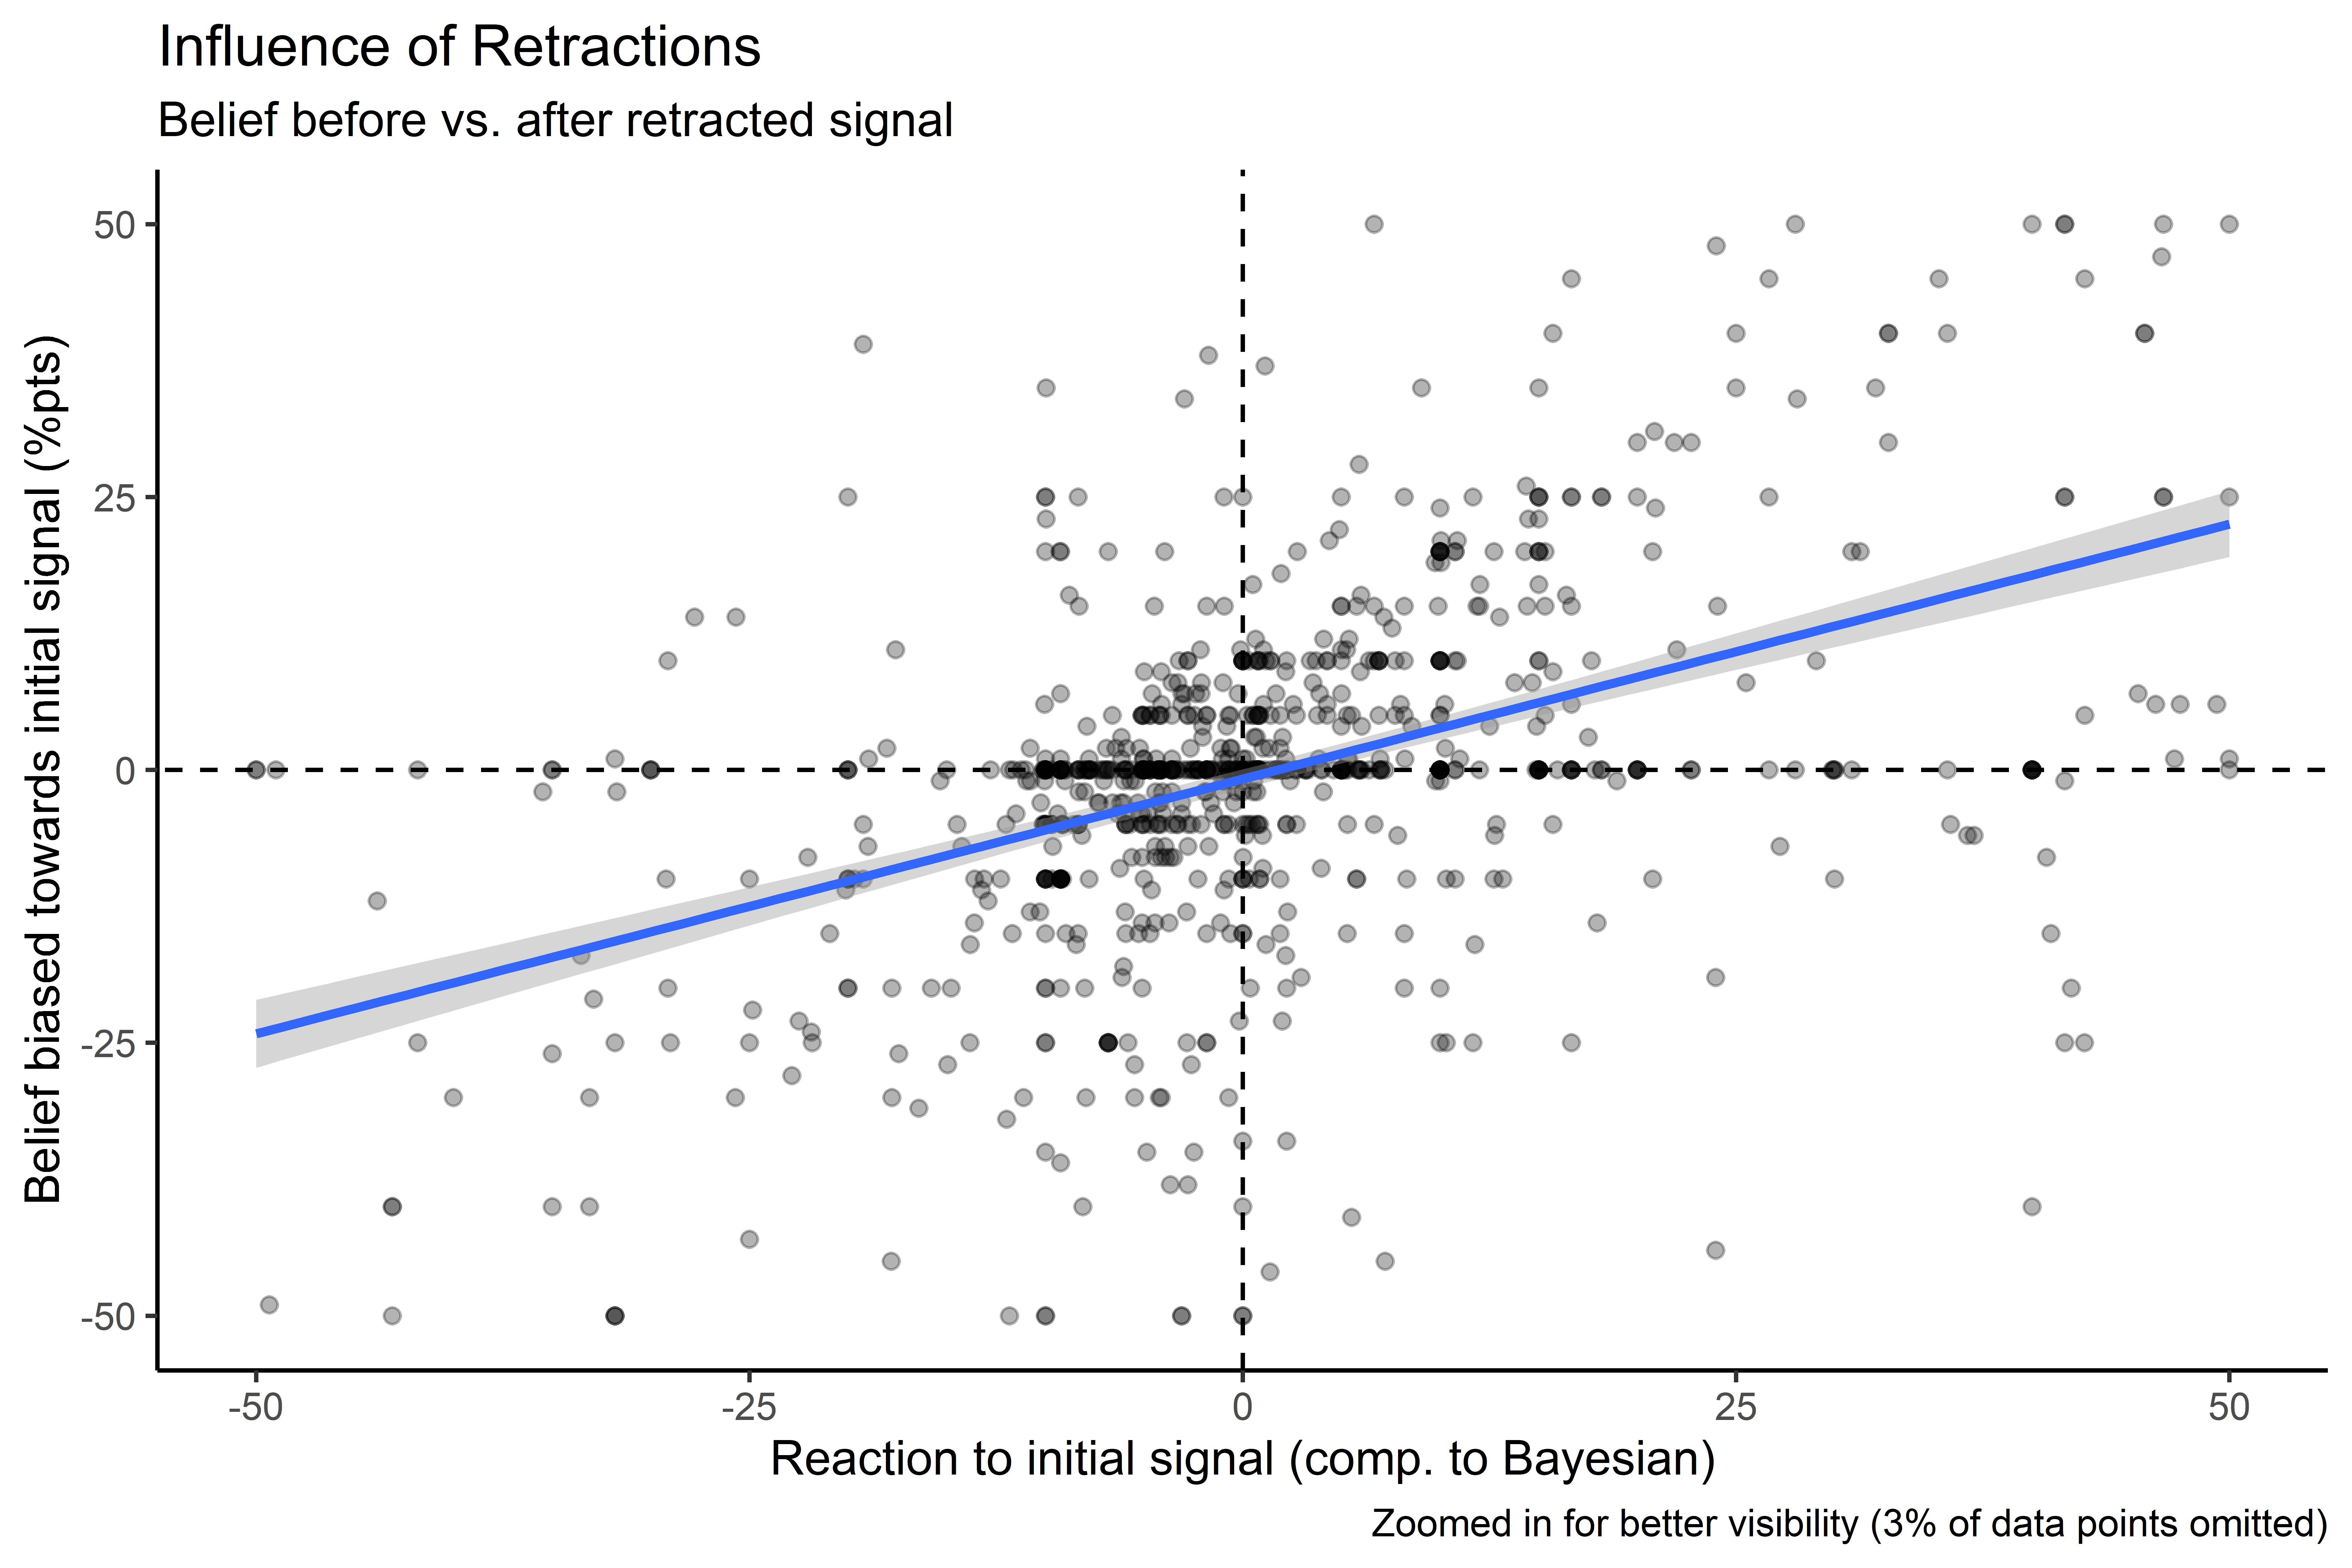
\includegraphics[width=12cm]{Fig/02_fig_retract_diff_cont_noout.jpg}
    \caption{Overview of all individual belief reports following a retraction. All observations along the horizontal line indicate a rational response to the retraction (irrespective of the initial belief update). All observations along the vertical line indicate a rational response to the initial uncertain signal.}
    \label{fig:belief_diff_retract}
\end{figure}

% Regression retractions - compressed histories

% Table created by stargazer v.5.2.2 by Marek Hlavac, Harvard University. E-mail: hlavac at fas.harvard.edu
% Date and time: Thu, Dec 01, 2022 - 12:56:10 PM
\begin{table}[!htbp] \centering \footnotesize
  \caption{Impact of Retractions} 
  \label{tab:retraction_compressed_histories} 
\begin{tabular}{@{\extracolsep{5pt}}lcc} 
\\[-1.8ex]\hline 
\hline \\[-1.8ex] 
 & \multicolumn{2}{c}{\textit{Dependent variable:}} \\ 
\cline{2-3} 
\\[-1.8ex] & \multicolumn{2}{c}{Reported Belief} \\ 
\\[-1.8ex] & (1) & (2)\\ 
\hline \\[-1.8ex] 
 Retraction & $-$0.018$^{**}$ & $-$0.014 \\ 
  & (0.009) & (0.009) \\ 
  Retraction History: R & 0.009 & 0.004 \\ 
  & (0.010) & (0.011) \\ 
  Retraction History: B & $-$0.011 & $-$0.017 \\ 
  & (0.009) & (0.011) \\ 
  Retraction History: RR & 0.018 & 0.005 \\ 
  & (0.014) & (0.016) \\ 
  Retraction History: BB & $-$0.028$^{**}$ & $-$0.041$^{**}$ \\ 
  & (0.013) & (0.016) \\ 
  Retraction History: RB & 0.015 & 0.002 \\ 
  & (0.014) & (0.016) \\ 
  Retraction History: BR & $-$0.003 & $-$0.016 \\ 
  & (0.015) & (0.017) \\ 
  Retraction History: RRR & 0.050$^{**}$ & 0.031 \\ 
  & (0.020) & (0.024) \\ 
  Retraction History: BBB & $-$0.027 & $-$0.048$^{*}$ \\ 
  & (0.024) & (0.027) \\ 
  Retraction History: RRB & 0.062 & 0.044 \\ 
  & (0.040) & (0.042) \\ 
  Retraction History: BBR & 0.041$^{*}$ & 0.020 \\ 
  & (0.024) & (0.028) \\ 
  Retraction History: RBB & 0.024 & 0.005 \\ 
  & (0.024) & (0.027) \\ 
  Retraction History: BRR & 0.070$^{**}$ & 0.050 \\ 
  & (0.028) & (0.031) \\ 
  Retraction History: RBR & 0.012 & $-$0.008 \\ 
  & (0.028) & (0.031) \\ 
  Retraction History: BRB & 0.051$^{*}$ & 0.031 \\ 
  & (0.030) & (0.033) \\ 
 \hline \\[-1.8ex] 
Compressed History FEs? & Yes & Yes \\ 
Round FEs? & No & Yes \\ 
Observations & 6,480 & 6,480 \\ 
Adjusted R$^{2}$ & 0.505 & 0.505 \\ 
\hline 
\hline \\[-1.8ex] 
\textit{Note:}  & \multicolumn{2}{r}{$^{*}$p$<$0.1; $^{**}$p$<$0.05; $^{***}$p$<$0.01} \\ 
\end{tabular} 
\end{table} 


% Impact of retractions - inference and base-rate use

% Table created by stargazer v.5.2.2 by Marek Hlavac, Harvard University. E-mail: hlavac at fas.harvard.edu
% Date and time: Thu, Dec 01, 2022 - 1:14:37 PM
\begin{table}[!htbp] \centering 
  \caption{Updating with Retraction Signals} 
  \label{tab:retractions_inference} 
\begin{tabular}{@{\extracolsep{5pt}}lcccc} 
\\[-1.8ex]\hline 
\hline \\[-1.8ex] 
 & \multicolumn{4}{c}{\textit{Dependent variable:}} \\ 
\cline{2-5} 
\\[-1.8ex] & \multicolumn{4}{c}{Observed Log-Posterior-Ratio} 
\\ & All Retractions & Prev. Correct  & Prev. under-infered  & Prev. over-infered 
\\ & & (+- 1\%pt) & ($<$1\%pt) & ($>$1\%pt) \\
\\[-1.8ex] & (1) & (2) & (3) & (4)\\ 
\hline \\[-1.8ex] 
 Constant & $-$0.107$^{*}$ & $-$0.199 & 0.001 & $-$0.056 \\ 
  & (0.057) & (0.140) & (0.046) & (0.103) \\ 
  Retraction & 0.327$^{***}$ & 1.228$^{***}$ & 1.415$^{***}$ & 0.293$^{***}$ \\ 
  & (0.107) & (0.339) & (0.226) & (0.055) \\ 
  Prior & 0.793$^{***}$ & 0.788$^{***}$ & 0.998$^{***}$ & 0.786$^{***}$ \\ 
  & (0.065) & (0.045) & (0.056) & (0.063) \\ 
 \hline \\[-1.8ex] 
Observations & 985 & 166 & 190 & 377 \\ 
Adjusted R$^{2}$ & 0.425 & 0.653 & 0.624 & 0.318 \\ 
\hline 
\hline \\[-1.8ex] 
\textit{Note:}  & \multicolumn{4}{r}{$^{*}$p$<$0.1; $^{**}$p$<$0.05; $^{***}$p$<$0.01} \\ 
\end{tabular} 
\end{table} 


% Types - robustness

% Table created by stargazer v.5.2.2 by Marek Hlavac, Harvard University. E-mail: hlavac at fas.harvard.edu
% Date and time: Tue, Jan 10, 2023 - 2:14:13 PM
\begin{table}[!htbp] \centering 
  \caption{Different categorizations of types} 
  \label{tab:retractions_types} 
\begin{tabular}{@{\extracolsep{5pt}}lcccc} 
\\[-1.8ex]\hline 
\hline \\[-1.8ex] 
 & \multicolumn{4}{c}{\textit{Dependent variable:}} \\ 
\cline{2-5} 
\\[-1.8ex] & \multicolumn{4}{c}{Belief biased towards initial signal} \\ 
\\[-1.8ex] & (1) & (2) & (3) & (4)\\ 
\hline \\[-1.8ex] 
 Constant & 0.005 & 0.038$^{***}$ & $-$0.003 & 0.166 \\ 
  & (0.005) & (0.012) & (0.016) & (0.104) \\ 
  Initial belief over-report & 0.736$^{***}$ & 0.673$^{***}$ & 0.638$^{***}$ & 0.717$^{***}$ \\ 
  & (0.064) & (0.057) & (0.054) & (0.039) \\ 
  Average belief over-report & $-$0.552$^{***}$ &  &  &  \\ 
  & (0.118) &  &  &  \\ 
  Average inference (c-1) &  & $-$0.107$^{***}$ &  &  \\ 
  &  & (0.030) &  &  \\ 
  Average base-rate use (d-1) &  & $-$0.056 &  &  \\ 
  &  & (0.042) &  &  \\ 
  Type: Not categorized &  &  & $-$0.002 &  \\ 
  &  &  & (0.019) &  \\ 
  Type: Majority Over-reported &  &  & $-$0.024 &  \\ 
  &  &  & (0.021) &  \\ 
  Type: Majority Under-reported &  &  & 0.023 &  \\ 
  &  &  & (0.019) &  \\ 
  Type: Majority Wrong &  &  & 0.011 &  \\ 
  &  &  & (0.067) &  \\ 
 \hline \\[-1.8ex] 
Subject FEs? & No & No & No & Yes \\ 
Observations & 985 & 985 & 985 & 985 \\ 
Adjusted R$^{2}$ & 0.349 & 0.327 & 0.314 & 0.490 \\ 
\hline 
\hline \\[-1.8ex] 
\textit{Note:}  & \multicolumn{4}{r}{$^{*}$p$<$0.1; $^{**}$p$<$0.05; $^{***}$p$<$0.01} \\ 
 & \multicolumn{4}{r}{SEs clustered by subject.} \\ 
 \multicolumn{5}{r}{In column (3) the type 'Majority Correct' is omitted as the benchmark.} \\ 
\end{tabular} 
\end{table} 




% Other factors that might explain biased updating with retractions - I WILL FIX THE NAMES STILL

% Table created by stargazer v.5.2.2 by Marek Hlavac, Harvard University. E-mail: hlavac at fas.harvard.edu
% Date and time: Tue, Jan 10, 2023 - 2:51:52 PM
\begin{table}[!htbp] \centering 
  \caption{Impact of Retractions on Beliefs} 
  \label{tab:retractions_explanatory} 
\begin{tabular}{@{\extracolsep{5pt}}lcc} 
\\[-1.8ex]\hline 
\hline \\[-1.8ex] 
 & \multicolumn{2}{c}{\textit{Dependent variable:}} \\ 
\cline{2-3} 
\\[-1.8ex] & \multicolumn{2}{c}{Belief biased towards initial signal} \\ 
\\[-1.8ex] & (1) & (2)\\ 
\hline \\[-1.8ex] 
 Constant & $-$0.004 & $-$0.001 \\ 
  & (0.005) & (0.008) \\ 
  Initial belief over-report (t-1) & 0.637$^{***}$ & 0.638$^{***}$ \\ 
  & (0.054) & (0.078) \\ 
  Belief over-report before (t-2) & $-$0.163$^{***}$ &  \\ 
  & (0.046) &  \\ 
  No anchor treatment &  & 0.007 \\ 
  &  & (0.014) \\ 
  No history treatment &  & $-$0.016 \\ 
  &  & (0.014) \\ 
  No anchor treat * initial belief over-report (t-1) &  & $-$0.076 \\ 
  &  & (0.124) \\ 
  No history treat * initial belief over-report (t-1) &  & 0.012 \\ 
  &  & (0.122) \\ 
 \hline \\[-1.8ex] 
Observations & 985 & 985 \\ 
Adjusted R$^{2}$ & 0.335 & 0.309 \\ 
\hline 
\hline \\[-1.8ex] 
\textit{Note:}  & \multicolumn{2}{r}{$^{*}$p$<$0.1; $^{**}$p$<$0.05; $^{***}$p$<$0.01} \\ 
 & \multicolumn{2}{r}{SEs clustered by subject.} \\ 
\end{tabular} 
\end{table} 


% Analysis of retractions with induced prior - Still to fix notation

% Table created by stargazer v.5.2.2 by Marek Hlavac, Harvard University. E-mail: hlavac at fas.harvard.edu
% Date and time: Thu, Dec 01, 2022 - 1:19:29 PM
\begin{table}[!htbp] \centering 
  \caption{Updating with Retraction Signals - All Signals converted to Red} 
  \label{tab:retraction_induced_prior} 
\begin{tabular}{@{\extracolsep{5pt}}lc} 
\\[-1.8ex]\hline 
\hline \\[-1.8ex] 
 & \multicolumn{1}{c}{\textit{Dependent variable:}} \\ 
\cline{2-2} 
\\[-1.8ex] & Belief higher than induced Prior after Retraction \\ 
\hline \\[-1.8ex] 
 Constant & $-$0.002 \\ 
  & (0.006) \\ 
  Belief Over-Report in Previous Round & $-$0.389$^{***}$ \\ 
  & (0.030) \\ 
 \hline \\[-1.8ex] 
Observations & 985 \\ 
Adjusted R$^{2}$ & 0.147 \\ 
\hline 
\hline \\[-1.8ex] 
\textit{Note:}  & \multicolumn{1}{r}{$^{*}$p$<$0.1; $^{**}$p$<$0.05; $^{***}$p$<$0.01} \\ 
\end{tabular} 
\end{table} 


% Retractions vs opposite ball

% Table created by stargazer v.5.2.2 by Marek Hlavac, Harvard University. E-mail: hlavac at fas.harvard.edu
% Date and time: Mon, Jan 09, 2023 - 4:03:09 PM
\begin{table}[!htbp] \centering 
  \caption{Retractions vs Opposite Colored Ball} 
  \label{tab:retract_vs_ball} 
\begin{tabular}{@{\extracolsep{5pt}}lc} 
\\[-1.8ex]\hline 
\hline \\[-1.8ex] 
 & \multicolumn{1}{c}{\textit{Dependent variable:}} \\ 
\cline{2-2} 
\\[-1.8ex] & Reported Belief \\ 
\hline \\[-1.8ex] 
 Retraction & $-$0.034$^{***}$ \\ 
  & (0.012) \\ 
  Signal direction & 0.010 \\ 
  & (0.018) \\ 
  Retraction * Direction of retracted ball & 0.056$^{***}$ \\ 
  & (0.013) \\ 
 \hline \\[-1.8ex] 
Sign History FEs? & Yes \\ 
Observations & 6,912 \\ 
Adjusted R$^{2}$ & 0.534 \\ 
\hline 
\hline \\[-1.8ex] 
\textit{Note:}  & \multicolumn{1}{r}{$^{*}$p$<$0.1; $^{**}$p$<$0.05; $^{***}$p$<$0.01} \\ 
\end{tabular} 
\end{table} 


\newpage
\subsection{Confirmations}

% Main confirmation regression table

% Table created by stargazer v.5.2.2 by Marek Hlavac, Harvard University. E-mail: hlavac at fas.harvard.edu
% Date and time: Mon, Jan 09, 2023 - 10:06:15 AM
\begin{table}[!htbp] \centering 
  \caption{Impact of Confirmations on Beliefs} 
  \label{tab:confirmation_main} 
\begin{tabular}{@{\extracolsep{5pt}}lccc} 
\\[-1.8ex]\hline 
\hline \\[-1.8ex] 
 & \multicolumn{3}{c}{\textit{Dependent variable:}} \\ 
\cline{2-4} 
\\[-1.8ex] & \multicolumn{3}{c}{Belief higher than Bayesian} \\ 
 & \multicolumn{2}{c}{Standard Bayesian} & Alternative Bayesian \\ 
 \\[-1.8ex] & (1) & (2) & (3)\\ 
\hline \\[-1.8ex] 
 Constant & $-$0.026$^{***}$ & $-$0.031$^{***}$ & $-$0.039$^{***}$ \\ 
  & (0.008) & (0.009) & (0.014) \\ 
  Belief Over-Report Previously * Signal & 0.669$^{***}$ & 0.694$^{***}$ & 0.390$^{***}$ \\ 
  & (0.038) & (0.043) & (0.070) \\ 
  Initial Update wrong &  & 0.032 & 0.335$^{***}$ \\ 
  &  & (0.026) & (0.041) \\ 
 \hline \\[-1.8ex] 
Observations & 635 & 635 & 591 \\ 
Adjusted R$^{2}$ & 0.329 & 0.329 & 0.103 \\ 
\hline 
\hline \\[-1.8ex] 
\textit{Note:}  & \multicolumn{3}{r}{$^{*}$p$<$0.1; $^{**}$p$<$0.05; $^{***}$p$<$0.01} \\ 
\end{tabular} 
\end{table} 


% Complete figure belief difference to Bayesian by initial report
\begin{figure}[!htb]
    \centering
    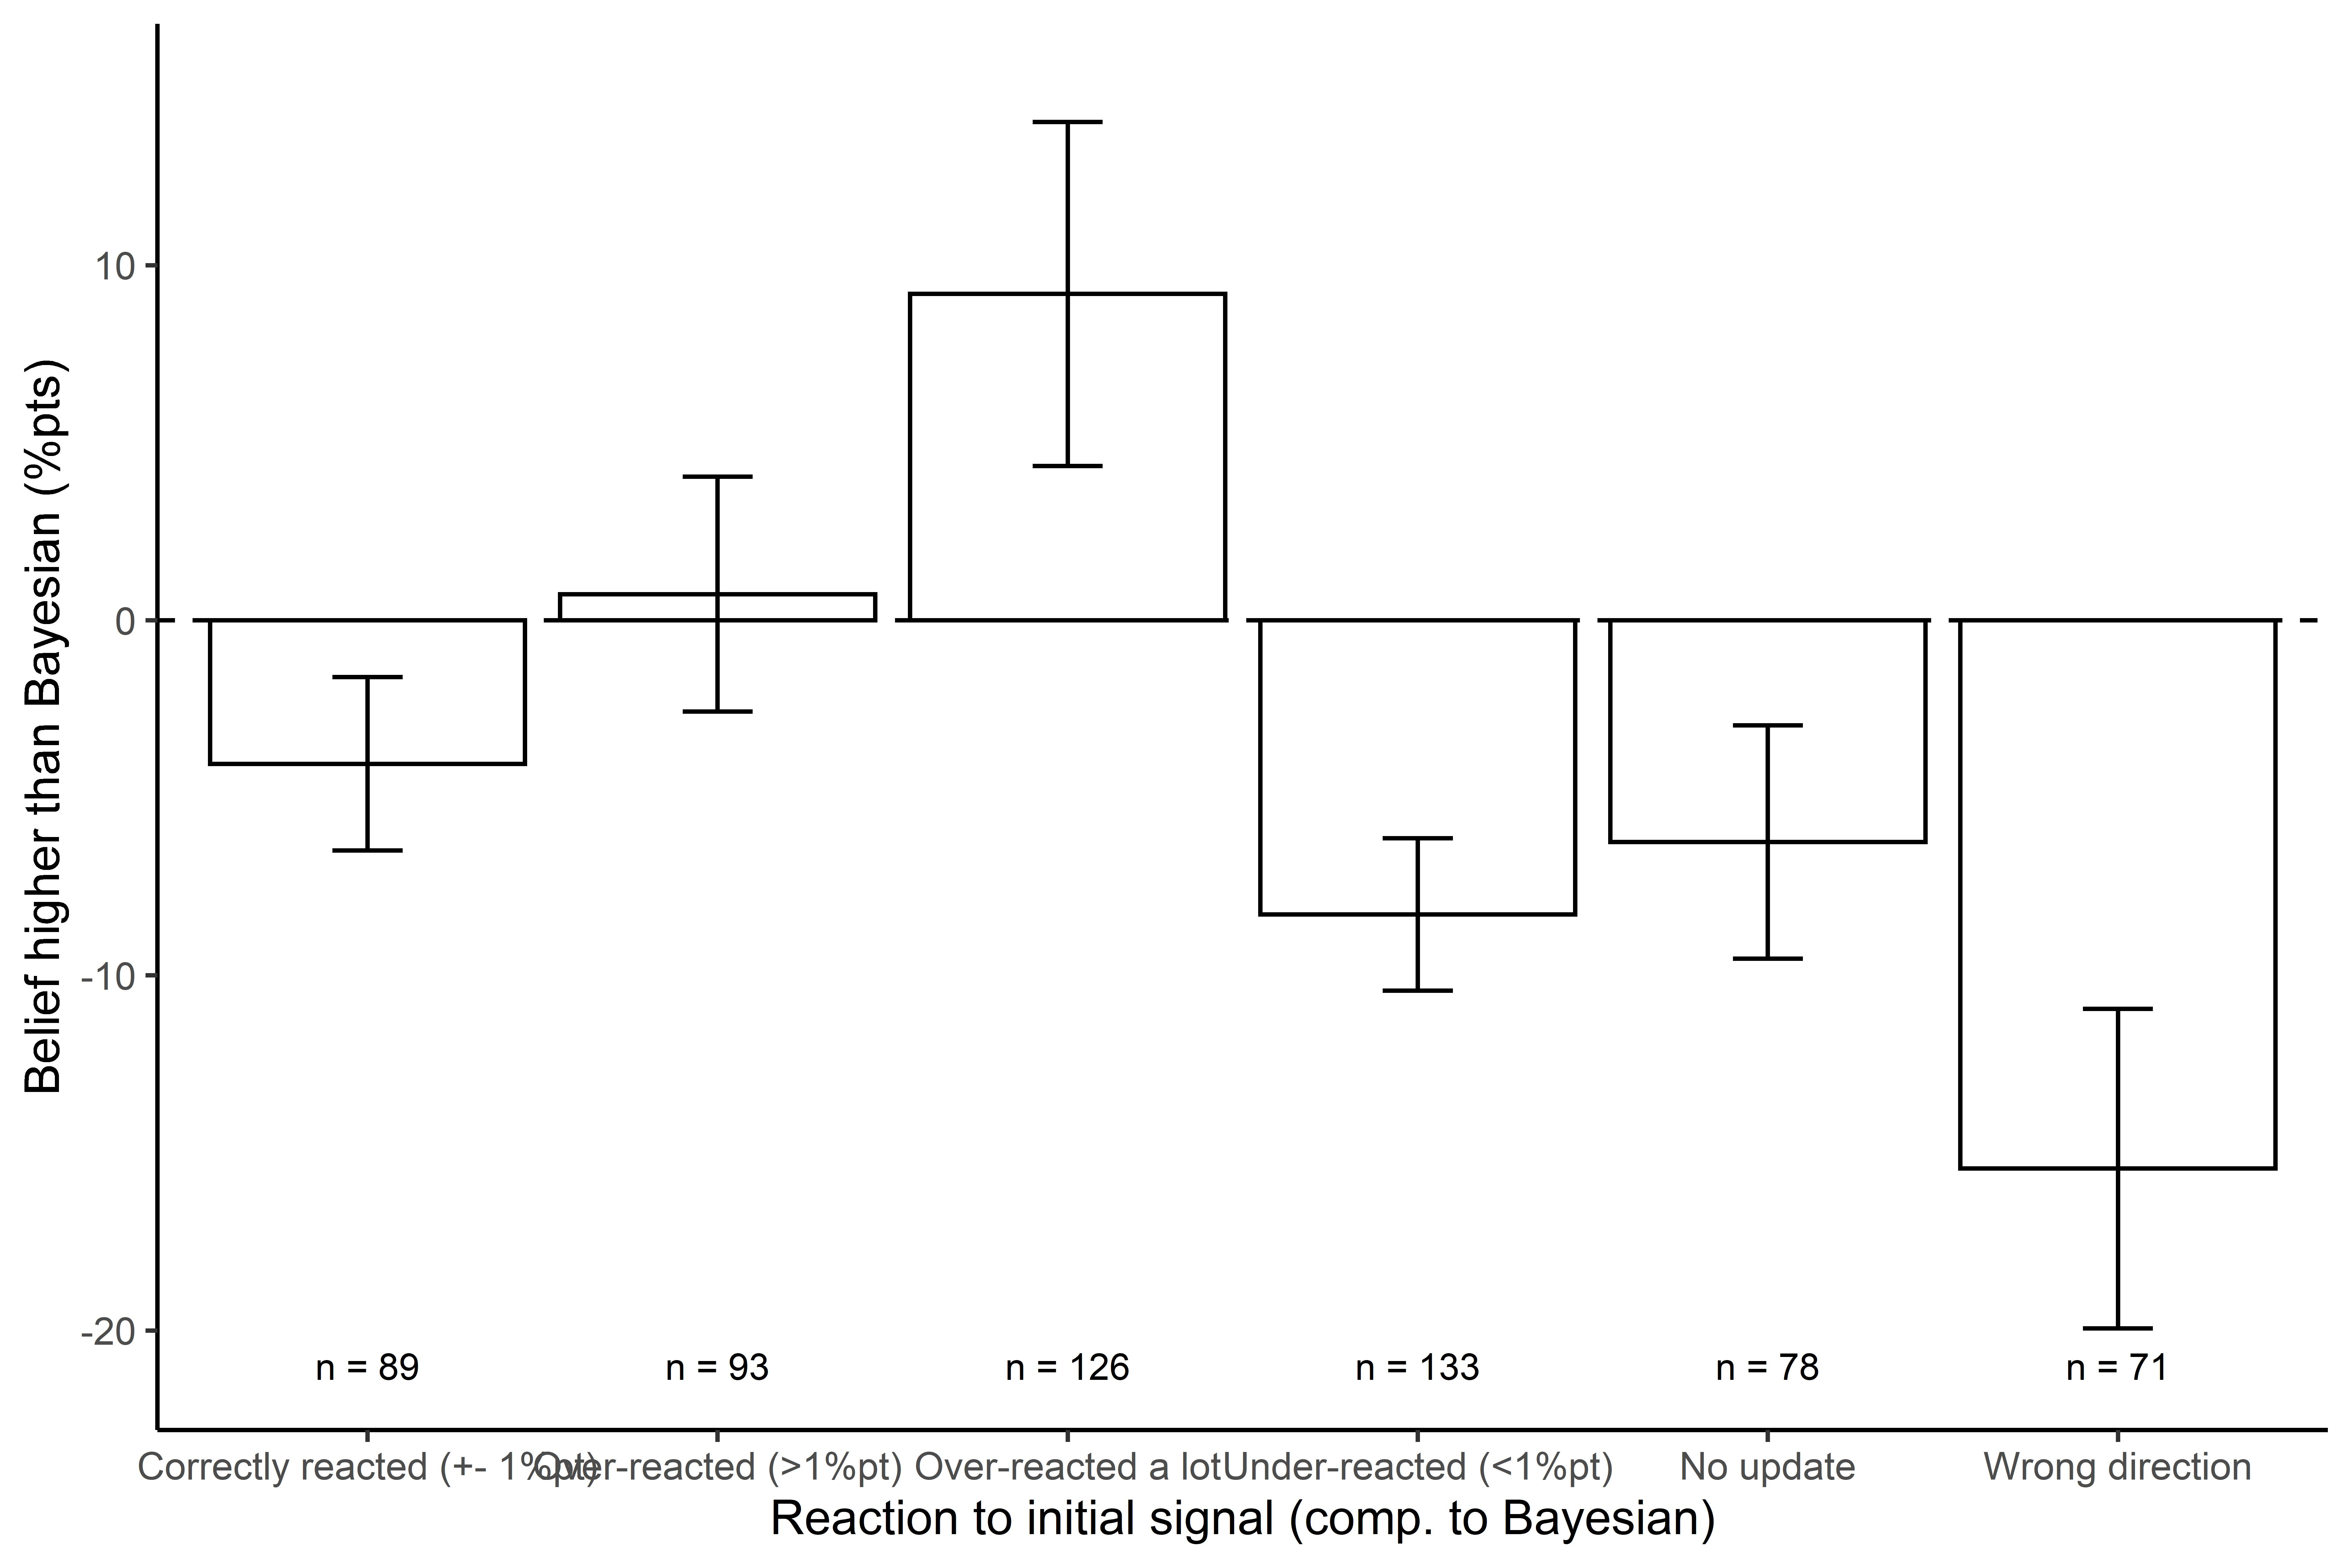
\includegraphics[width=12cm]{Fig/02_fig_confirm_diff.jpg}
    \caption{Reaction to confirmations. Influence of initial update on beliefs after the confirmation. This graph includes groups of people that were omitted in a previous table.}
    \label{fig:confirm_diff_complete}
\end{figure}


\newpage
\subsection{Ex-ante Verifications of Information}

% Table uninformative vs retraction - history FEs

% Table created by stargazer v.5.2.2 by Marek Hlavac, Harvard University. E-mail: hlavac at fas.harvard.edu
% Date and time: Mon, Jan 16, 2023 - 2:03:48 PM
\begin{table}[!htbp] \centering \footnotesize
  \caption{Uninformative Signals vs Retractions} 
  \label{tab:uninformative_vs_retractions} 
\begin{tabular}{@{\extracolsep{5pt}}lc} 
\\[-1.8ex]\hline 
\hline \\[-1.8ex] 
 & \multicolumn{1}{c}{\textit{Dependent variable:}} \\ 
\cline{2-2} 
\\[-1.8ex] & Reported Belief \\ 
 & All histories \\ 
\hline \\[-1.8ex] 
 Uninformative Signal: R & 0.044$^{*}$ \\ 
  & (0.023) \\ 
  Uninformative Signal: B & 0.029 \\ 
  & (0.024) \\ 
  Uninformative Signals: RR & $-$0.035 \\ 
  & (0.053) \\ 
  Uninformative Signals: BB & $-$0.055 \\ 
  & (0.047) \\ 
  Uninformative Signals: RB & 0.047 \\ 
  & (0.046) \\ 
  Uninformative Signals: BR & 0.222$^{***}$ \\ 
  & (0.067) \\ 
  Uninformative Signals: RRR & 0.017 \\ 
  & (0.082) \\ 
  Uninformative Signals: BBB & $-$0.032 \\ 
  & (0.097) \\ 
  Uninformative Signals: RRB & $-$0.341$^{*}$ \\ 
  & (0.182) \\ 
  Uninformative Signals: BBR & 0.082 \\ 
  & (0.105) \\ 
  Uninformative Signals: RBB & $-$0.320$^{*}$ \\ 
  & (0.182) \\ 
  Uninformative Signals: BRR & 0.409$^{**}$ \\ 
  & (0.182) \\ 
  Uninformative Signals: RBR & $-$0.070 \\ 
  & (0.108) \\ 
  Uninformative Signals: BRB & 0.001 \\ 
  & (0.111) \\ 
 \hline \\[-1.8ex] 
Aggregate History FEs? & Yes \\ 
Observations & 8,397 \\ 
Adjusted R$^{2}$ & 0.527 \\ 
\hline 
\hline \\[-1.8ex] 
\textit{Note:}  & \multicolumn{1}{r}{$^{*}$p$<$0.1; $^{**}$p$<$0.05; $^{***}$p$<$0.01} \\ 
\end{tabular} 
\end{table} 


% Table informative vs confirmation - history FEs

% Table created by stargazer v.5.2.2 by Marek Hlavac, Harvard University. E-mail: hlavac at fas.harvard.edu
% Date and time: Tue, Jan 17, 2023 - 11:31:46 AM
\begin{table}[!htbp] \centering \footnotesize
  \caption{Informative Signals vs Confirmations} 
  \label{tab:confirm_vs_informative} 
\begin{tabular}{@{\extracolsep{5pt}}lcc} 
\\[-1.8ex]\hline 
\hline \\[-1.8ex] 
 & \multicolumn{2}{c}{\textit{Dependent variable:}} \\ 
\cline{2-3} 
\\[-1.8ex] & \multicolumn{2}{c}{Reported Belief} \\ 
 & All histories & Excl. histories \\ 
 &  & with uninf. signals \\ 
\\[-1.8ex] & (1) & (2)\\ 
\hline \\[-1.8ex] 
 Informative Signal: R & 0.044 & 0.076$^{*}$ \\ 
  & (0.028) & (0.044) \\ 
  Informative Signal: B & 0.016 & 0.003 \\ 
  & (0.027) & (0.036) \\ 
  Informative Signals: RR & 0.103 & 0.033 \\ 
  & (0.070) & (0.205) \\ 
  Informative Signals: BB & 0.309$^{***}$ & $-$0.035 \\ 
  & (0.100) & (0.154) \\ 
  Informative Signals: RB & 0.025 & $-$0.058 \\ 
  & (0.075) & (0.105) \\ 
  Informative Signals: BR & $-$0.032 & $-$0.059 \\ 
  & (0.071) & (0.111) \\ 
  Informative Signals: RRR & 0.409$^{**}$ & 0.409$^{**}$ \\ 
  & (0.182) & (0.178) \\ 
  Informative Signals: BBB & $-$0.341$^{*}$ & $-$0.341$^{*}$ \\ 
  & (0.182) & (0.178) \\ 
  Informative Signals: RRB & 0.659$^{***}$ & 0.659$^{***}$ \\ 
  & (0.182) & (0.178) \\ 
  Informative Signals: BBR & 0.005 & 0.005 \\ 
  & (0.182) & (0.178) \\ 
  Informative Signals: RBB & 0.409$^{**}$ & 0.409$^{**}$ \\ 
  & (0.182) & (0.178) \\ 
  Informative Signals: BRR & 0.087 & 0.087 \\ 
  & (0.129) & (0.126) \\ 
  Informative Signals: RBR & $-$0.341$^{*}$ & $-$0.341$^{*}$ \\ 
  & (0.182) & (0.178) \\ 
 \hline \\[-1.8ex] 
Aggregate History FEs? & Yes & Yes \\ 
Observations & 8,397 & 7,319 \\ 
Adjusted R$^{2}$ & 0.527 & 0.536 \\ 
\hline 
\hline \\[-1.8ex] 
\textit{Note:}  & \multicolumn{2}{r}{$^{*}$p$<$0.1; $^{**}$p$<$0.05; $^{***}$p$<$0.01} \\ 
\end{tabular} 
\end{table} 



\newpage
\subsection{Impact of Previous Information Checks}

% Table LLR 

% Table created by stargazer v.5.2.2 by Marek Hlavac, Harvard University. E-mail: hlavac at fas.harvard.edu
% Date and time: Wed, Jan 11, 2023 - 4:00:35 PM
\begin{table}[!htbp] \centering \small
  \caption{Updating with Regular Signals} 
  \label{tab:regular_verifications_llr} 
\begin{tabular}{@{\extracolsep{5pt}}lcccc} 
\\[-1.8ex]\hline 
\hline \\[-1.8ex] 
 & \multicolumn{4}{c}{\textit{Dependent variable:}} \\ 
\cline{2-5} 
\\[-1.8ex] & \multicolumn{4}{c}{Observed Log-Posterior-Ratio} \\ 
\\[-1.8ex] & (1) & (2) & (3) & (4)\\ 
\hline \\[-1.8ex] 
 Constant & $-$0.042$^{*}$ & $-$0.041$^{*}$ & $-$0.040$^{*}$ & $-$0.039$^{*}$ \\ 
  & (0.022) & (0.022) & (0.022) & (0.022) \\ 
  Signal & 1.359$^{***}$ & 1.357$^{***}$ & 1.345$^{***}$ & 1.342$^{***}$ \\ 
  & (0.132) & (0.132) & (0.132) & (0.132) \\ 
  Prior & 0.485$^{***}$ & 0.486$^{***}$ & 0.477$^{***}$ & 0.478$^{***}$ \\ 
  & (0.036) & (0.036) & (0.036) & (0.036) \\ 
  Signal * Round & 0.078$^{**}$ & 0.080$^{**}$ & 0.084$^{**}$ & 0.086$^{**}$ \\ 
  & (0.038) & (0.038) & (0.038) & (0.038) \\ 
  Prior * Round & 0.031$^{***}$ & 0.031$^{***}$ & 0.030$^{***}$ & 0.030$^{***}$ \\ 
  & (0.004) & (0.004) & (0.004) & (0.004) \\ 
  Signal * \# Previously Checked Signals & $-$0.227$^{**}$ &  &  &  \\ 
  & (0.110) &  &  &  \\ 
  Signal * \# Previous Retractions &  & $-$0.178 &  &  \\ 
  &  & (0.117) &  &  \\ 
  Signal * \# Previous Confirmations &  & $-$0.321$^{**}$ &  &  \\ 
  &  & (0.132) &  &  \\ 
  Signal * \# Previous Same Checks &  &  & $-$0.066 &  \\ 
  &  &  & (0.119) &  \\ 
  Signal * \# Previous Other Checks &  &  & $-$0.430$^{***}$ &  \\ 
  &  &  & (0.123) &  \\ 
  Signal * \# Previous Same Retractions &  &  &  & $-$0.004 \\ 
  &  &  &  & (0.128) \\ 
  Signal * \# Previous Same Confirmations &  &  &  & $-$0.193 \\ 
  &  &  &  & (0.158) \\ 
  Signal * \# Previous Other Retractions &  &  &  & $-$0.400$^{***}$ \\ 
  &  &  &  & (0.135) \\ 
  Signal * \# Previous Other Confirmations &  &  &  & $-$0.482$^{***}$ \\ 
  &  &  &  & (0.162) \\ 
 \hline \\[-1.8ex] 
Observations & 4,860 & 4,860 & 4,860 & 4,860 \\ 
Akaike Inf. Crit. & 17,798.880 & 17,801.780 & 17,789.920 & 17,795.910 \\ 
\hline 
\hline \\[-1.8ex] 
\textit{Note:}  & \multicolumn{4}{r}{$^{*}$p$<$0.1; $^{**}$p$<$0.05; $^{***}$p$<$0.01} \\ 
\end{tabular} 
\end{table} 


% Table belief change

% Table created by stargazer v.5.2.2 by Marek Hlavac, Harvard University. E-mail: hlavac at fas.harvard.edu
% Date and time: Wed, Jan 11, 2023 - 4:00:36 PM
\begin{table}[!htbp] \centering \small
  \caption{Updating with Regular Signals} 
  \label{tab:regular_verifications_belief_change} 
\begin{tabular}{@{\extracolsep{5pt}}lcccc} 
\\[-1.8ex]\hline 
\hline \\[-1.8ex] 
 & \multicolumn{4}{c}{\textit{Dependent variable:}} \\ 
\cline{2-5} 
\\[-1.8ex] & \multicolumn{4}{c}{Belief change: $(b_t-b_{t-1})*I(s_t)$} \\ 
\\[-1.8ex] & (1) & (2) & (3) & (4)\\ 
\hline \\[-1.8ex] 
 Constant & 0.125$^{***}$ & 0.125$^{***}$ & 0.126$^{***}$ & 0.125$^{***}$ \\ 
  & (0.007) & (0.007) & (0.007) & (0.007) \\ 
  Round & $-$0.005$^{***}$ & $-$0.005$^{***}$ & $-$0.005$^{***}$ & $-$0.005$^{***}$ \\ 
  & (0.002) & (0.002) & (0.002) & (0.002) \\ 
  \# Previously Verified Signals & 0.004 &  &  &  \\ 
  & (0.005) &  &  &  \\ 
  \# Previous Retractions &  & 0.010$^{*}$ &  &  \\ 
  &  & (0.006) &  &  \\ 
  \# Previous Confirmations &  & $-$0.005 &  &  \\ 
  &  & (0.006) &  &  \\ 
  \# Previous Same Checks &  &  & 0.0003 &  \\ 
  &  &  & (0.006) &  \\ 
  \# Previous Other Checks &  &  & 0.009 &  \\ 
  &  &  & (0.006) &  \\ 
  \# Previous Same Retractions &  &  &  & 0.013$^{**}$ \\ 
  &  &  &  & (0.006) \\ 
  \# Previous Same Confirmations &  &  &  & $-$0.023$^{***}$ \\ 
  &  &  &  & (0.007) \\ 
  \# Previous Other Retractions &  &  &  & 0.006 \\ 
  &  &  &  & (0.006) \\ 
  \# Previous Other Confirmations &  &  &  & 0.015$^{**}$ \\ 
  &  &  &  & (0.007) \\ 
 \hline \\[-1.8ex] 
Observations & 4,860 & 4,860 & 4,860 & 4,860 \\ 
Adjusted R$^{2}$ & 0.006 & 0.008 & 0.007 & 0.013 \\ 
\hline 
\hline \\[-1.8ex] 
\textit{Note:}  & \multicolumn{4}{r}{$^{*}$p$<$0.1; $^{**}$p$<$0.05; $^{***}$p$<$0.01} \\ 
\end{tabular} 
\end{table} 



\newpage
\subsection{Additional}

\begin{figure}[!htb]
    \centering
    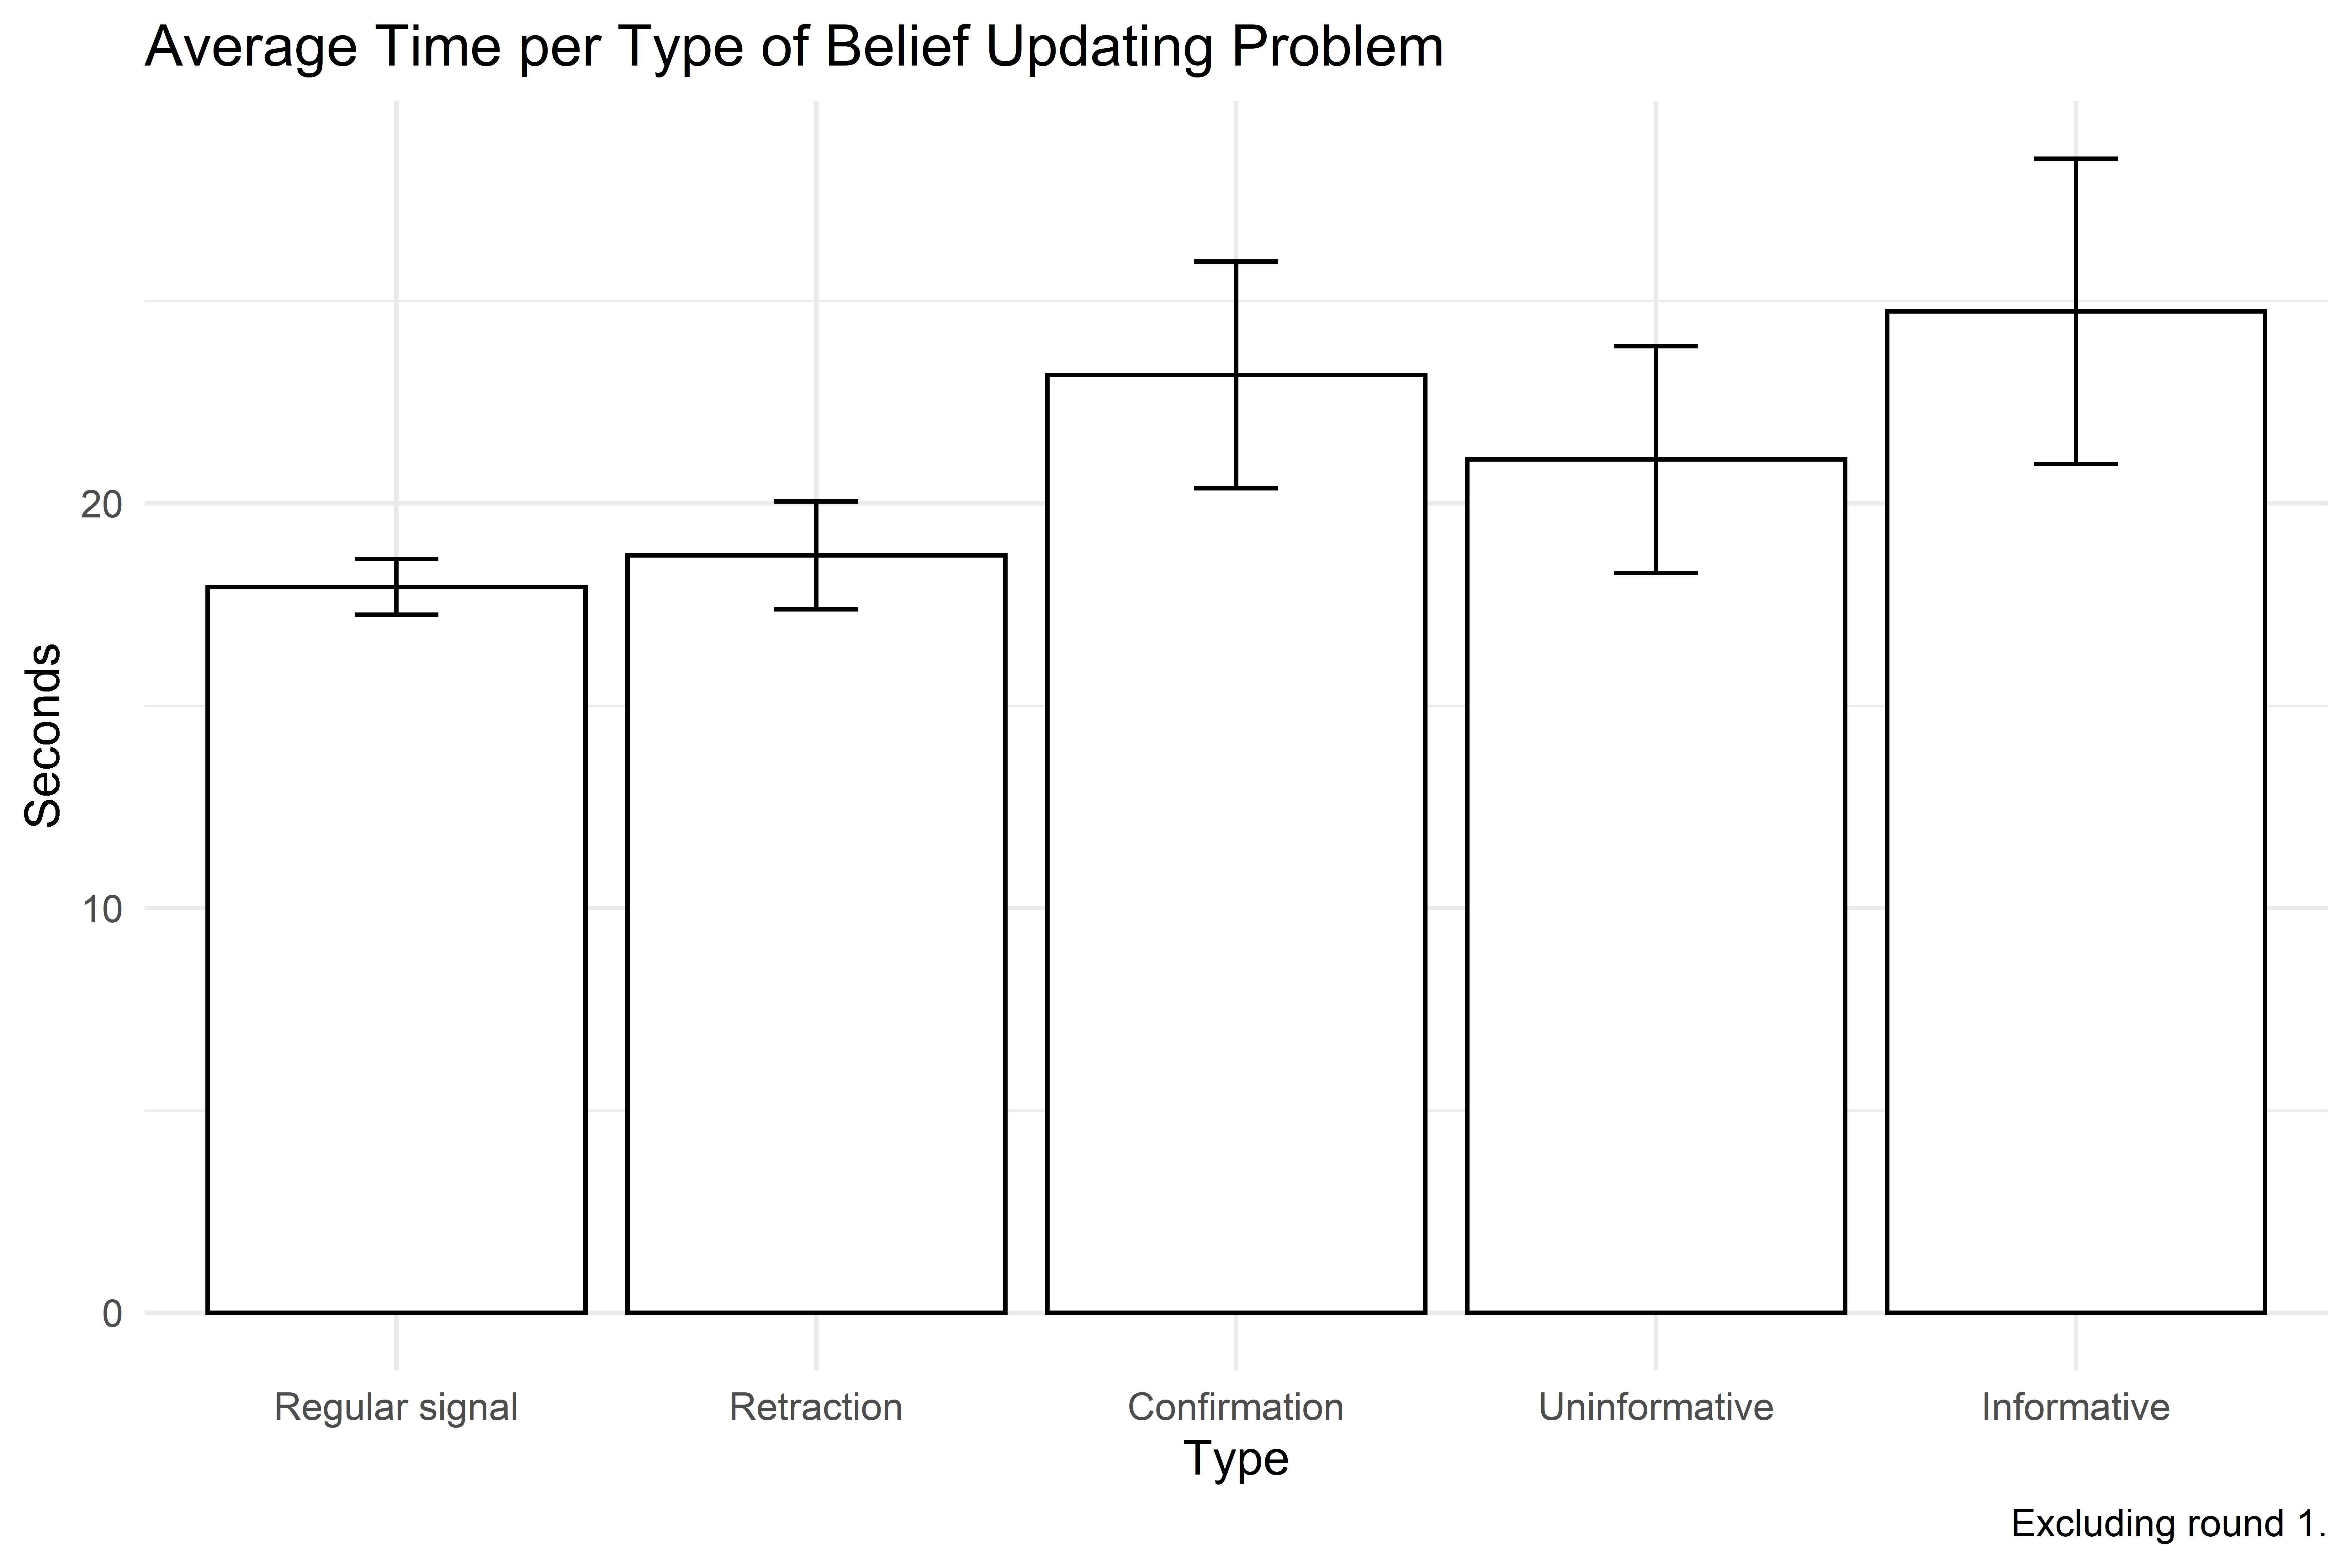
\includegraphics[width=12cm]{Fig/02_fig_time_belief_type.jpg}
    \caption{Time taken (in sec.) per type of belief updating problem. Round 1 was removed as subjects took far longer in this round. Confirmations seem to take people longer than retractions. No evidence that retractions take longer than regular updating.}
\end{figure}



\newpage
\section{Instructions and Screenshots}
\label{sec:instructions}

\subsection{Instructions - Ex-post Information Checks}
\noindent There are two urns, one red and one blue, each containing 4 balls as displayed below. All balls are labeled with a letter 'I', the meaning of which will be explained on the next page. One of the two urns will be randomly selected in the beginning. You do not know which urn will be selected. It will remain the same throughout this study. 

\vspace{1cm}
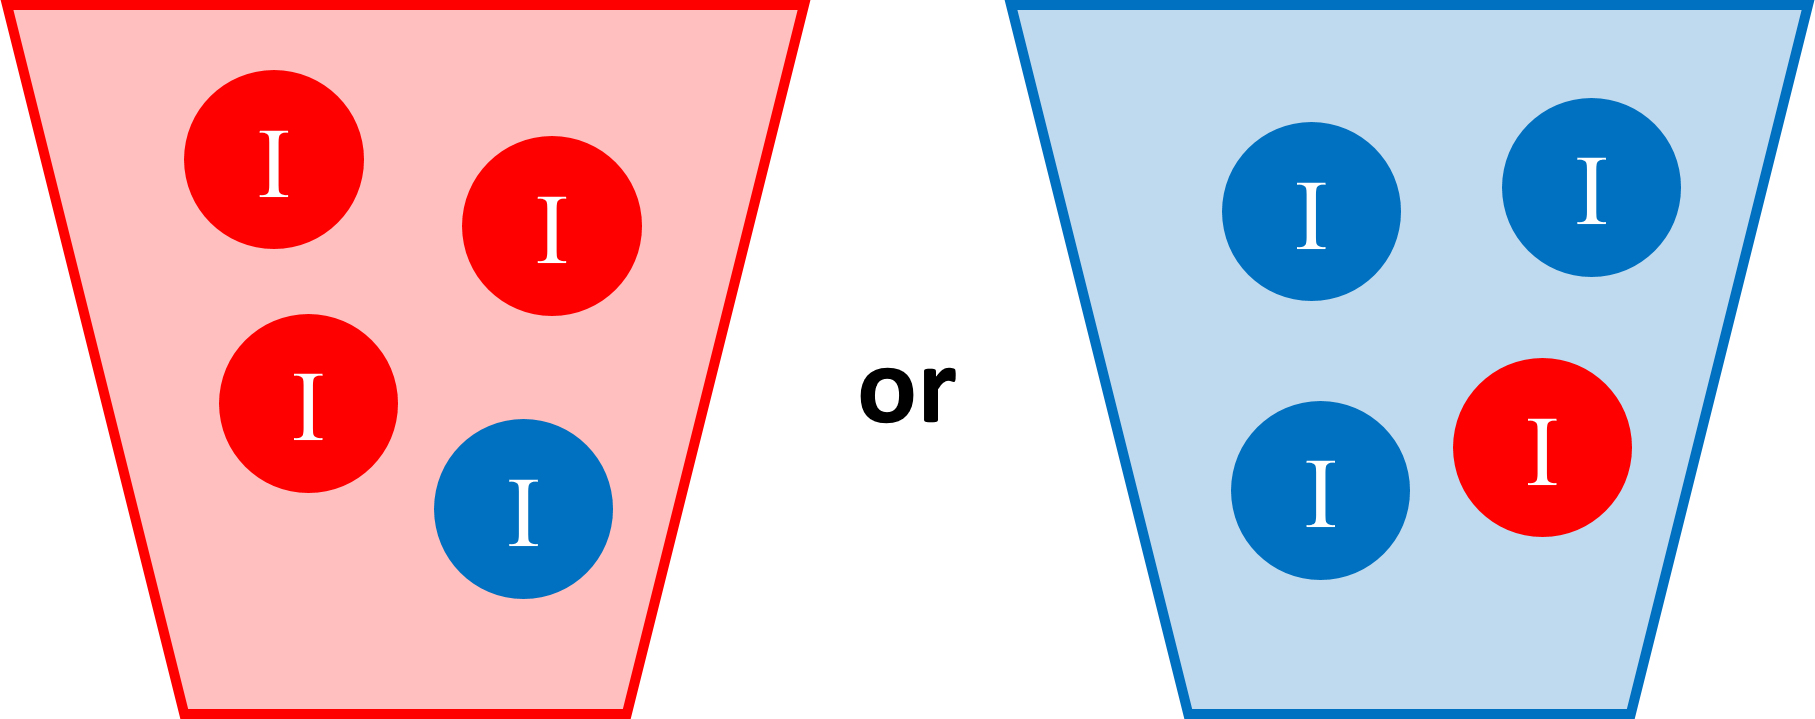
\includegraphics[width=8cm]{instructions/red_or_blue_urn.png}
\vspace{1cm}

\noindent Your \textbf{task will be to guess which urn you think was selected.} To do so you will receive hints about the selected urn. This will be described on the next page. 

-------------------------------------- [Page break] --------------------------------------

\noindent The selected urn contains 4 balls, 3 of the same color and 1 of the opposite color, as shown on the previous page. All balls from the selected urn are put into a black box. They are labeled with the letter 'I', which stands for 'informative'. If you knew the colour of all 4 balls, you would be able to identify the selected urn. For the moment you do not know the color of the selected urn and therefore the 4 informative balls are displayed in grey (although they have a color, either red or blue). 

\noindent The black box also contains 6 other balls that do not come from the urn. These 6 balls are labeled with the letter 'U', which stands for 'uninformative'. Knowing the color of the uninformative balls does not help to identify the selected urn. \textbf{The black box and the 10 balls inside it remain the same throughout the entire study. }

\vspace{1cm}
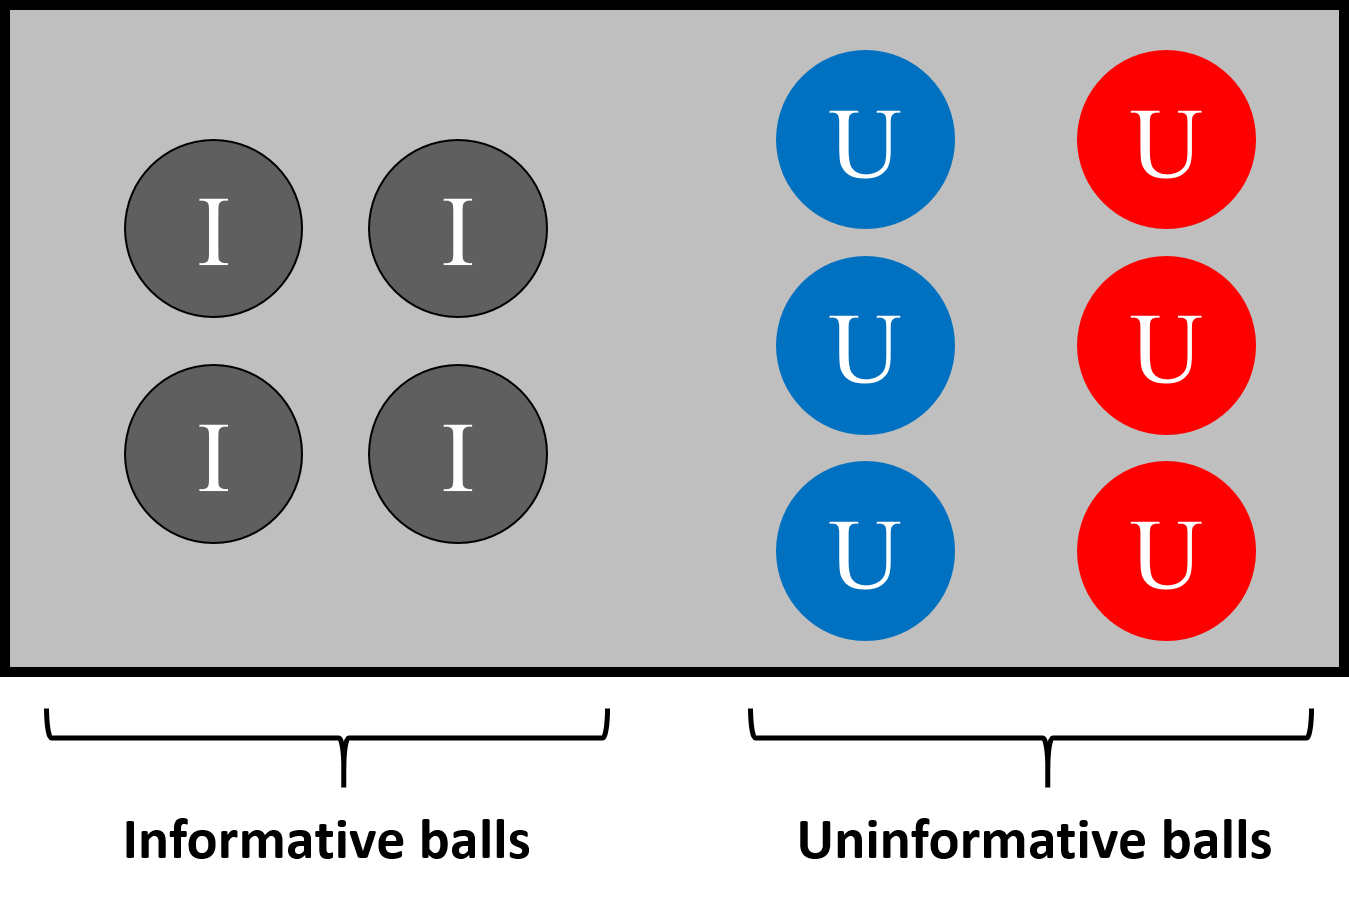
\includegraphics[width=8cm]{instructions/black_box.png}
\vspace{1cm}

This study has 12 rounds in total. In each round you get one of two possible hints: 
\begin{itemize}
    \item \textbf{A ball is drawn} from the black box. You are told the color of the ball. The ball is put back into the box together with the other 9 balls. You do not know if the balls is informative or uninformative. \textit{Example:} A red ball is drawn from the box. 
\includegraphics[width=0.5cm]{instructions/red_ball_q.png}
    \item No new ball is drawn, but you receive \textbf{information about the ball you saw previously}. You will be told if the ball you saw before was one of the 4 informative balls or one of the 6 uninformative balls. \textit{Example:} Previously you saw a red ball. The ball that was drawn last round was one of the 6 uninformative balls. 
\includegraphics[width=0.5cm]{instructions/red_ball_u.png} 
\end{itemize}

\noindent In every round you will be asked to make a guess about the urn that has been selected in the beginning. At the end of the study you will be told the color of this urn. You will receive a bonus which depends on the accuracy of your answer to one of the 12 guesses (you do not know which one). The procedure for calculating your bonus is described in detail below. You may skip these details. The important thing is that the procedure guarantees that you should expect to maximize your bonus by reporting what you truly think the chances are in each question. 

-------------------------------------- [Button: 'Details about the bonus'] --------------------------------------

\noindent\textbf{We apply the following procedure: 
}

\noindent First, we randomly pick one of the questions. For this question, we calculate the error you made. This is how many percentage points your report was away from 100\% (if the RED URN was selected) or from 0\% (if the BLUE URN was selected). Then, we plug in the error into the following formula: 

$$3-3 \cdot \text{error}^2$$

 \noindent This will be your bonus (in Euros). 

\noindent\textbf{EXAMPLE:} Suppose that you report 60\% chance that the RED URN was selected in Step 1. Then, your bonus is calculated as follows: 
\begin{itemize}
    \item If the urn was RED:
    \begin{itemize}
        \item your error is $(100\%-60\%) = 40\%$
        \item your bonus is $3-3\cdot (40\%)^2 = 2.52 \text{Euros}$
    \end{itemize}
    \item If the urn was BLUE:
    \begin{itemize}
        \item your error is $(60\%-0\%) = 60\%$
        \item your bonus is $3-3\cdot (60\%)^2 = 1.92 \text{Euros}$
    \end{itemize}
\end{itemize}

\noindent As we have already mentioned, you should expect to maximize your earnings by reporting what you actually think are the chances of a RED URN. 

\noindent \textbf{Example:} If you actually think that the chances are 60\% that the RED URN was selected, then:
\begin{itemize}
    \item By reporting 60\%, you will make on average 2.28 Euros.
    \item By reporting 10\%, you will make on average 1.53 Euros.
    \item By reporting 100\%, you will make on average 1.80 Euros.
\end{itemize}

\noindent As you see you maximize your earning by reporting exactly 60\%. The further away you report from what you actually think, the less money you should expect to make.




\subsection{Instructions - Ex-ante Information Verification}
\noindent There are two urns, one red and one blue, each containing 4 balls as displayed below. All balls are labeled with a letter 'I', the meaning of which will be explained on the next page. One of the two urns will be randomly selected in the beginning. You do not know which urn will be selected. It will remain the same throughout this study. 

\vspace{1cm}
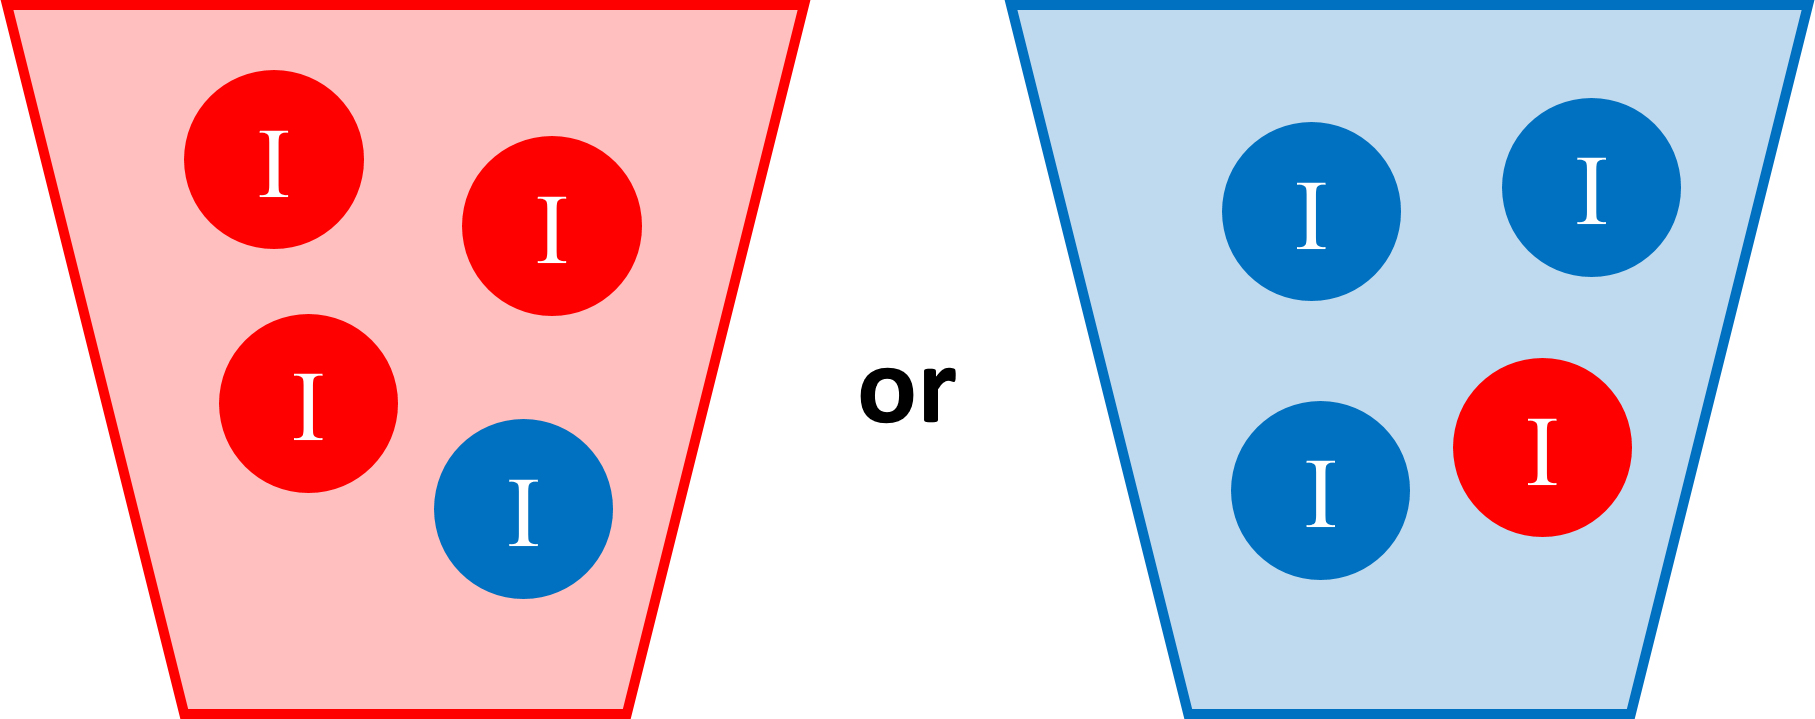
\includegraphics[width=8cm]{instructions/red_or_blue_urn.png}
\vspace{1cm}

\noindent Your \textbf{task will be to guess which urn you think was selected.} To do so you will receive hints about the selected urn. This will be described on the next page. 

-------------------------------------- [Page break] --------------------------------------

\noindent The selected urn contains 4 balls, 3 of the same color and 1 of the opposite color, as shown on the previous page. All balls from the selected urn are put into a black box. They are labeled with the letter 'I', which stands for 'informative'. If you knew the colour of all 4 balls, you would be able to identify the selected urn. For the moment you do not know the color of the selected urn and therefore the 4 informative balls are displayed in grey (although they have a color, either red or blue). 

\noindent The black box also contains 6 other balls that do not come from the urn. These 6 balls are labeled with the letter 'U', which stands for 'uninformative'. Knowing the color of the uninformative balls does not help to identify the selected urn. \textbf{The black box and the 10 balls inside it remain the same throughout the entire study. }

\vspace{1cm}
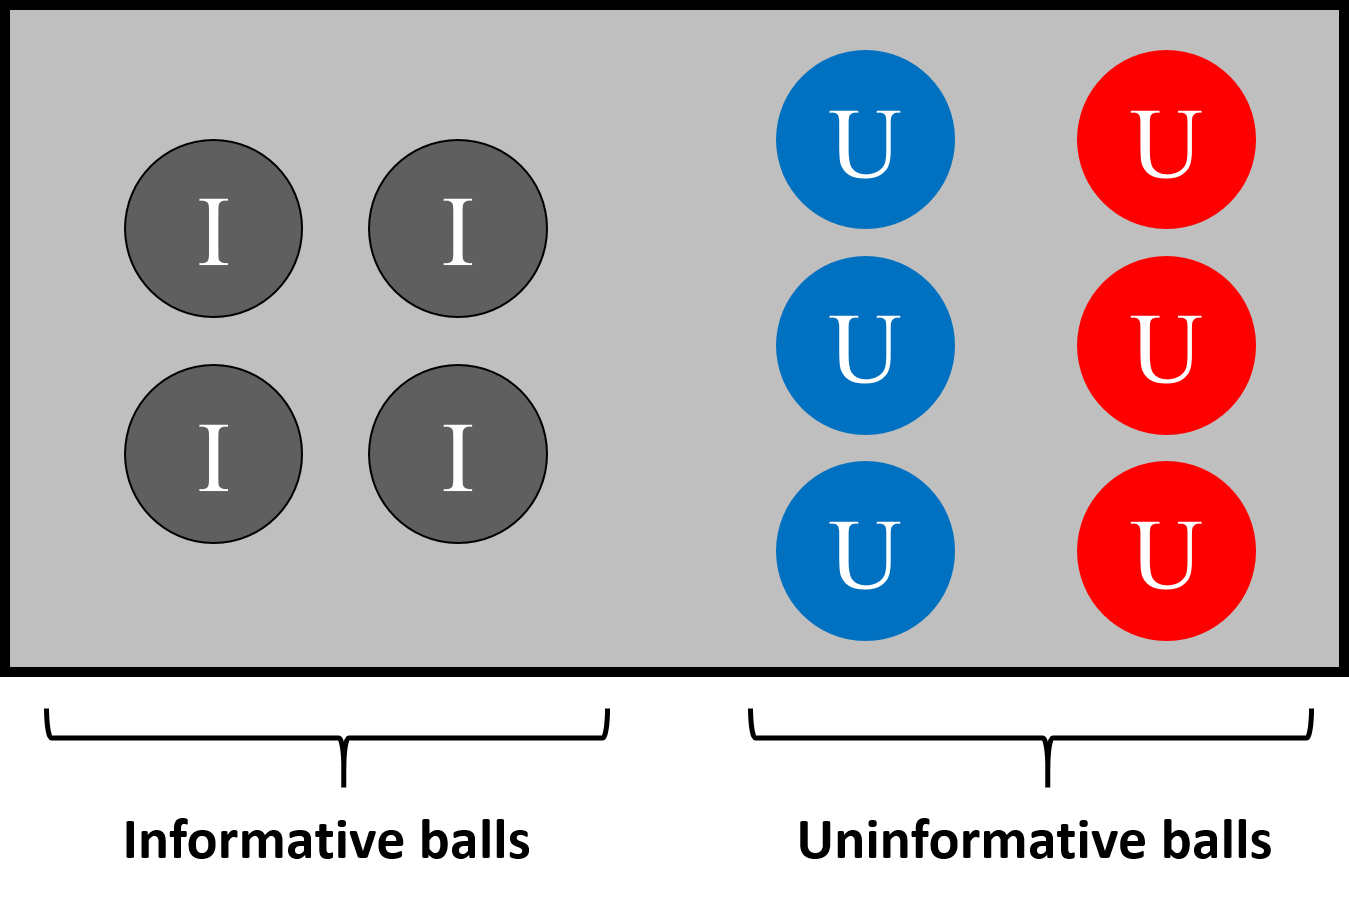
\includegraphics[width=8cm]{instructions/black_box.png}
\vspace{1cm}

This study has 9 rounds in total. In each round a ball is drawn from the black box and you get one of two possible hints: 
\begin{itemize}
    \item You are \textbf{told only the color} of the ball. The ball is put back into the box together with the other 9 balls. You do not know if the ball is informative or uninformative. \textit{Example:} A red ball was drawn from the box. 
\includegraphics[width=0.5cm]{instructions/red_ball_q.png}
    \item You are \textbf{told the color and the letter} on the ball. The ball is put back into the box together with the other 9 balls. You know if the ball is informative or entirely uninformative. \textit{Example:} A red ball was drawn from the box. It is one of the 4 informative balls: 
\includegraphics[width=0.5cm]{instructions/red_ball_u.png} 
\end{itemize}

\noindent In every round you will be asked to make a guess about the urn that has been selected in the beginning. At the end of the study you will be told the color of this urn. You will receive a bonus which depends on the accuracy of your answer to one of the 12 guesses (you do not know which one). The procedure for calculating your bonus is described in detail below. You may skip these details. The important thing is that the procedure guarantees that you should expect to maximize your bonus by reporting what you truly think the chances are in each question. 

-------------------------------------- [Button: 'Details about the bonus'] --------------------------------------

\noindent\textbf{We apply the following procedure: 
}

\noindent First, we randomly pick one of the questions. For this question, we calculate the error you made. This is how many percentage points your report was away from 100\% (if the RED URN was selected) or from 0\% (if the BLUE URN was selected). Then, we plug in the error into the following formula: 

$$3-3 \cdot \text{error}^2$$

 \noindent This will be your bonus (in Euros). 

\noindent\textbf{EXAMPLE:} Suppose that you report 60\% chance that the RED URN was selected in Step 1. Then, your bonus is calculated as follows: 
\begin{itemize}
    \item If the urn was RED:
    \begin{itemize}
        \item your error is $(100\%-60\%) = 40\%$
        \item your bonus is $3-3\cdot (40\%)^2 = 2.52 \text{Euros}$
    \end{itemize}
    \item If the urn was BLUE:
    \begin{itemize}
        \item your error is $(60\%-0\%) = 60\%$
        \item your bonus is $3-3\cdot (60\%)^2 = 1.92 \text{Euros}$
    \end{itemize}
\end{itemize}

\noindent As we have already mentioned, you should expect to maximize your earnings by reporting what you actually think are the chances of a RED URN. 

\noindent \textbf{Example:} If you actually think that the chances are 60\% that the RED URN was selected, then:
\begin{itemize}
    \item By reporting 60\%, you will make on average 2.28 Euros.
    \item By reporting 10\%, you will make on average 1.53 Euros.
    \item By reporting 100\%, you will make on average 1.80 Euros.
\end{itemize}

\noindent As you see you maximize your earning by reporting exactly 60\%. The further away you report from what you actually think, the less money you should expect to make.






\subsection{Example screen with ball draw}

We have three treatments to vary information display. One version is displayed below. In the other two we either do not display the table containing the history of previous signals or we do not display the sentence reminding people of their previously reported belief. All else stays the same. It should also be noted that currently no default belief is selected on the slider. Once the subject clicks on the slider an icon appears. Also, the belief is displayed below it in front of the percentage symbol.

% Example screen
\begin{figure}[!htb]
    \centering
    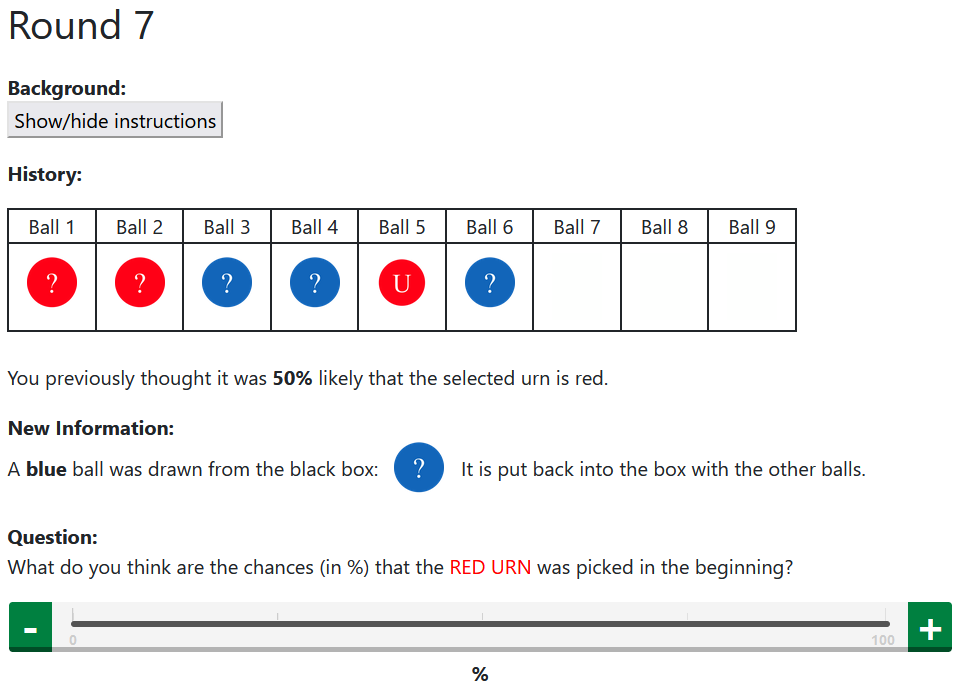
\includegraphics[width=15cm]{Fig/screen.png}
    \caption{Example Screen}
    \label{fig:example_screen}
\end{figure}



\end{document}
